\chapter{Search for heavy scalar or pseudoscalar bosons in \ttbartitle final states}
\label{ch:ah}

\section{Introduction}
\label{sec:ah:intro}

Additional spin-0 particles are predicted in many attractive extensions of the Standard Model, and can be searched for in \ttbar final states at the LHC if the new states are heavy (i.e. have a mass larger than $2\mt$), electrically neutral, and exhibit Yukawa-like couplings to fermions (see \cref{sec:theory:ah}). A generic model for such states with either pseudoscalar (A) or scalar (H) couplings to top quarks was given in \cref{eq:theory:lag_ah}.

In addition, \ttbar bound state effects are expected in the SM in several calculations, with a pseudoscalar component dominating at the LHC as discussed in \cref{sec:theory:etat}. Since the experimental invariant mass resolution for the \ttbar final state is rather coarse, additional BSM particles and bound state effects are expected to lead to similar experimental signatures, and it thus makes sense to search for them for using the same methods.

%and searches for such particles at the LHC have potential of discovering hints for new physics. Oftentimes, such models predict Yukawa-type couplings for the new particles to SM fermions, which scale with the fermion mass. It is thus natural to search for interactions of new spin-0 states with the heaviest fundamental particle in the SM: the top quark.

%In particular, if the mass of any such new state is larger than double the top quark mass, it can decay to a \ttbar final state. This decay channel will be dominant in many scenarios. If the new state is produced in gluon fusion, the resulting process will interfere with SM \ttbar production as discussed in \cref{sec:theory:ttbar}, leading to an interference pattern in the invariant \ttbar mass that can be probed experimentally.

%To do so, a generic model describing the new particles is defined, containing two new spin-0 states A and H which both couple solely to the top quark via a pseudoscalar (for A) and a scalar (for H) Yukawa interaction. The Lagrangian reads

%\begin{equation}
%\label{eq:ah:lagrangian}
%\begin{split}
%    \mathcal{L}_{\AH} =& \, \frac{1}{2} (\partial_\mu A ) (\partial^\mu A ) +\frac{\mA^2}{2} A^2  
%    + i  \gAtt \, \frac{\mt}{v} \bar t  \gamma_5 \, t  \, A \\
%    & + \frac{1}{2} (\partial_\mu H ) (\partial^\mu H ) +\frac{\mH^2}{2} H^2  
%    -  \gHtt \, \frac{\mt}{v} \bar t \, t  \, H \,
%\end{split}
%\end{equation}

%Here, \mA and \mH are the masses of the new particles, \gAtt and \gHtt are the coupling modifiers for the top quark Yukawa couplings, \mt is the top quark mass, and $v$ is the vacuum expectation value of the SM Higgs boson. 

%This model assumes that the two states A and H do not mix, which is equivalent to the assumption that there is no \CP violation [??]. Apart from this assumption, it is fully generic and can be mapped onto any of the models discussed in \cref{sec:theory:ah}, provided that only couplings to the top quark are considered. This makes it ideal for an experimental search, as results presented using this model can be easily reinterpreted in various models of interest.

%In addition to the masses and coupling modifiers, the decay widths \wA and \wH of the two particles are also considered as free parameters, yielding six free parameters total. This is because, due to interactions with other SM particles besides the top quark, or with additional BSM particles, concrete models (e.g. the 2HDM) will predict different decay widths then the natural width expected in the simplified model. In particular, if either or both of the particles is to be considered a dark matter mediator, it will have a significant branching ratio to dark matter particles, increasing its absolute width.

This chapter presents such a search for new spin-0 states with either scalar or pseudoscalar interactions with the top quark, using the full Run~2 data set with an integrated luminosity of \SI{138}{\fbinv} at the CMS experiment. It follows up on a similar search done using only \SI{35.9}{\fbinv} of data taken in 2016~\cite{CMS:HIG-17-027}. Similar searches have also been published by ATLAS, one with \SI{20.3}{\fbinv} of data taken at $\sqrt{s}=\SI{8}{\TeV}$~\cite{ATLAS:2017snw} and one with \SI{140}{\fbinv} of data taken at $\sqrt{s}=\SI{13}{\TeV}$~\cite{ATLAS:2024vxm}.

The work done as part of this thesis focused on the dilepton decay channel of \ttbar, which is thus described in detail in~\cref{sec:ah:setup,sec:ah:ttbarweights,sec:ah:mereweighting,sec:ah:systs,sec:ah:prefit}. A significant excess of events is observed at invariant masses close to the \ttbar threshold, which is interpreted either as a pseudoscalar \ttbar bound state (\cref{sec:ah:etat,sec:ah:parityscan,sec:ah:checks}) or as an additional scalar or pseudoscalar boson (\cref{sec:ah:bestfitah}). For the latter interpretation, exclusion limits for a large mass range are also presented in \cref{sec:ah:limits}. Following this, the dilepton channel is combined with a similar analysis of the \ljets decay channel, which is discussed in \cref{sec:ah:combination}, and exclusion regions are provided for the presence of either one or two additional bosons. Finally, the results of this work are briefly compared in \cref{sec:ah:comparison} to those of \citere{ATLAS:2024vxm}, in which no excess was observed, as well as to other \ttbar measurements, and a summary and outlook are given in \cref{sec:ah:summary}.

The results presented here were first made public as a Physics Analysis Summary~\cite{CMS:HIG-22-013-PAS}, and later submitted to \textit{Reports on Progress in Physics} in an updated form focusing solely on the interpretation of a \ttbar bound state~\cite{CMS:TOP-24-007}. A further submission focusing on the interpretation in terms of additional bosons is in preparation. They are the continuation of a previous PhD thesis~\cite{Rubenach:PhD}, in which the analysis strategy of the dilepton channels as well as the procedure of obtaining exclusion limits for additional bosons was designed. Following up on this, the contribution of the work at hand consists of the implementation of matrix element reweighting for the signal simulation (\cref{sec:ah:mereweighting}), the simulation of the \ttbar bound state signal (\cref{sec:theory:etat}), the interpretation of the observed excess in terms of \ttbar bound states or additional bosons including all corresponding cross-checks (\cref{sec:ah:excess}), the comparison to other results (\cref{sec:ah:comparison}), and the preparation of the results for publication in Refs.~\cite{CMS:HIG-22-013-PAS} and \cite{CMS:TOP-24-007}.

\section{Analysis setup}
\label{sec:ah:setup}

This section describes the analysis strategy in the dilepton channels, consisting of the considered data sets, object definitions, event selection criteria, corrections and reconstruction algorithms.

\subsection{Data sets}
\label{sec:ah:datasets}

\paragraph{Experimental data} 
The analysis is performed using the full CMS Run~2 ultra-legacy (UL) data set, which is the final, re-reconstructed and recalibrated data set recommended by CMS for physics analyses. It is split into the three data taking years of Run~2: 2016, 2017 and 2018, where 2016 is further split into two parts, denoted ``2016pre'' and ``2016post", because of a modification of the APV readout chip settings that affects the efficiency of the track hit reconstruction during the 2016 data-taking period~\cite{CMS-DP-2020-045}.

A similar combination of dilepton and single-lepton triggers as in \cref{sec:ttxs:datasets} is used for all years, with the \pt thresholds varying slightly between data taking eras, as shown in \cref{tab:ah:triggers}. 

\begin{table}
\centering
\begin{tabular}{c|c|c}
    Trigger & Year & Lepton \pt requirement \\
    \hline
    \hline
    \multirowcell{3}{single-e} & 2016 & e~($\pt > \SI{27}{\GeV}$) \\
    & 2017 & e~($\pt > \SI{35}{\GeV}$) \\
    & 2018 & e~($\pt > \SI{32}{\GeV}$) \\
    \hline
    \multirowcell{3}{single-\textmu} & 2016 & \textmu~($\pt > \SI{24}{\GeV}$) \\
    & 2017 & \textmu~($\pt > \SI{27}{\GeV}$) \\
    & 2018 & \textmu~($\pt > \SI{24}{\GeV}$) \\
    \hline
    \multirowcell{2}{\emu} & \multirowcell{2}{all} & e~($\pt > \SI{12}{\GeV}$) and \textmu~($\pt > \SI{23}{\GeV}$) or \\
    & & e~($\pt > \SI{23}{\GeV}$) and \textmu~($\pt > \SI{8}{\GeV}$) \\
    \hline
    \ee & all & $\text{e}_1$~($\pt > \SI{23}{\GeV}$) and $\text{e}_2$~($\pt > \SI{12}{\GeV}$) \\
    \hline
    \mumu & all & $\text{\textmu}_1$~($\pt > \SI{17}{\GeV}$) and $\text{\textmu}_2$~($\pt > \SI{8}{\GeV}$)
\end{tabular}
\caption{\textbf{Trigger \pt thresholds.} Overview of the used triggers in the three data taking years, as well as their lepton \pt thresholds.}
\label{tab:ah:triggers}
\end{table}

\paragraph{Background simulation}
Since the final state of the signals considered in this analysis are the same as in the SM \ttbar background, it is clear that a large irreducible background is expected. As a result, it is essential that the SM Monte Carlo simulation is as both theoretically precise and has sufficient statistics, and that any remaining imprecisions are covered by the systematic uncertainty model.

The SM \ttbar background is again simulated at NLO in QCD with the \texttt{hvq} process from the  MC generator package \powhegvtwo and interfaced to \textsc{Pythia 8} for showering. Similar settings as in \cref{sec:ttxs:datasets} have been used. To achieve the necessary precision, the NLO simulation is reweighted to higher orders in both QCD and electroweak (EW) processes, which is described in \cref{sec:ah:ttbarweights}.

In addition, several minor backgrounds are included, a summary of which can be found in \cref{tab:ah:simulation}. Of note here is the Z+jets background, which is simulated at NNLO in QCD using the Mingle method in \powhegvtwo. It was found here that the higher-order corrections are relevant to the analysis especially for low values of the invariant dilepton mass \mll. Most processes are normalized to cross sections predicted at higher orders of QCD where available, which can be found in \cref{tab:ah:crosssections}.

\begin{table}
    \centering\renewcommand\arraystretch{1.2}
    \begin{tabular}{c|c|c}
     Process & QCD order & ME Generator \\
     \hline
     \hline
     \ttbar & NLO & \powhegvtwo (\texttt{hvq}) \\
     tW & NLO & \powhegvtwo (\texttt{ST\_wtch}) \\
     \Zgamma+jets & NNLO & \powhegvtwo (\texttt{Zj} MiNNLO) \\
     $t$-channel single top & NLO & \powhegvtwo (\texttt{ST\_tch}) + \textsc{MadSpin} \\
     $s$-channel single top & NLO & \amcatnlo \\
     $\ttbar \mathrm{W}$ & NLO & \amcatnlo \\
     $\ttbar \mathrm{Z}$ & NLO & \amcatnlo \\
     WW, WZ \& ZZ & LO & \pythia 8.2 \\
     \hline
     \AH signal & LO & \amcatnlo \\
     \etat signal & LO & \amcatnlo
\end{tabular}
\caption{\textbf{Simulated background and signal samples.} An overview of the different background and signal processes considered, as well as the theoretical order in QCD and the ME generator used to simulate them. For all samples, \textsc{Pythia 8.2} is used for showering and hadronization.}
\label{tab:ah:simulation}
\end{table}

\begin{table}
    \centering\renewcommand\arraystretch{1.2}
    \begin{tabular}{c|c|c|c}
         Process & Cross section (pb) & Order & Program / reference \\
         \hline
         \hline
         \ttbar & 833.9 & NNLO+NNLL & Top++~\cite{Czakon:2011xx} \\
         tW & 71.7 & NNLO (approx.) & \cite{Kidonakis:2021vob} \\
         $t$-channel single top & 217.0 & NLO & Hathor~\cite{Aliev:2010zk,Kant:2014oha} \\
         $s$-channel single top & 10.3 & NLO & Hathor~\cite{Aliev:2010zk,Kant:2014oha} \\
         $\ttbar \mathrm{W}$ & 0.64 & NLO & \amcatnlo \\
         $\ttbar \mathrm{Z}$ & 0.75 & NLO & \amcatnlo \\
         $\Zgamma\mathrm{+jets} \rightarrow \ell\ell$, & \multirowcell{2}{$24.7 \times 10^3$} & \multirowcell{2}{NNLO} & \multirowcell{2}{FEWZ~\cite{Melnikov:2006kv,Li:2012wna}}  \\
         $\mll > \SI{10}{\GeV}$ & & & \\
         WW & 118.7 & NNLO & \cite{Gehrmann:2014fva} \\
         WZ & 471.3 & NLO & MCFM~\cite{Campbell:2010ff} \\
         ZZ & 165.2 & NLO & MCFM~\cite{Campbell:2010ff}
    \end{tabular}
    \caption{\textbf{Cross sections for background processes.} The cross sections used for the normalization of background processes relevant for this search, as well as the orders in QCD at which they were computed.}
    \label{tab:ah:crosssections}
\end{table}

\paragraph{Signal simulation}

The signal for the general \AH model described in \cref{sec:ah:intro} is generated at LO in QCD using \madgraph with a custom Universal FeynRules Output (UFO) model. The $\mathrm{pp} \to \AH \to \ttbar$ resonance and the \AH-SM interference are simulated separately, and both are again showered with \textsc{Pythia 8}. In order to cover the phase space of the \AH model, the signals are generated for all combinations of the following values of the \AH masses and widths:

\begin{equation}
\begin{split}
    m_{\AH} &\in \{ 365, 400, 500, 600, 800, 1000 \} \, \si{\GeV} \\
    \Gamma_{\AH} / m_{\AH} &\in \{ 2.5, (5), 10, 25 \} \, \%
\end{split}
\end{equation}

Samples with a width of $5\%$ were generated only for a mass of \SI{400}{\GeV}, which leads to 38 signal points total. In addition, samples for the pseudoscalar case only were generated with

\begin{equation}
    \mA \in \{ 450, 550, 700, 900 \} \, \si{GeV}, \quad \wA / \mA = 9 \, \%.
\end{equation}

All of these samples were combined and used reweighted at matrix element level to obtain also phase space points between these mass and width values, as described further in \cref{sec:ah:mereweighting}.

Furthermore, signal samples for possible \ttbar bound state effects are generated using the color-singlet \etat and \chit models as defined in \cref{sec:theory:etat}, using custom UFO models implemented in \madgraph and again showered with \pythia.

For all signal and background samples, the detector response is simulated with \textsc{Geant 4} and the full CMS simulation and reconstruction chain as described in \cref{sec:mc:detector} is performed.

\subsection{Object definition}
\label{sec:ah:objects}

\paragraph{Leptons} 

All electrons and muons are required to have $\pt > \SI{20}{\GeV}$ and $\abseta < 2.4$ to be considered for the analysis. Similar to \cref{sec:ttxs:objects}, electrons in the transition region between barrel and endcaps in the ECAL are removed, and additional ID criteria are applied for both types of leptons.

For electrons, the multivariate classifier (MVA)-based ID described in \citere{CMS:EGM-17-001} is used at a working point giving 90 \% background rejection. This ID already includes an isolation requirement as part of the MVA training, and no further requirement is applied.

For muons, the same cut-based ID from \citere{CMS:MUO-16-001} as in \cref{sec:ttxs:objects}, also at the tight working point, is used, and the same \Irel requirement using a cone size of $\Delta R < 0.4$ is applied in addition.

\paragraph{Jets} 

Jets are again reconstructed using the anti-$k_T$ algorithm~\cite{Cacciari:2008gp} with a distance parameter of $0.4$. They are required to fulfill $\pt > \SI{20}{\GeV}$, $\abseta < 2.4$, and have a minimum distance of $\Delta R > 0.4$ from all leptons passing the above criteria in the event.

The \textsc{DeepJet} algorithm~\cite{DeepJet:2020}, same as in \cref{sec:ttxs:objects}, is used to identify jets originating from the showering and hadronization of b quarks. The medium working point of \textsc{DeepJet} in CMS, corresponding to an identification efficiency of 77 \% is chosen~\cite{CMS:BTV-16-002}.

\paragraph{Missing transverse momentum}

In the dileptonic decay of \ttbar, the two neutrinos cannot be measured experimentally, and escape the detector unseen. However, their presence can be inferred from momentum conservation: In a proton-proton collision, the longitudinal component of the incoming partons in the hard scattering process is unknown, while the transverse component can be assumed to be close to zero. Thus, the missing transverse momentum \ptmissvec can be inferred as the negative vectorial sum of all reconstructed objects (jets, leptons and photons)~\cite{CMS:JME-17-001}. Along with the leptons and jets, it will be used to reconstruct the \ttbar system.

\subsection{Event selection}

Events are selected with exactly two leptons of opposite electric charge and sorted into three channels (\ee, \emu and \mumu) by lepton flavor, similar to \cref{sec:ttxs:channels}. The two leptons need to fulfill $\pt > \SI{25}{\GeV}$ and $\pt > \SI{20}{\GeV}$ for the leading and subleading lepton, respectively, and their invariant mass is required to be $\mll > \SI{20}{\GeV}$ in order to reject background from $\gamma^*$+jets production and low-mass resonances. 

In all channels, at least two jets with $\pt > \SI{30}{\GeV}$ are required, of which at least one needs to be b-tagged. Furthermore, in the same-flavor lepton channels (\ee and \mumu), additional cuts are applied to reject Z+jets background: Events with $|\mll - m_Z| < \SI{15}{\GeV}$, i.e. close to the Z boson mass peak, are discarded (again just as in \cref{sec:ttxs:channels}), and the magnitude of the missing transverse momentum is required to be $\ptmiss > \SI{40}{\GeV}$.

The effect of all selection cuts can be seen in \cref{fig:ah:cutflows}.

\begin{figure}[t]
    \centering
    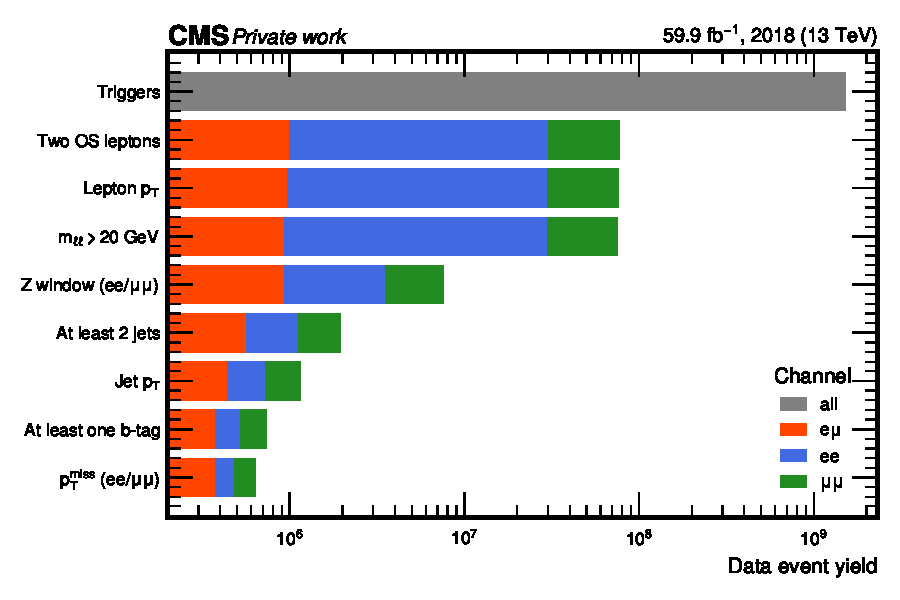
\includegraphics[width=\textwidth]{figures/ah/cutflows.pdf}
    \caption{\textbf{Selection cuts.} Shown is the data yield in 2018 (corresponding to $\Lint = \lumiVIII$) after successively applying all selection cuts. Starting with the requirement of two opposite-sign leptons, the three channels are marked with different colors.}
    \label{fig:ah:cutflows}
\end{figure}

\subsection{Experimental corrections}
\label{sec:ah:expcorrs}

Similar as in \cref{sec:ttxs:corrections}, several corrections are applied to the MC simulation in order to achieve good agreement with the data. In contrast to the \ttbar cross section measurement, where most of these corrections were derived as part of this work, many of the experimental corrections used in this chapter were provided centrally by the CMS collaboration. These will only be described very briefly; more details can be found in the associated references.

\paragraph{Trigger scale factors}

The selection efficiency of the triggers from \cref{tab:ah:triggers} needs to be corrected in simulation to the one measured in data. This is done via scale factors, which were centrally derived as a function of the \pt of the two leptons using the so-called cross-trigger method: Events are selected using a different set of triggers - here, a combination of jet and \ptmiss triggers - which is assumed to be fully orthogonal to the lepton triggers used for the main selection. Thus, the event sample is unbiased with respect to the lepton triggers, and the lepton trigger efficiency can be measured as the fraction of these events who pass the lepton triggers in addition to the jet/\ptmiss triggers. This is done independently for all data taking years, and the resulting scale factor differs from unity by less then 1 \% in most cases.

\paragraph{Lepton scale factors}

Differences in the efficiency for a lepton to pass the identification and isolation criteria as defined in \cref{sec:ah:objects} are measured using the tag-and-probe method, as in \cref{sec:ttxs:corrections}, and applied to simulation using scale factors binned in \pt and \abseta of the lepton. The scale factor typically differs from unity by about 1-5 \%, with the magnitude increasing for high \abseta. For more details on this method see Refs.~\cite{CMS:EGM-17-001,CMS:MUO-16-001}.

\paragraph{Pileup reweighting}

In contrast to the data-driven reweighting method used for the inclusive \ttbar cross section measurement (\cref{sec:ttxs:corrections}), the mean number of pileup interactions per bunch crossing in simulation is reweighted to year-dependent distributions provided centrally by CMS. These have been derived from measurements of the instantaneous luminosity combined with a total inelastic proton-proton cross section of $\SI{69.2}{\milli\barn} \pm 4.6 \%$ at \sqrtsRII~\cite{CMS:LUM-17-003}.


\paragraph{Jet energy corrections}

The difference in the jet energy response of the detector as well as the jet energy resolution in data and simulation was corrected in the same way as described in \cref{sec:ttxs:corrections}, using centrally derived jet energy corrections (JECs) as described in \citere{CMS:JME-13-004}.

\paragraph{b-tagging scale factors}

The identification efficiency of the \textsc{DeepJet} b-tagging algorithm was calibrated on events with jets containing a muon, which are likely to result from the semileptonic decay of a B hadron, using the methodology described in \citere{CMS:BTV-16-002}. Note that, unlike most CMS analyses using b-tagging, the calibration done on dileptonic \ttbar events presented in the same reference is not used as an input here, since it was derived in part on the same data set as used for this search, and would thus lead to double-counting. However, similar to the discussion in \cref{sec:ttxs:fitresults}, it is expected that the b-tagging efficiency will be constrained from the data during the likelihood fit.

\paragraph{ECAL L1 pre-firing}

In the 2016 and 2017 data-taking years, the L1 trigger of the electromagnetic calorimeter was affected by a gradual shift in the timing of the inputs in the forward region ($\abseta > 2.0$)~\cite{CMS:TRG-17-001}. This effect, called L1 pre-firing, is corrected for using simulation scale factors computed from data.

\paragraph{Z+jets background normalization}

In the same-flavor lepton channels (\ee and \mumu), Z+jets events again constitute a minor but important background. Since this analysis is sensitive to small shape effects, it is necessary to precisely model this background both in shape and normalization. An NNLO Monte Carlo simulation (see \cref{tab:ah:simulation}) is used for this purpose, which generates up to two partons (including b quarks) in the final state, as required by the event selection of at least two jets and at least one b tag. Still, in order to be certain of the Z+jets rate, the same data-driven estimation as presented in \cref{sec:ttxs:datadriven}, using a control region with $|\mll - m_Z| < \SI{15}{\GeV}$ and a sideband with zero b-tagged jets, is performed. The resulting ratios of Z+jets yields compared to the prediction of the original simulation can be found in \cref{tab:ah:dysf}.

\begin{table}
    \begin{centering}
    \begin{tabular}{c|c|c|c|c}
     & 2016pre & 2016post & 2017 & 2018\tabularnewline
    \hline
    \hline
    \ee & $0.96\pm0.010$ & $0.97\pm0.008$ & $0.87\pm0.006$ & $0.88\pm0.005$\tabularnewline
    \hline 
    \emu & $0.96\pm0.007$ & $0.97\pm0.005$ & $0.88\pm0.004$ & $0.89\pm0.003$\tabularnewline
    \hline 
    \mumu & $0.96\pm0.009$ & $0.97\pm0.006$ & $0.90\pm0.005$ & $0.90\pm0.004$
    \end{tabular}
    \par\end{centering}
    \caption{\textbf{Z+jets scale factors.} Ratio of the Z+jets event yields estimated in data using the method described in \cref{sec:ttxs:datadriven} to the prediction by the MC simulation for the four data-taking periods. The results in the \emu channel are the geometric means of those in the \ee and \mumu channels. Uncertainties are statistical only.}
    \label{tab:ah:dysf}
\end{table}
    

\subsection{Reconstruction of the \ttbartitle system}
\label{sec:ah:kinreco}

Having identified the relevant objects - leptons, jets and \ptmissvec - in an event, the next step consists of reconstructing the \ttbar system, i.e. the four-momenta of the top and antitop quark. Due to the presence of the two neutrinos in the dileptonic \ttbar decay, which escape the detector unobserved except for \ptmissvec and thus represent a loss of information, this is a non-trivial procedure which requires several assumptions on the kinematic properties. In this work, a variation of the algorithm first presented in \citere{CMS:TOP-12-028} is used, which is briefly outlined in this section.

The algorithm works in two steps, starting with the assignment of jets to the b and \bbar quarks originating from the \ttbar decay. To do so, pairs of jets are selected from all jets in the event (passing the requirements outlined in \cref{sec:ah:objects}) depending on the number $n_b$ of b-tagged jets: For events with $n_b \geq 2$, all (ordered) permutations of two b-tagged jets each are considered as candidate pairs, while for events with $n_b = 1$, the candidate pairs are formed by pairing the single b-tagged jet with all other jets in the event. 

From these candidates, the best pair is now chosen based on the invariant masses $m_{\ell^+ b}$ and $m_{\ell^- \bar{b}}$ of the b/\bbar candidate and the corresponding (anti)lepton. In each event, the candidate pair is chosen that maximizes the product of the truth-level likelihoods, as evaluated from MC events, to obtain the measured values of $m_{\ell^+ b}$ and $m_{\ell^- \bar{b}}$. This pair is then used for the remainder of the reconstruction.
%As a result, the number of such $b \bar{b}$ candidate pairs in an event will be $n_{\mathrm{cand}} = n_b (n_b - 1)$ for events with at least two b-tagged jets and $n_{\mathrm{cand}} = 2 n_l$ for events with one b-tagged jet. Here, $n_b$ and $n_l$ are the number of b-tagged and non-btagged jets in the event, respectively. 

Next, the four-momenta of the top and antitop quark are reconstructed using the momentum conservation equations. That is, one demands

\begin{equation}
\begin{split}
    p_t &= p_{W^+} + p_{b} = p_{\ell^+} + p_{\nu_{\ell}} + p_{b} \\
    p_{\bar{t}} &= p_{W^-} + p_{\bar{b}} = p_{\ell^-} + p_{\bar{\nu}_{\ell}} + p_{\bar{b}}
\end{split}
\end{equation}

where all variables are understood as four-momenta. The lepton and b-quark momenta are experimentally measured, while the neutrino momenta are unknowns. Demanding them to be massless, i.e. $p_{\nu_{\ell}}^2 = p_{\bar{\nu}_{\ell}}^2 = 0$, yields the six components of the two neutrino three-momenta as free parameters.

To resolve the ambiguities, several assumptions need to be made. First, it is assumed that all of the missing transverse momentum in the event stems from the neutrinos, i.e.

\begin{equation}
    p_{\nu_{\ell},x} + p_{\bar{\nu}_{\ell},x} = p_{x}^{\mathrm{miss}} , \quad p_{\nu_{\ell},y} + p_{\bar{\nu}_{\ell},y} = p_{y}^{\mathrm{miss}}
\end{equation}

Additionally, it is assumed that both the top quarks and W bosons are exactly on-shell, that is

\begin{equation}
    p_{W^+}^2 = m_W^2 , \quad p_{W^-}^2 = m_W^2
\end{equation}

and

\begin{equation}
    p_{t}^2 = m_t^2 , \quad p_{\bar{t}}^2 = m_t^2
\end{equation}

where $m_t$ and $m_W$ are the pole masses of the top quark and W boson, respectively. Applying these six constraints leads to a system of quartic equations for the neutrino three-momenta $\vec{p}_{\nu_{\ell}}$ and $\vec{p}_{\bar{\nu}_{\ell}}$, which was solved in \citere{Sonnenschein:2006ud}. From these, the top and antitop quark four-momenta can then be calculated. Since the quartic equation can in general have up to four solutions, the solution with the lowest value of the invariant \ttbar mass \mtt is chosen. This was found in \citere{Korol:2016wzq} to minimize the bias in \mtt especially for low-\mtt events.

In practice, however, this method will not give a real solution even for those \bbbar pair candidates which are correctly assigned to the truth-level b quarks. This is because the experimental inputs to the method - the jet and lepton four-momenta as well as \ptmissvec - will deviate from their truth-level values within the experimental resolution of the detectors and object reconstruction. In addition, the constraints will not be fulfilled exactly: There might be additional \ptmiss in the event because of e.g. neutrinos produced in $\tau$ lepton or B hadron decays, and the W bosons and top quarks might be off-shell with respect to their pole masses by their respective widths.

To alleviate this, several of the input variables are randomly smeared to model the experimental resolution. For both the b jets and leptons, the energies are varied while keeping their masses constant, and the directions of their three-momenta are varied in a uniformly random direction. For both of these cases, the variations are randomly sampled from a distribution obtained by comparing the reconstructed and truth four-momentum in the nominal \ttbar MC simulation, as shown in \citere{Rubenach:PhD}. Additionally, the values of $m_W$ used for the constraints on $p_{W^+}$ and $p_{W^-}$ are randomly sampled from a relativistic Breit-Wigner distribution corresponding to the W boson width $\Gamma_W$. This smearing procedure is repeated 100 times per event with different random values, resulting in up to 100 reconstructed \ttbar systems per event, depending on the number of cases where there is no real solution. %Combined with the $n_{\mathrm{cand}}$ possible $b \bar{b}$ assignments, this results in $100 n_{\mathrm{cand}}$ reconstructed \ttbar systems per event, of which not all might have real solutions.

Finally, one unambiguous solution per event is constructed by again using the invariant lepton-b quark masses and their truth-level likelihoods. 
For each iteration of the smearing procedure that yielded a real solution, a weight is defined as the product of the likelihoods for obtaining the smeared values of $m_{\ell^+ b}$ and $m_{\ell^- \bar{b}}$, i.e.
%To finally construct one unambiguous solution per event, the invariant lepton-b quark masses $m_{\ell^+ b}$ and $m_{\ell^- \bar{b}}$ are calculated for each real solution and compared to their expected truth-level distributions, evaluated again in the nominal \ttbar simulation. A weight is constructed as the product of the truth-level probabilities to obtain the given $m_{\ell^+ b}$ and $m_{\ell^- \bar{b}}$ values, i.e.

\begin{equation}
\label{eq:ah:kinrecoweight}
    w = \mathcal{P} (m_{\ell^+ b}) \cdot \mathcal{P} (m_{\ell^- \bar{b}})
\end{equation}

The final solution for the reconstructed top and antitop four-momenta is defined as the weighted average over all real solutions, using the weight as given in \cref{eq:ah:kinrecoweight}.

\begin{figure}[t]
    \centering
    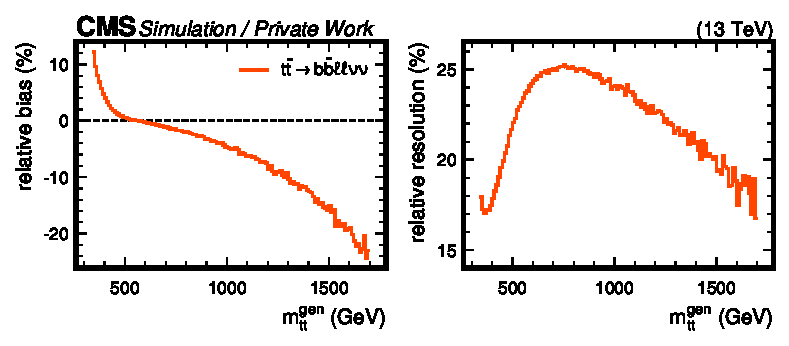
\includegraphics[width=0.99\linewidth]{figures/ah/mtt_resolution.pdf}
    \caption{\textbf{Bias and resolution of \mtt.} Relative bias and resolution of the \ttbar reconstruction algorithm, defined in \cref{eq:ah:deltamtt}, as a function of truth-level \mtt and evaluated in MC simulation of dileptonic \ttbar.}
    \label{fig:ah:resolution}
\end{figure}

For $\ttbar \rightarrow \bbllnunu$ events passing all previous selection steps, the efficiency of the full reconstruction algorithm is ca. $90\%$, as evaluated in MC simulation. To asses the accuracy of the reconstruction relative to the truth-level top quarks, defined after parton showering, a per-event relative deviation is defined as 

\begin{equation}
\label{eq:ah:deltamtt}
    \Delta \mtt = \frac{\mtt^{\mathrm{reco}} - \mtt^{\mathrm{gen}}} {\mtt^{\mathrm{gen}}},
\end{equation}

\noindent where $\mtt^{\mathrm{reco}}$ and $\mtt^{\mathrm{gen}}$ stand for the reconstructed and truth-level \mtt, respectively. The mean and standard deviation of $\Delta \mtt$ are then the relative bias and resolution of the reconstruction algorithm. They are evaluated in simulation of dileptonic \ttbar and shown in \cref{fig:ah:resolution} as a function of truth-level \mtt. The method shows a bias towards high \mtt for events with $\mtt^{\mathrm{gen}} \lesssim \SI{600}{\GeV}$ and towards low \mtt for $\mtt^{\mathrm{gen}} \gtrsim \SI{600}{\GeV}$, with resolutions in the range of $17-25\%$. It should be noted here that this bias relative to the truth level is by itself not problematic for this analysis, since it is expected to be the same in both simulation and data and no unfolding of the reconstructed distributions to the truth level is attempted here.

\subsection{Sensitive observables}

To extract the A/H and \etat signals from the background, three sensitive observables are considered. The first is simply the invariant \ttbar mass \mtt, defined with the reconstruction procedure as explained in the last section. As shown in \cref{fig:theory:ahxs}, an A/H signal is expected to result in a peak-dip structure in \mtt around the SM background, where the zero crossing between peak and dip should be in the vicinity of the A/H mass, and the magnitude as well as ratio of the peak and the dip depends non-linearly on the coupling modifier. The \etat signal, on the other hand, is expected to peak slightly below the \ttbar production threshold at $\mtt \simeq 2 \mt - \SI{2}{GeV}$ as discussed in \cref{sec:theory:etat} and shown in \cref{fig:theory:etat}. In practice, due to the limited detector resolution, the exact position of this peak will not be observable, and the signal will result in a generic enhancement of the yield for very low values of \mtt.

In addition, the two spin correlation observables \chel and \chan, as defined in \cref{eq:theory:cheldef} and \cref{eq:theory:chan}, are used to gain further sensitivity. Both variables are again defined using the \ttbar system reconstruction as described in the previous section. As discussed in \cref{sec:theory:spindensity}, they are ideal for separating spin-singlet and spin-triplet states, respectively. Thus, A and \etat signals, producing singlet states, will have enhanced contributions at high values of \chel, while H signals, producing \term{3}{P}{0} triplet states, will be enhanced at low values of \chan. This allows not only for better discrimination between signal and background, but also to probe the \CP structure of a possible observed signal. 

\begin{figure}[t]
    \centering
    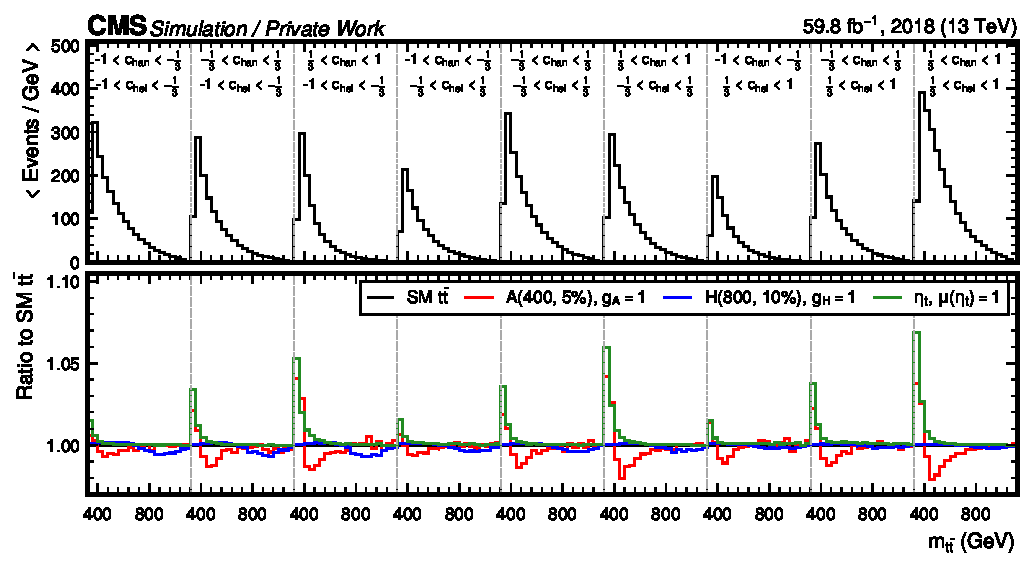
\includegraphics[width=0.99\linewidth]{figures/ah/mttchelchan.pdf}
    \caption{\textbf{3D template for \mttchelchan} for SM \ttbar (top) as well as three different example signals (bottom, shown as the ratio to SM \ttbar), corresponding to the luminosity taken in 2018 only.}
    \label{fig:ah:mttchelchan}
\end{figure}


To combine all three variables, three-dimensional templates are created with $20 \times 3 \times 3$ bins in the three observables \mtt, \chel and \chan. For \mtt, an irregular binning is chosen to account for the decrease in production cross section at high values. An example can be seen in \cref{fig:ah:mttchelchan} for SM \ttbar and three different signals (A, H and \etat).

\section{Higher-order corrections in \ttbartitle}
\label{sec:ah:ttbarweights}

In this analysis, the SM \ttbar background is irreducible - after all, it leads to the exact same final state as the signal. As a result, it is crucial to model it as precisely as possible: a mismodeling of the \ttbar kinematic distribution, especially in \mtt, might otherwise be confused for a signal and lead to bias.

The MC simulation used for the SM \ttbar background is performed at NLO in QCD using the \powhegvtwo subprocess \hvq, as studied also in \cref{ch:bb4l}. On top of this, two different sets of corrections are applied to include missing higher orders, namely NNLO QCD and NLO electroweak (EW) corrections. Both of these are estimated by comparing the MC simulation, which is matched to a parton shower, to fixed-order predictions. The simulation is then reweighted using scale factors binned two-dimensionally in \mtt and $\cost_t$, where the latter is the cosine of the scattering angle of the top quark to the beam axis in the \ttbar rest frame. These two variables fully define the kinematics of the top quarks in the \ttbar rest frame, save for FSR emissions.%In the SM, this variable is strongly correlated with the observables \chel and \chan, and is thus used in their place since spin correlation observables cannot be defined in calculations at stable top level.

\subsection{NNLO QCD corrections}

The NNLO QCD predictions are obtained with the program MATRIX~\cite{Grazzini:2017mhc}. They are computed at the level of stable top quarks with a dynamic scale choice of $\sqrt{\smash[b]{\mt^2+p_{T,t}^2}}$, where $p_{T,t}$ is the top quark transverse momentum. \cref{fig:ah:ewqcdcorrs} shows the resulting effect on the 3D \mttchelchan distribution at the detector level as the black line. They are on the order of $1-2\%$.

\begin{figure}[t]
    \centering
    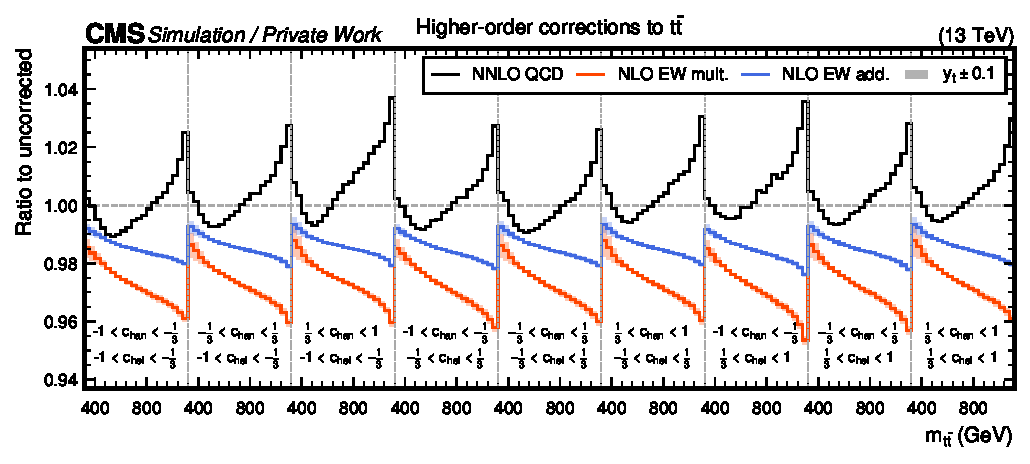
\includegraphics[width=0.99\linewidth]{figures/ah/ewqcdcorrs.pdf}
    \caption{\textbf{Effect of NNLO QCD and NLO EW corrections} on the 3D \mttchelchan distribution after reconstruction in the form of ratios to the uncorrected distributions. The NNLO QCD corrections are shown as the solid black line, while the NLO EW corrections are shown in orange for the multiplicative scheme and in blue for the additive scheme. The effect of varying \yt by $\pm 0.1$ in the NLO EW corrections is shown as the shaded bands.}
    \label{fig:ah:ewqcdcorrs}
\end{figure}

\subsection{NLO EW corrections}
\label{sec:ah:ewcorr}

\begin{figure}[t]
    \centering
    \begin{tikzpicture}
      \begin{feynman}
        \vertex (i1) {\(g\)};
        \vertex [below=2.0 cm of i1] (i2) {\(g\)};
        \vertex [right=1.5 cm of i1] (a);
        \vertex [right=1.5 cm of i2] (b);
        \vertex [right=1.5 cm of a] (c);
        \vertex [right=1.5 cm of b] (d);
        \vertex [right=1.5 cm of c] (f1) {\(t\)};
        \vertex [right=1.5 cm of d] (f2) {\(\bar{t}\)};
        \diagram* {
          (i1) -- [gluon] (a),
          (i2) -- [gluon] (b),
          (c) -- [scalar, edge label=\(h\)] (d),
          (f1) -- [anti fermion] (c) -- [anti fermion] (a) -- [anti fermion, edge label=\(t\)] (b) -- [anti fermion] (d) -- [anti fermion] (f2)
        };
      \end{feynman}
    \end{tikzpicture}
    \caption{\textbf{EW correction involving a SM Higgs boson.} An example Feynman diagram for NLO EW corrections to \ttbar production involving the exchange of a virtual SM Higgs boson $h$.}
    \label{fig:ah:ewcorr_feynman}
\end{figure}

The NLO corrections in the electroweak coupling \alphaew are computed with the HATHOR code~\cite{Aliev:2010zk, Kuhn:2005it, Kuhn:2006vh, Kuhn:2013zoa} using the same nominal scale choices. Of particular interest here is a class of diagrams which contain an exchange of a virtual SM Higgs boson, an example of which is seen in \cref{fig:ah:ewcorr_feynman}. The matrix element for this diagram is proportional to the square of the SM Higgs-top Yukawa coupling \yt, giving a $\yt^2$-dependent correction to \ttbar distributions from the interference with LO diagrams. This correction is sizable mostly for low \mtt values, and is important for this analysis because the SM Higgs exchange might change the \ttbar spin state and thus \chel and \chan. To accurately account for this, the correction is derived separately for the different initial states ($gg$, $q\bar{q}$ and $gq$) of \ttbar production.

The results obtained with HATHOR are accurate only to LO in \alphas, i.e. \order{\alphas^2}, and as of the time of writing no full calculation including both NLO QCD and EW effects exists. Thus, there is an ambiguity on how the NLO-accurate (in QCD) MC simulation and the NNLO-accurate corrections presented in the previous section should be combined with the EW corrections.

Formally, the differential cross section as predicted by Powheg can be decomposed as

\begin{equation}
    d \sigma_{\powheg} = \alphas^2 d \sigma_{\mathrm{LO}} + \alphas^3 d \sigma_{\mathrm{NLO}}
\end{equation}

\noindent where additional terms beyond $\order{\alphas^3}$ due to additional radiation in Powheg and Pythia are not written for simplicity. On the other hand, HATHOR predicts

\begin{equation}
    d \sigma_{\mathrm{HATHOR}} = \alphas^2 d \sigma_{\mathrm{LO}} + \alphas^2 \alphaew d \sigma_{\mathrm{EW}}.
\end{equation}

One possible way to combine the calculations is the additive scheme, given by


\begin{equation}
\begin{split}
\label{eq:ah:ewadd}
    d \sigma_{\mathrm{add.}} &= d \sigma_{\powheg} + d \sigma_{\mathrm{HATHOR}} - \alphas^2 d \sigma_{\mathrm{LO}} \\
    &= \alphas^2 d \sigma_{\mathrm{LO}} + \alphas^3 d \sigma_{\mathrm{NLO}} + \alphas^2 \alphaew d \sigma_{\mathrm{EW}}
\end{split}
\end{equation}

\noindent which is formally accurate to $\order{\alphas^3}$ and $\order{\alphas^2 \alphaew}$. This approach does not include any cross terms of order $\order{\alphas^3 \alphaew}$, which are not fully calculated by either Powheg or HATHOR. However, it is reasonable to assume that these cross terms factorize approximately, leading to the alternative multiplicative scheme~\cite{Kuhn:2013zoa}

\begin{equation}
\begin{split}
\label{eq:ah:ewmult}
    d \sigma_{\mathrm{mult.}} &= d \sigma_{\powheg} \times \frac{d \sigma_{\mathrm{HATHOR}}} {\alphas^2 d \sigma_{\mathrm{LO}}} \\
    &= \alphas^2 d \sigma_{\mathrm{LO}} + \alphas^3 d \sigma_{\mathrm{NLO}} + \alphas^2 \alphaew d \sigma_{\mathrm{EW}} + \alphas^3 \alphaew \frac {d \sigma_{\mathrm{NLO}} \, d \sigma_{\mathrm{EW}}}{d \sigma_{\mathrm{LO}}}
\end{split}
\end{equation}

The difference between the two schemes is in the last term of order $\order{\alphas^3\alphaew}$, which is an approximation to the QCD-EW cross terms. In this work, the multiplicative approach is used for all nominal results, while the difference to the additive approach is included as a systematic uncertainty. In both cases, the needed term $\alphas^2 d \sigma_{\mathrm{LO}}$ is computed with \madgraph.

The effect of both approaches on the 3D \mttchelchan distribution at the detector level after parton showering can be seen in \cref{fig:ah:ewqcdcorrs} for different values of \yt. The multiplicative scheme leads to a larger correction of roughly $2-4\%$, while the additive scheme only gives $1-2\%$. Notably, the effect of varying \yt modifies not only the \mtt distribution close to the \ttbar threshold, but also the distribution of \chel. As a result, such a variation in data could potentially be confused for a pseudoscalar signal. It is thus important to include it as a systematic uncertainty, as described in \cref{sec:ah:systs}.


\section{Matrix element reweighting for \AH signals}
\label{sec:ah:mereweighting}

In order to probe the full phase space of the generic \AH model as described in \cref{sec:ah:intro}, predictions at different \AH masses and widths with a sufficiently small spacing are required so that interpolation between the points is possible. However, generating a separate MC sample for each mass and width point is computationally very expensive.

\subsection{Principle of the method}

As an alternative, it is possible to re-use existing samples for different mass and width points via matrix element reweighting. This method works by noting that a given MC sample can be seen as a random sample, drawn from a PDF of the form

\begin{equation}
\label{eq:ah:merewprob}
    \mathcal{P}(x_i^{\mathrm{ME}}, x_j^{\mathrm{reco}}) = \mathcal{P}^{\mathrm{ME}} (x_i^{\mathrm{ME}}) \cdot \mathcal{P}^{\mathrm{rem}} (x_j^{\mathrm{reco}} | x_i^{\mathrm{ME}})
\end{equation}

Here, $x_i^{\mathrm{ME}}$ are all variables defining the event at the matrix element (ME) level, i.e. at the level of the hard interaction, and $x_j^{\mathrm{reco}}$ are all variables after detector simulation and object reconstruction. For the case of the \AH signals, which are generated at LO in QCD, $x_i^{\mathrm{ME}}$ is given fully by the four-momenta and helicities of the final-state particles (leptons, neutrinos and b quarks) in the hard process. The $x_j^{\mathrm{reco}}$ consist of all possible reconstruction-level variables that are relevant to the analysis, such as e.g. jet and lepton four-momenta, lepton identification criteria or \ptmissvec. 

$\mathcal{P}^{\mathrm{ME}} (x_i^{\mathrm{ME}})$ refers to the probability density of the ME-level variables as predicted by the ME generator, which will be proportional to the absolute square of the matrix element. This function will depend on the chosen scenario of the \AH model, i.e. $m_{\AH}$ and $\Gamma_{\AH}$. Meanwhile, the conditional probability density $\mathcal{P}^{\mathrm{rem}} (x_j^{\mathrm{reco}} | x_i^{\mathrm{ME}})$ encodes the effects of all other components of the simulation chain, such as the parton shower, hadronization, detector simulation and reconstruction. It gives the probability to observe reconstruction-level variables $x_j^{\mathrm{reco}}$ for an event with ME-level variables $x_i^{\mathrm{ME}}$.

The principal assumption of the method is now that $\mathcal{P}^{\mathrm{rem}}$, and thus the whole simulation chain except for the matrix element, is independent of the underlying \AH signal scenario ($m_{\AH}$ and $\Gamma_{\AH}$). This assumption is certainly true for the detector simulation and reconstruction, while care must be taken for the parton shower, which in general needs to be matched to the matrix element and can this way have a residual dependence. The validity of the assumption will be discussed in more detail below.

If the assumption is fulfilled, a given \AH MC sample generated with parameters $m_{\AH}^0$ and $\Gamma_{\AH}^0$ can now be reweighted to a different \AH scenario with parameters $\hat{m}_{\AH}$ and $\hat{\Gamma}_{\AH}$ by applying to each event $i$ a weight 

\begin{equation}
\label{eq:ah:merewweight}
    w_i = \frac{ \mathcal{P}^{\mathrm{ME}} (x_i^{\mathrm{ME}} | \hat{m}_{\AH} , \hat{\Gamma}_{\AH} ) } { \mathcal{P}^{\mathrm{ME}} (x_i^{\mathrm{ME}} | m_{\AH}^0 , \Gamma_{\AH}^0 ) }
\end{equation}

The quantities in the denominator and nominator are the ME-level probability densities for each event, evaluated at the original and target \AH parameters, respectively. When this weight is inserted into \cref{eq:ah:merewprob}, the original probability cancels, giving the correct probability density for the target scenario $\hat{m}_{\AH}$ and $\hat{\Gamma}_{\AH}$.

In practice, this method will only work if the MC sample used for the reweighting has sufficient phase space overlap with the target \AH scenario, i.e. if the two probabilities in \cref{eq:ah:merewweight} are not too different from each other for the majority of the events. Otherwise, the weights will become very small in some regions of the phase space and very large in others, resulting in poor statistics for the reweighted sample.

The method was implemented by directly evaluating the squared matrix elements for the different \AH hypotheses, using the standalone reweighting interface provided by \madgraph and the same UFO model as for the signal generation. 

\subsection{Combination of multiple origin samples}

For the purpose of this analysis, a set of signal samples for different \AH scenarios (as given in \cref{sec:ah:datasets}) was already available at the time of starting these studies. These samples were used as origin samples for the reweighting. In order to maximize the statistics achieved after reweighting for each target \AH scenario, and mitigate problems from poor phase space overlap, a subset of the available samples were combined after reweighting for each target scenario.

This procedure works as follows: First, a set of several origin samples $j$ with different parameters $m_{\AH}$ and $\Gamma_{\AH}$ are all reweighted separately to the same target parameters $\hat{m}_{\AH}$ and $\hat{\Gamma}_{\AH}$ with per-event weights $w_{i,j}$ as given in \cref{eq:ah:merewweight}. These need to be multplied with a possible generator weight of the origin sample $u_{i,j}$, giving the total per-event weight $\hat{w}_{i,j} = w_{i,j} u_{i,j}$. For fully unweighted origin samples, $u_{i,j} = 1$. 

Then, the different samples are again weighted with a per-sample weight $v_j$ proportional to

\begin{equation}
\label{eq:ah:sampleweights}
    v_j \propto {\langle \hat{w}_{i,j} \rangle}^{-1} =  \frac{ \sum_i \hat{w}_{i,j} }{ \sum_i \hat{w}_{i,j}^2 }
\end{equation}

\noindent where the sums run over all events $i$ in the considered sample $j$. This expression is the inverse of the average ME weight for sample $j$. It is chosen such that samples with large phase space overlap with the target \AH scenario - and thus small ME weights $w_{i,j}$ - are assigned a large weight $v_j$ in the combination of samples. Similarly, samples with poor phase space overlap, and thus large average ME weights, get assigned small weights and contribute less strongly to the combined sample. Finally, the total combined sample is normalized to the expected cross section for the target scenario, which is calculated independently. It is shown in App.~\ref{app:mereweighting} that this procedure minimizes the total statistical error of the combined sample.

In practice, all available masses and parities (A and H) are combined for each target \AH mass. Resonance and interference contributions are treated separately from each other. Furthermore, it was found that, for the resonance contribution only, it is necessary to split the combination of different \AH widths into two halves: those with $\wAH/\mAH$ less or greater than 10\%. This is due to an interplay of \madgraph and the \pythia shower leading to a dependency on the \AH width in the matrix element, which is not taken into account in the reweighting. For $\wAH/\mAH < 10\%$ (narrow resonance), \madgraph includes the intermediate \AH particle in the event record, which is then treated by \pythia as a unstable resonance and its virtuality as predicted by the matrix element is preserved. For $\wAH/\mAH \geq 10\%$ (broad resonance), the \AH particle is not included in the event record, and its virtuality is thus not preserved. This leads to slight differences in distributions affected by the parton showering. The choice of 10\% for the transition between the two modes is an arbitrary parameter, and thus not necessarily physical. Nonetheless, it was decided in this analysis to not mix the two width ranges in the reweighting in order to obtain full closure with a standalone generation.

\subsection{Validation}

The combined reweighting is validated for three masses of $\mAH = 400$, 600 and 800 GeV as well as widths of 2.5 and 10\%. For each of these points, the reweighting is performed as stated above, but leaving out \AH scenarios with the same mass from the combination of origin samples since otherwise the weights would be trivially one. The reweighted \mtt distributions at generator level are then compared to the standalone samples at the same \mAH and \wAH.

The resulting comparisons and residuals can be seen in \cref{fig:ah:merew_validation} for A and H, separated into the resonance and interference contributions. It can be seen that the closure between reweighting and standalone generation is excellent within the statistical uncertainties.

\begin{figure}[!p]
    \centering
    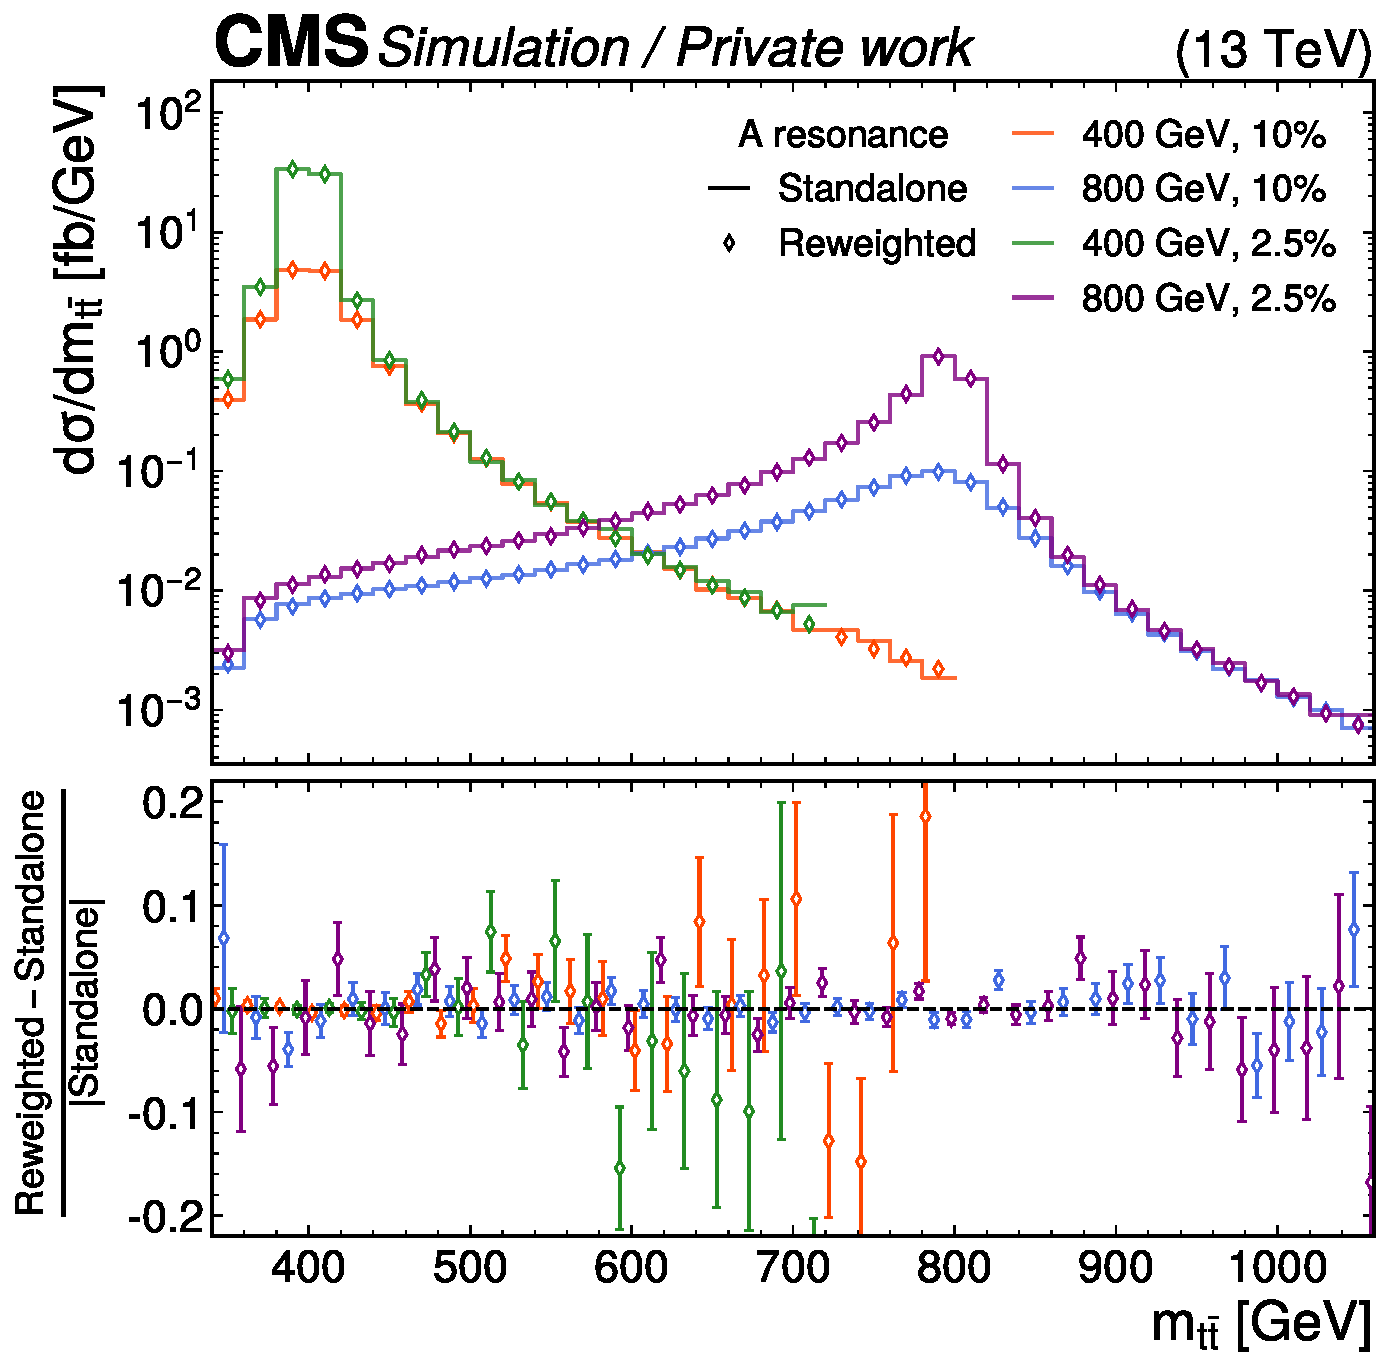
\includegraphics[width=0.49\textwidth]{figures/ah/me_reweighting/A_res.pdf}
    \hfill
    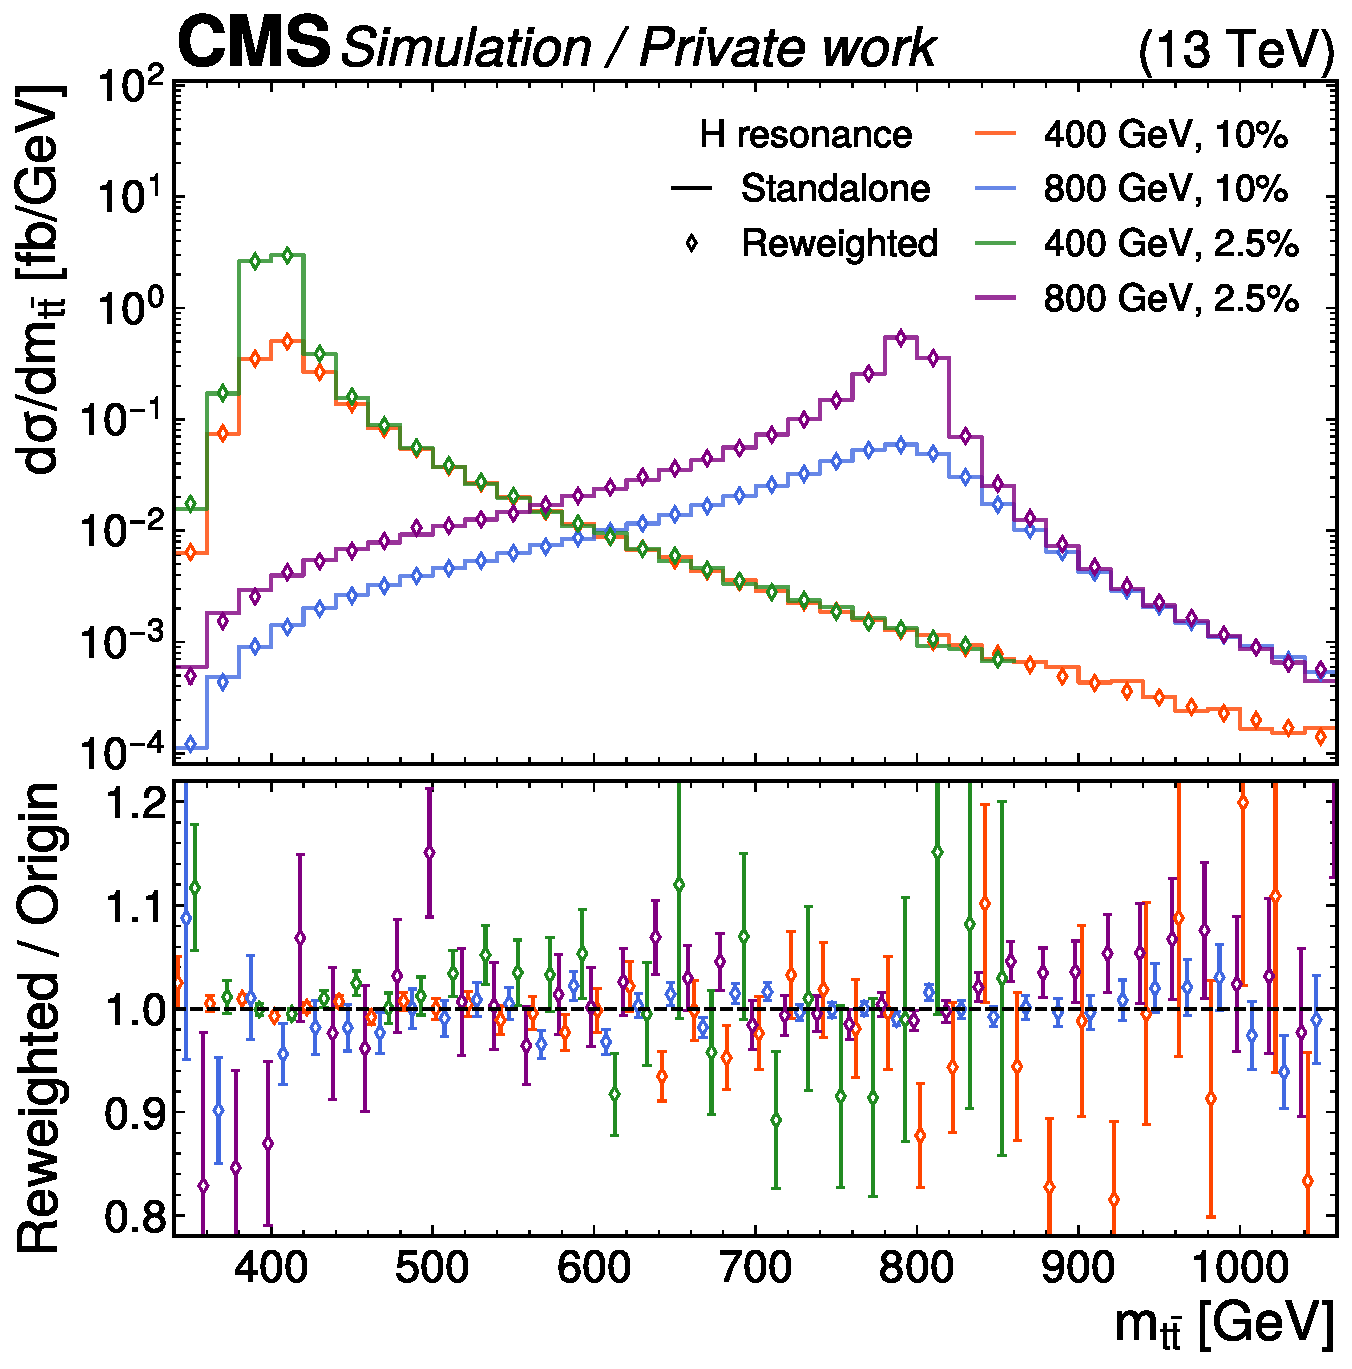
\includegraphics[width=0.49\textwidth]{figures/ah/me_reweighting/H_res.pdf}
    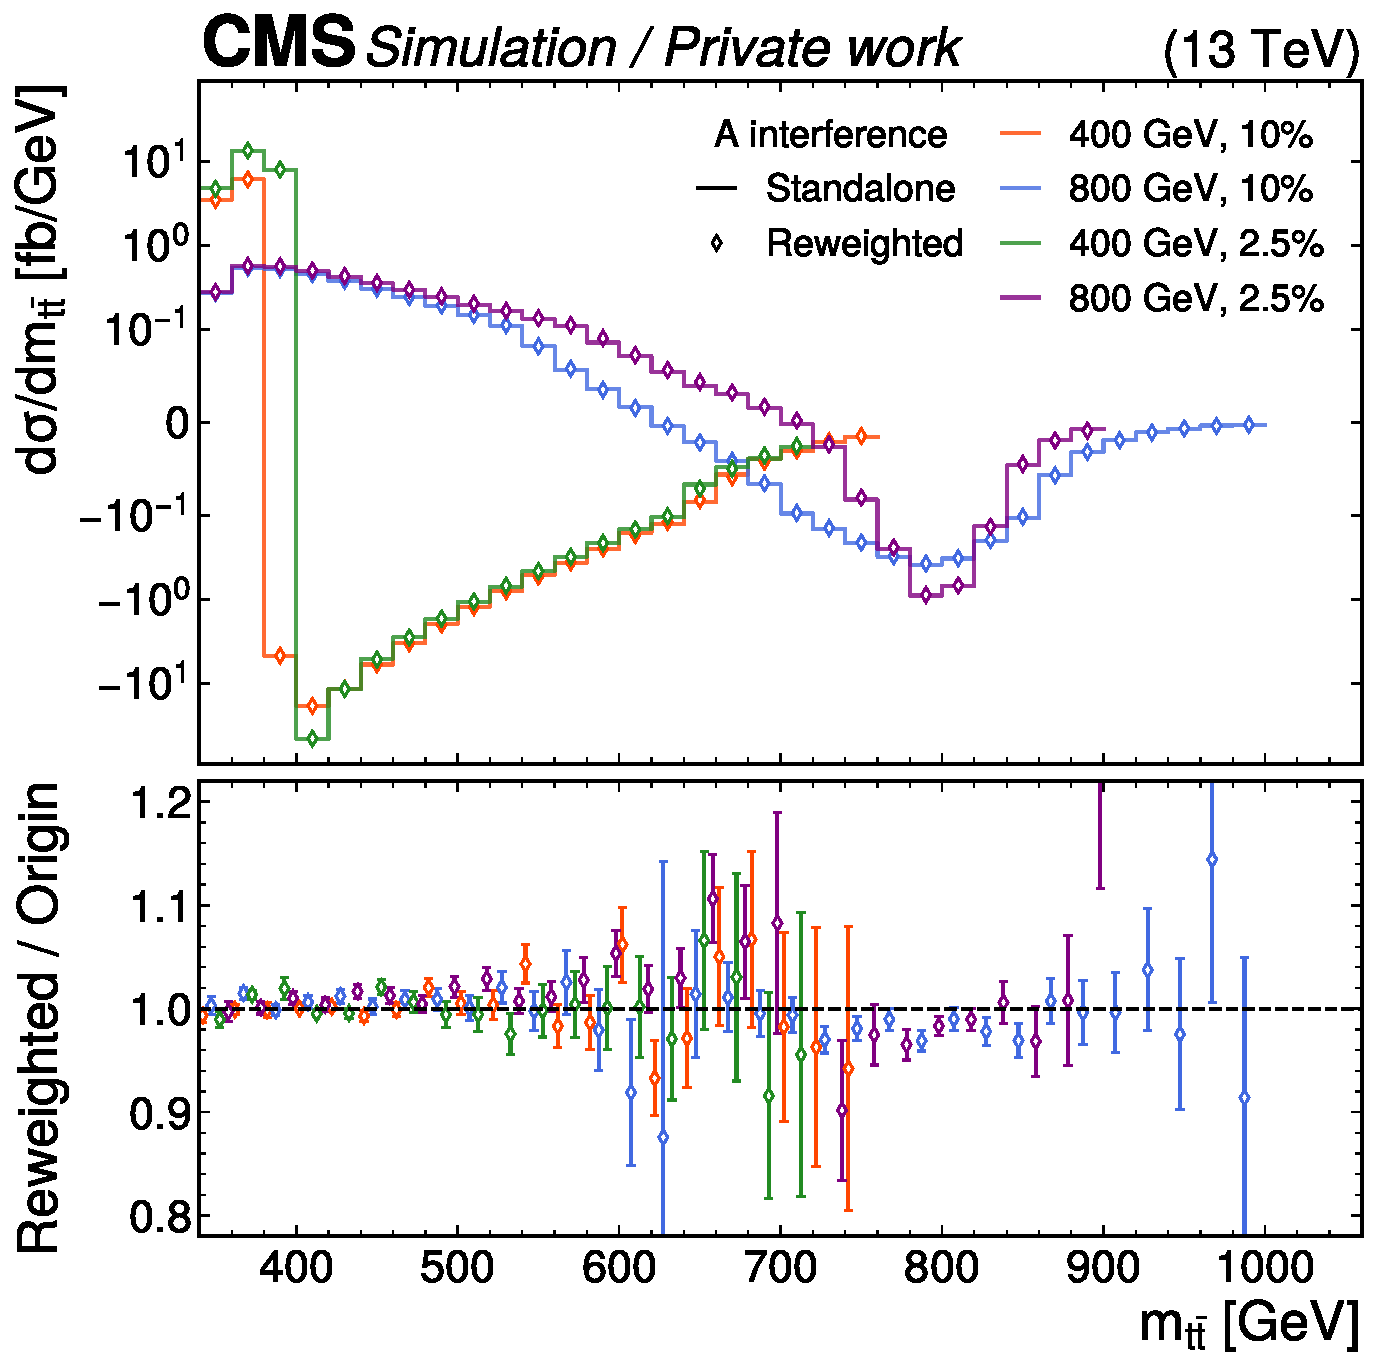
\includegraphics[width=0.49\textwidth]{figures/ah/me_reweighting/A_int.pdf}
    \hfill
    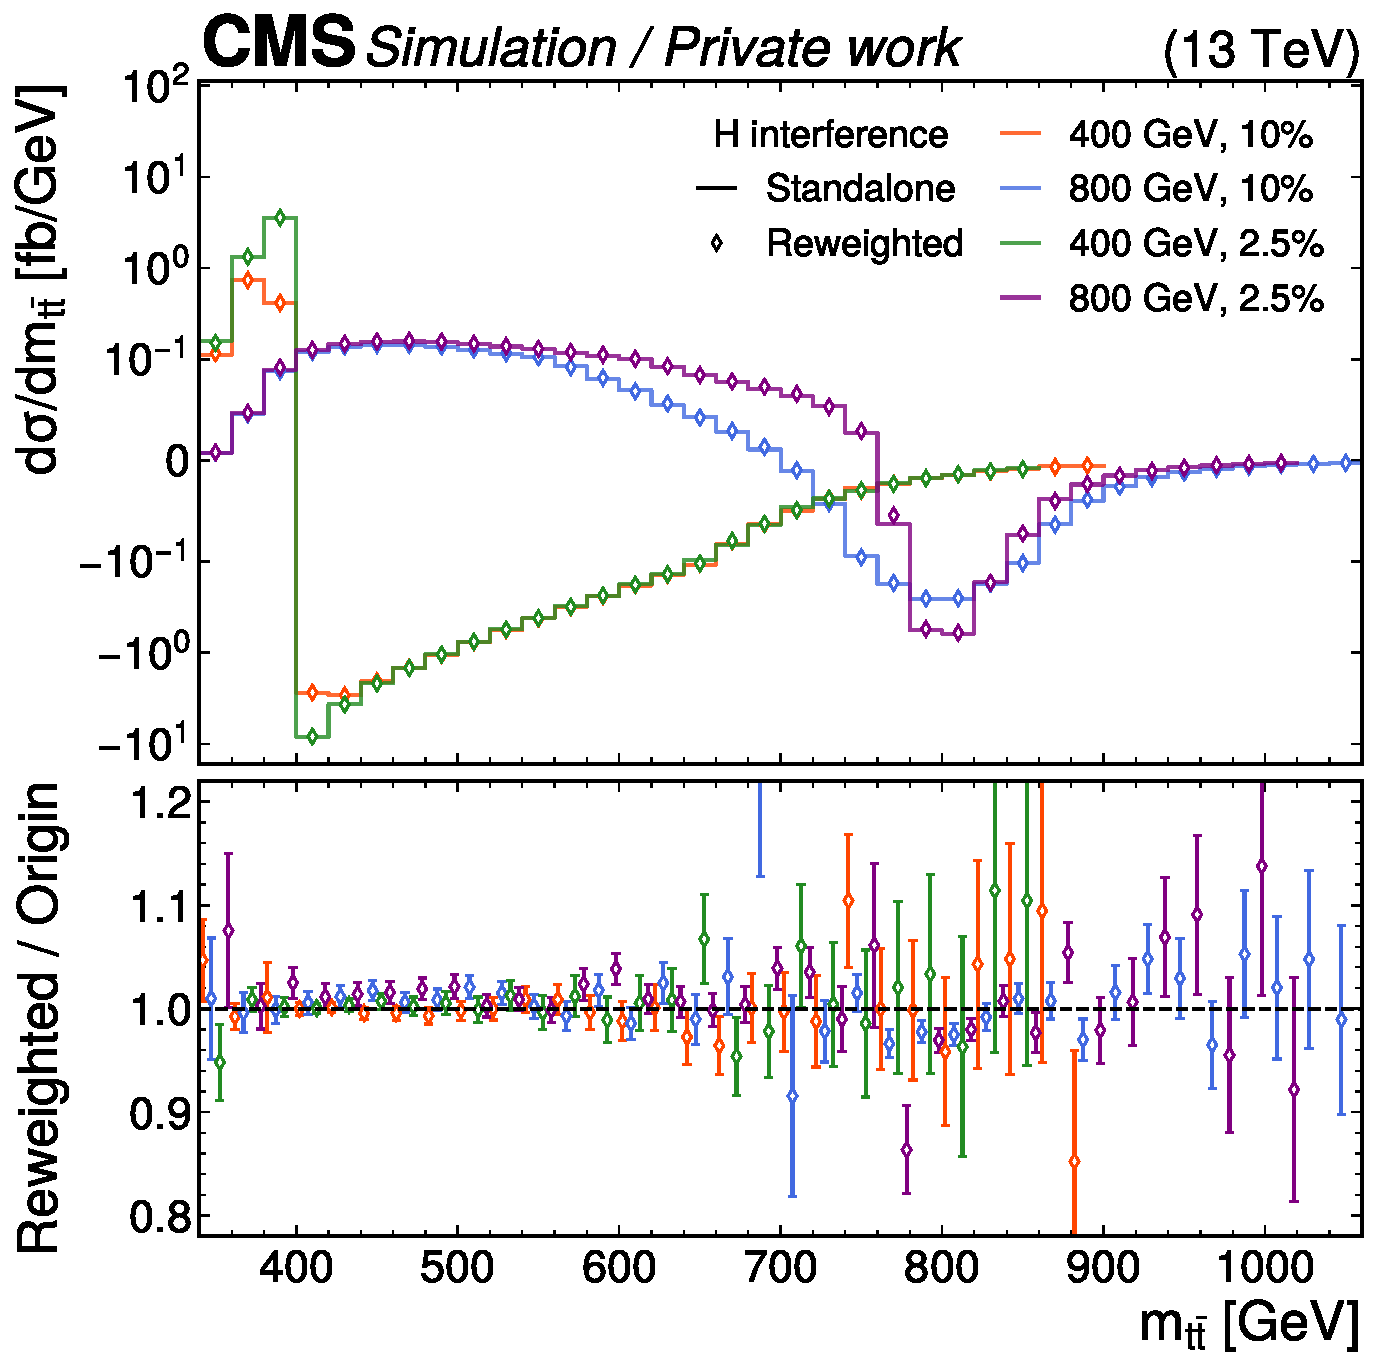
\includegraphics[width=0.49\textwidth]{figures/ah/me_reweighting/H_int.pdf}
    \caption{\textbf{Validation of the ME reweighting.} Comparison of standalone generated (lines) and reweighted (diamond markers) \mtt distributions for different values of \mAH and \wAH. From top left to bottom right: A resonance, H resonance, A interference, H interference. The lower panel shows the ratio of reweighted and standalone distributions. The error bars give the combined statistical uncertainty of the reweighted and standalone sample.}
    \label{fig:ah:merew_validation}
\end{figure}

\section{Systematic uncertainties}
\label{sec:ah:systs}

Similar to \cref{sec:ttxs:systematics}, systematic uncertainties affect the distributions of both SM background and signal processes. They are listed in this section, split into theory (\cref{sec:ah:theorysysts}) and experimental uncertainties (\cref{sec:ah:expsysts}).

\subsection{Theory uncertainties}
\label{sec:ah:theorysysts}

\paragraph{Scale uncertainties}
Uncertainties due to missing higher orders in the matrix element as well as the parton shower are included separately for the SM \ttbar, tW, and \Zgamma+jets backgrounds as well as all considered signals by varying the associated scales by a factor 2 up and down independently, same as in \cref{sec:ttxs:systematics}. For A and H, the uncertainties are considered uncorrelated between the resonance and interference components, which is found to be conservative. For \etat, the renormalization scale uncertainty is not included since the considered model does not encode any dependence on either $\mu_R$ or \alphas.

\paragraph{PDF uncertainties}
For the SM \ttbar background, the uncertainty due to the PDF is again included based on the 100 provided eigenvalues of the used NNPDF 3.1 PDF set. However, it is not considered sufficient to simply take the envelope of these variations since this would distort possible shape variations. Instead, a principal component analysis (PCA) is performed on the final 3D \mttchelchan templates obtained from the different eigenvalues, thus finding those linear combinations that have a noticeable shape effect. It is found that only the first eigenvector (corresponding to the largest eigenvalue) is non-negligible, and this variation is considered as the PDF uncertainty. For more details on this procedure, see \citere{Rubenach:PhD}. Independently of this, another uncertainty based on the value of \alphas in the PDF is considered similarly to \cref{sec:ttxs:systematics}.

\paragraph{EW correction uncertainties}
As described in \cref{sec:ah:ewcorr}, two independent uncertainties are attached to the NLO electroweak correction of SM {\ttbar}: First, the value of the SM top-Higgs Yukawa coupling is allowed to vary in the range $\yt = {1.00}^{+0.11}_{-0.11}$, with the range given by the uncertainty of the experimental measurement in \citere{CMS:HIG-17-031}. Second, the difference between the additive and multiplicative application scheme (\cref{eq:ah:ewadd,eq:ah:ewmult}) is considered as a separate uncertainty, as recommended in \citere{Kuhn:2013zoa}, and symmetrized around the nominal.

\paragraph{Top quark mass uncertainty}
The top quark mass uncertainty in SM \ttbar is estimated by varying it from its nominal value of $\mt = \SI{172.5}{\GeV}$ by $\pm \SI{3}{\GeV}$ in the \powheg simulation, and then scaling down the resulting relative deviation by a factor $1/3$, leading to a $\pm \SI{1}{\GeV}$ uncertainty. This is done since the variation, obtained from an independent MC sample, is otherwise plagued by large statistical uncertainties. Furthermore, the top mass is also varied in all considered signal samples directly by $\pm \SI{1}{\GeV}$ through an ME reweighting method similar to \cref{sec:ah:mereweighting}. The top mass uncertainties between background and signals are considered as fully correlated.

\paragraph{Further uncertainties in SM \ttbar}
Additionally, separate SM \ttbar samples are used to evaluate uncertainties due to ME/PS matching (same as in \cref{sec:ttxs:systematics}), the underlying event tune~\cite{CMS:GEN-17-001}, and the color reconnection model in \pythia~\cite{CMS:GEN-17-002,Christiansen:2015yqa}. All of these effects are found to be small in the channels considered here.

\paragraph{Background cross section uncertainties}
For the SM \ttbar background, instead of including an explicit cross section uncertainty, the shift in the predicted NNLO+NNLL \ttbar cross section due to the ME scales and the top quark mass is correlated with the respective uncertainties. For minor backgrounds, explicit uncertainties of 15\% for tW and t-channel single top~\cite{ATLAS:2016ymp,CMS:TOP-17-011,CMS:TOP-17-018}, 30\% for diboson and \ttbar+X~\cite{CMS:TOP-17-005,ATLAS:2019njj}, and 5\% for the data-driven \Zgamma+jets normalization~\cite{ATLAS:2016oxs} are considered, which are all based on the precision of relevant cross section measurements.

\paragraph{Background statistical uncertainties}
Again similar to \cref{sec:ttxs:systematics}, per-bin background statistical uncertainties for all simulated processes are included following \citere{Barlow:1993dm}.

\subsection{Experimental uncertainties}
\label{sec:ah:expsysts}

\paragraph{Jet and \ptmiss uncertainties}
The uncertainty on the calibration of the jet \pt detector response is split into five subsources, of which three are considered uncorrelated between years and two (related to the response to jets of different flavor) are correlated. Further subsources as provided by CMS are found to be negligible for this analysis~\cite{CMS:JME-13-004}. Furthermore, the uncertainty in the jet \pt resolution is considered separately, again uncorrelated between years. All jet uncertainties are fully propagated to the calculation of \ptmiss, and an additional \ptmiss uncertainty based on soft, unclustered hadronic activity is also considered.

\paragraph{b tagging uncertainties}
Similarly, the uncertainty on the b tagging efficiency is split into 17 subsources, corresponding e.g. to different parton shower modeling, the treatment of leptons in the jet, or the propagation of the jet \pt scale uncertainties~\cite{CMS:BTV-16-002}. One component represents the statistical uncertainty and is thus considered uncorrelated, while all others are correlated among years. Moreover, an uncertainty on mistagging of light-flavor jets is included, also split into a statistical and a systematic component.

\paragraph{Lepton and trigger uncertainties}
Uncertainties on the lepton reconstruction, identification, and isolation efficiencies, as measured centrally in CMS using the tag-and-probe method, are considered separately for muons and electrons~\cite{CMS:EGM-17-001,CMS:MUO-16-001}. For the muons, the uncertainty is split into a statistical component (uncorrelated between the analysis years) and a systematic component (correlated). Similarly, the dilepton trigger efficiency uncertainties are considered uncorrelated between years and lepton flavor channels. Finally, in data taken in 2016 or 2017, an additional uncertainty is assigned due to an inefficiency in the ECAL L1 trigger~\cite{CMS:TRG-17-001}, as described in \cref{sec:ah:expcorrs}.

\paragraph{Luminosity uncertainty}
The uncertainty on the total integrated luminosity is included following \citeres{CMS:LUM-17-003,CMS:LUM-17-004,CMS:LUM-18-002}, leading to a total luminosity uncertainty of $1.6\%$, split into a total of seven components with different correlations between the years.

\paragraph{Pileup uncertainty}
To estimate the uncertainty on the amount of pileup per pp bunch crossing, the effective inelastic proton-proton cross section used for pileup reweighting in the simulation is varied by 4.6\% from its nominal value~\cite{CMS:FSQ-15-005}.

\subsection{Uncertainty smoothing}
Several of the considered uncertainty sources, e.g. the top quark mass in SM \ttbar, are estimated by either comparing to separate MC samples, which causes the relative deviation due to the source to be affected by large statistical noise. A similar problem appears for uncertainties which effectively vary the cuts applied on MC events, such as e.g. the jet \pt scale uncertainties by way of jet acceptances. If left untreated, fitting these noisy shape templates to the data could lead to erroneous constraints in the likelihood fit. To prevent this, the smoothing algorithm LOWESS~\cite{Cleveland:1979,Cleveland:1988} is applied to the relative deviations for these sources, with the bandwidth used for the smoothing determined separately through cross-validation for each source. For more details on the procedure, see \citere{Anuar:PhD}.

\subsection{Differences between MC generators}
\label{sec:ah:gennps}

It has been observed in previous analyses that the theoretical uncertainties collected in \cref{sec:ah:theorysysts} do not necessarily cover the differences in the predictions of different MC generators for \ttbar~\cite{ATLAS:2018ivx,CMS:TOP-17-002,CMS:TOP-23-001,ATLAS:2023fsd}. To assess the size of these effects, the standard \ttbar prediction as computed using \powheg \hvq matched to \pythia is compared to alternate generator setups.%, namely:

%\begin{itemize}
%    \item \powheg \hvq matched to \herwig;
%    \item \amcatnlo matched to \pythia;
%    \item \powheg \bbfourl matched to \pythia.
%\end{itemize}

The first of these is the same \powheg \hvq matrix element matched to the multi-purpose event generator \herwig instead of \pythia. The angular-ordered parton shower in \herwig is used (as opposed to the \pt-ordered dipole shower in \pythia) together with the CMS CH3 tune~\cite{CMS:GEN-19-001}. Furthermore, \herwig uses a cluster hadronization model~\cite{Webber:1983if} instead of the string hadronization model of \pythia as described in \cref{sec:mc:hadronization}.

\begin{figure}[!t]
    \centering
    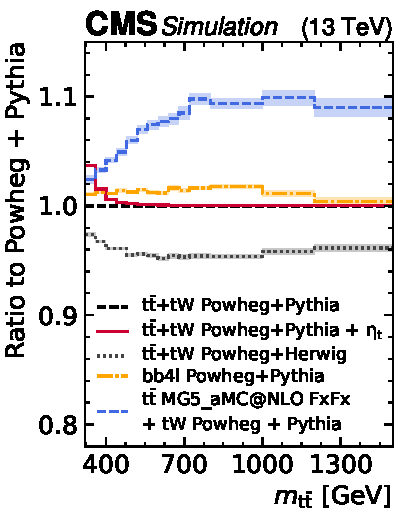
\includegraphics[width=0.32\textwidth]{figures/ah/altbgs/generators_mtt_cms.pdf}
    \hfill
    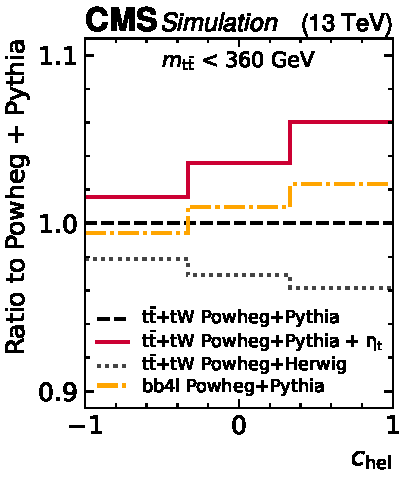
\includegraphics[width=0.32\textwidth]{figures/ah/altbgs/generators_chel_lowmtt_cms.pdf}
    \hfill
    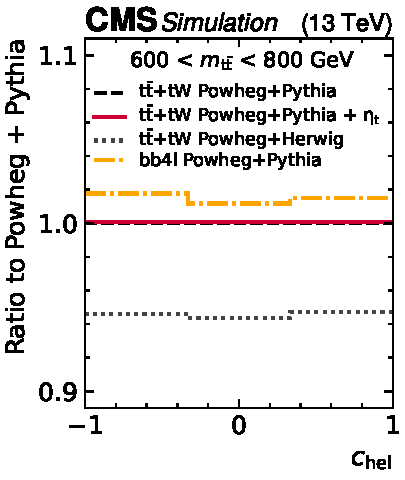
\includegraphics[width=0.32\textwidth]{figures/ah/altbgs/generators_chel_highmtt_cms.pdf}
    \caption{
        \textbf{Comparison between MC generators for \tttWsum.} The ratio of the predictions between \powheg \hvq \ttbar matched to \herwig and to \pythia as well as between \bbfourl and \tttWsum matched to \pythia for the inclusive reconstructed \mtt distribution (left) and the reconstructed \chel distribution, restricted to $\mtt < \SI{360}{\GeV}$ (center) and to $600 < \mtt < \SI{800}{\GeV}$. The effect of the \etat signal is also shown for comparison. \textit{Figure taken from \citere{CMS:TOP-24-007}.}
    }
    \label{fig:ah:herwigbb4l}
\end{figure}

\Cref{fig:ah:herwigbb4l} shows the ratios of the predictions from \herwig and \pythia for the reconstructed \mtt distribution, as well as for the \chel distribution close to the \ttbar threshold (i.e. where the \etat signal is located) and in the \ttbar continuum. Besides a significantly lower \ttbar acceptance, \herwig predicts an increase of events at the \ttbar threshold similar to \etat.
This appears concerning at first glance since, should the data follow the prediction from \herwig instead of \pythia, this enhancement could be confused with an \etat signal if \pythia is used as the baseline prediction.
However, as seen in \cref{fig:ah:herwigbb4l} in the center, \herwig at the same predicts a flatter slope in \chel than \pythia at the \ttbar threshold, equivalent to a dilution of \ttbar spin correlations\footnote{This effect was also seen in the context of \citere{ATLAS:2023fsd}.}. This is in contrast to the \etat signal, in which the \ttbar spins are maximally anti-correlated. The inclusion of the spin correlation variable \chel in the analysis thus makes it possible to separate the differences between \powheg and \herwig with respect to \etat.

The second alternative generator is \bbfourl matched to \pythia, as studied extensively in \cref{ch:bb4l}. Here, particularly the off-shell effects included in \bbfourl might be of interest for the extraction of \etat since the latter is located below the \ttbar threshold. The setup denoted as ``\bbfourl v2'' in \cref{sec:bb4l:bb4l}, corresponding to \citere{Jezo:2023rht}, is used, and compared to the sum of the \powheg \hvq \ttbar and tW predictions for consistency.

A caveat here is presented by the corrections to NNLO QCD and NLO EW as described in \cref{sec:ah:ttbarweights}. These are derived from fixed-order corrections assuming stable top quarks, and are not available for the full \bbllnunu final state. To still be able to apply them to \bbfourl predictions, the \bbfourl sample is split into a \ttbar and a tW part in an ad-hoc way by using the matrix element history projectors implemented in \bbfourl~v2~\cite{Jezo:2023rht}. The corrections are then applied to the \ttbar part only, in the same manner as to \powheg \hvq.

%\begin{figure}[!t]
%    \centering
%    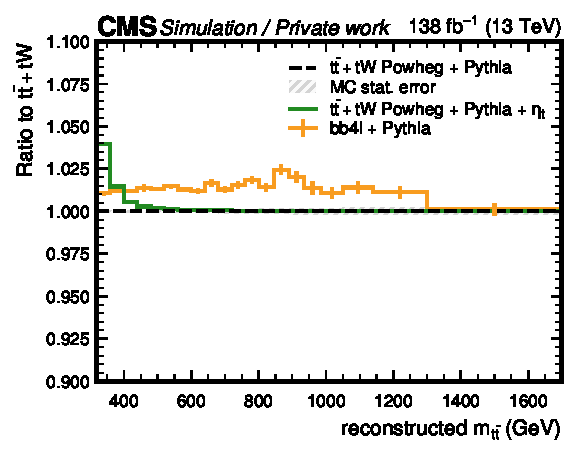
\includegraphics[width=0.49\textwidth]{figures/ah/altbgs/hvqvsbb4l_mtt.pdf}
%    \hfill
%    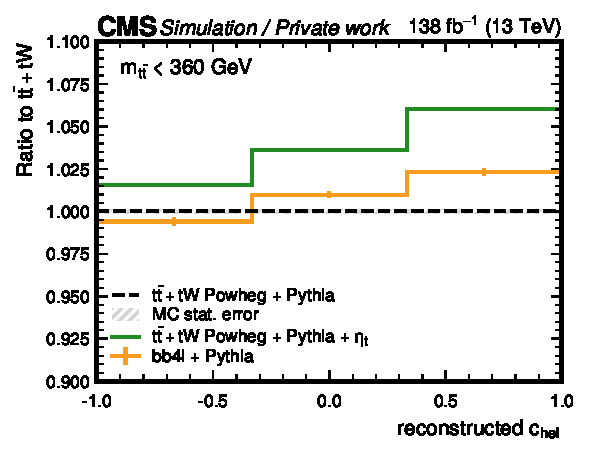
\includegraphics[width=0.49\textwidth]{figures/ah/altbgs/hvqvsbb4l_chel_lowmtt.pdf}
%    \caption{
%        \textbf{Comparison of \powheg \tttWsum and \bbfourl.} The ratio of the predictions of the sum of \powheg \hvq \ttbar and tW to \bbfourl (all matched to \pythia) for the inclusive reconstructed \mtt distribution (left) and the reconstructed \chel distribution, restricted to $\mtt < \SI{360}{\GeV}$ (right). The effect of the \etat signal is also shown for comparison.
%    }
%    \label{fig:ah:bb4l}
%\end{figure}

The ratios of the predictions are also shown in \cref{fig:ah:herwigbb4l}. It can be seen that \bbfourl does not predict major differences in the reconstructed \mtt spectrum even at its lower edge. However, it results in a significantly steeper slope in reconstructed \chel close to the threshold. This increase in slope is of similar magnitude as the effect expected due to \etat. 

The source of this difference is not yet fully understood. \bbfourl contains NLO QCD corrections to the top decay which are not present in \hvq (though they are approximated through the matrix element corrections in \pythia). However, NLO corrections to spin correlations are expected to not only be small, but reduce the spin correlation instead of enhancing it~\cite{Bernreuther:2004jv}. 

It is possible that the effect instead originates in the \tttW interference:
%The tW contribution on its own is expected to have close to flat \chel since one of the leptons is not actually the decay product of a top quark, and the interference between \ttbar and tW is destructive in large parts of the phase space. If the interference in \bbfourl is now larger than in \tttWsum, it could thus reduce the contribution from tW, effectively enhancing the \chel slope. 
For the tW contribution, where one of the leptons is not actually the decay product of a top quark, \ttbar spin correlation is not truly definable. The slope of the reconstructed \chel distribution, obtained under the assumption that the events contain a \ttbar system, will thus be arbitrary with no clear \textit{a priori} expectation, and in general different to the slope in SM \ttbar. The same holds for the \tttW interference. Since \bbfourl now gives a true (though effectively LO) prediction of the \tttW interference instead of the ad-hoc treatment of the DR and DS schemes (cf. \cref{sec:bb4l:others}), it is expected that the magnitude of the interference contribution in \bbfourl will be different. Thus, it is possible that the total \chel slope, arising from the combination of \ttbar, tW, and \tttW interference, will be different as well.
However, since \ttbar and tW are not cleanly separable in \bbfourl, however, this hypothesis is difficult to confirm, and such studies are beyond the scope of this analysis.

%For the purpose of the \etat extraction, the differences to these alternative generator setups are included in the fit as two additional shape-based nuisance parameters (one for \pythia compared to \herwig, and one for \tttWsum compared to \bbfourl). In both cases, the \powheg \hvq + \pythia prediction is considered the nominal, and the alternate prediction is considered the $+1\sigma$ template. The $-1\sigma$ template is constructed by symmetrizing the relative difference around the nominal, and intermediate values are obtained by interpolation as usual. \todo{where are the NPs used and where not}

A third alternative prediction is provided by \ttbar+jets production simulated with \amcatnlo, matched to \pythia with the FxFx scheme~\cite{Frederix:2012ps}. While this prediction is formally also NLO-accurate in QCD in the NWA, and thus comparable to \powheg \hvq, it has been observed in past measurements that \amcatnlo does not agree as well with data as \powheg for \ttbar production. As a result, \amcatnlo is given less focus compared to the other two predictions in this work.

In this work, \powheg \hvq + \pythia is considered for the nominal background prediction in all cases. A comparison to \powheg \hvq + \herwig, \amcatnlo + \pythia, and \bbfourl + \pythia is shown in \cref{sec:ah:checks} in the context of measuring the \etat cross section. Furthermore, the effect of including the differences to \powheg \hvq + \herwig and \bbfourl + \pythia as two additional shape-based nuisance parameters in the fit is similarly given in \cref{sec:ah:checks}. Note that in \citere{CMS:TOP-24-007}, these nuisance parameters were considered as part of the main result in order to be conservative with respect to the total uncertainty.

\section{Pre-fit distributions}
\label{sec:ah:prefit}

\begin{figure}[!hp]
    \centering
    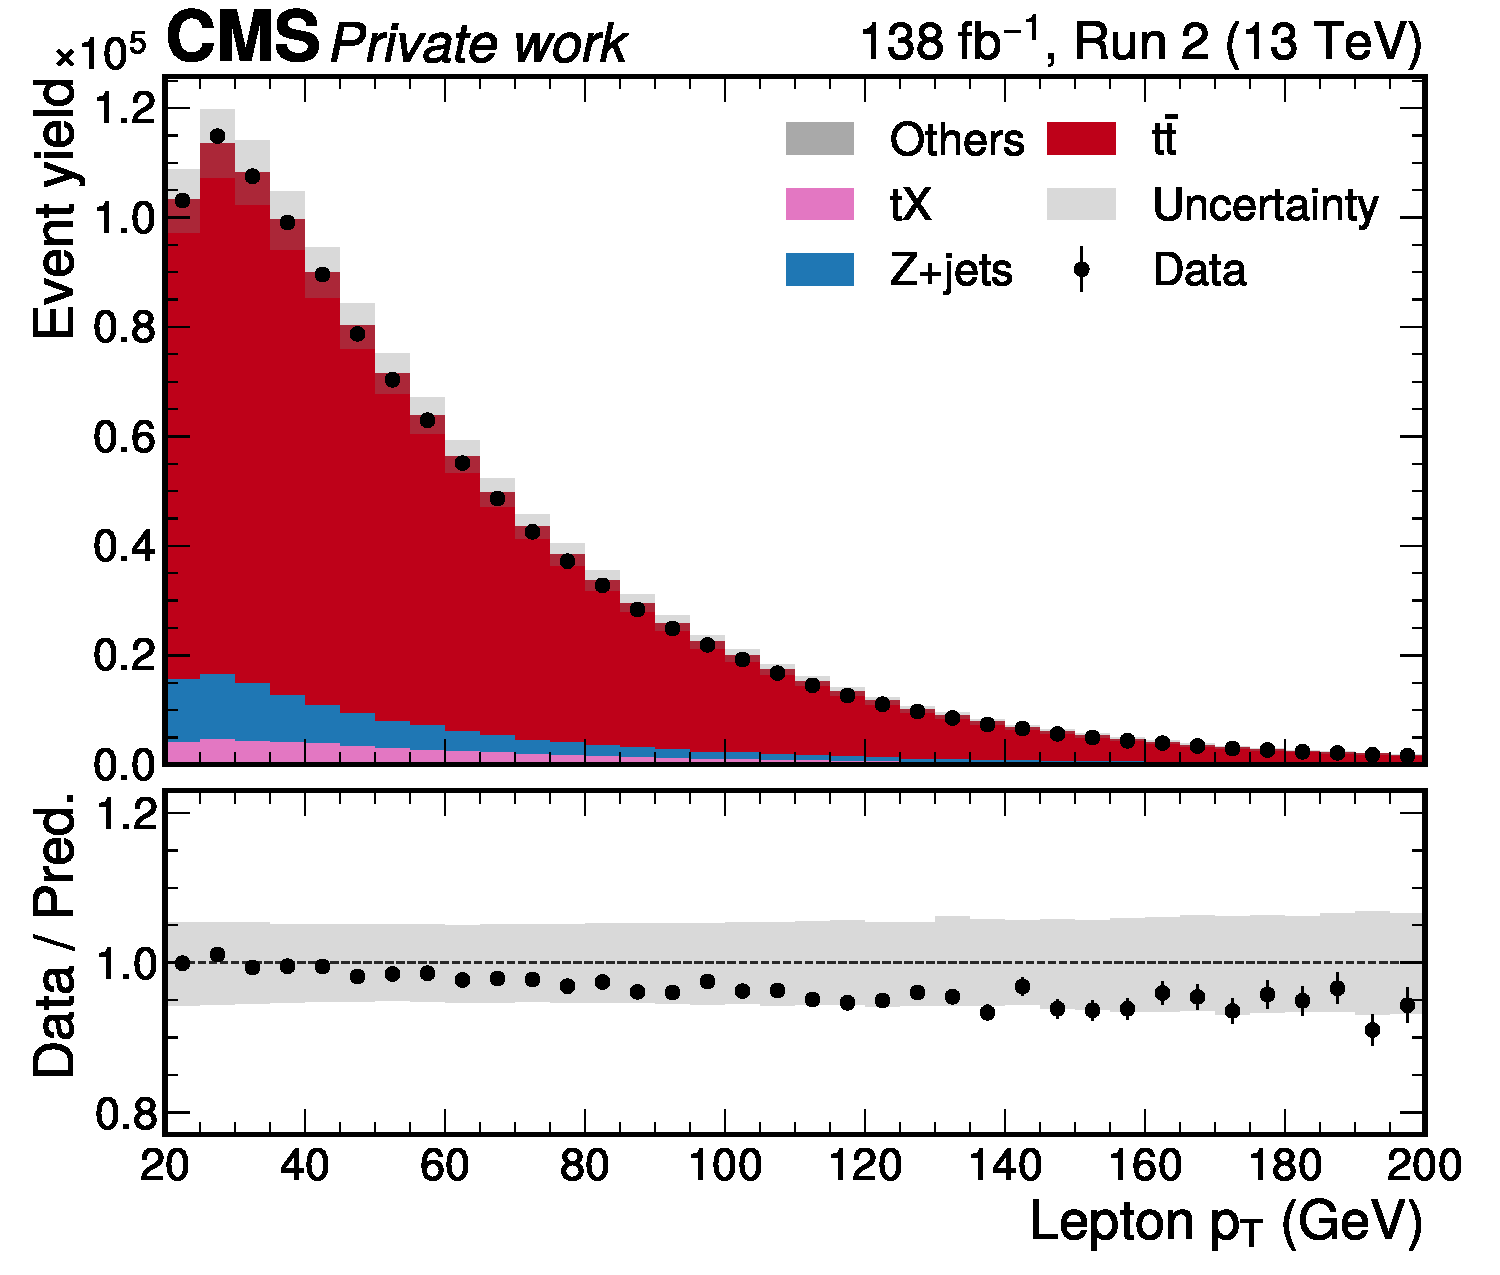
\includegraphics[width=0.49\textwidth]{figures/ah/controlplots/ReqMET/sf/lep_pt_ReqMET_sf.pdf}
    \hfill
    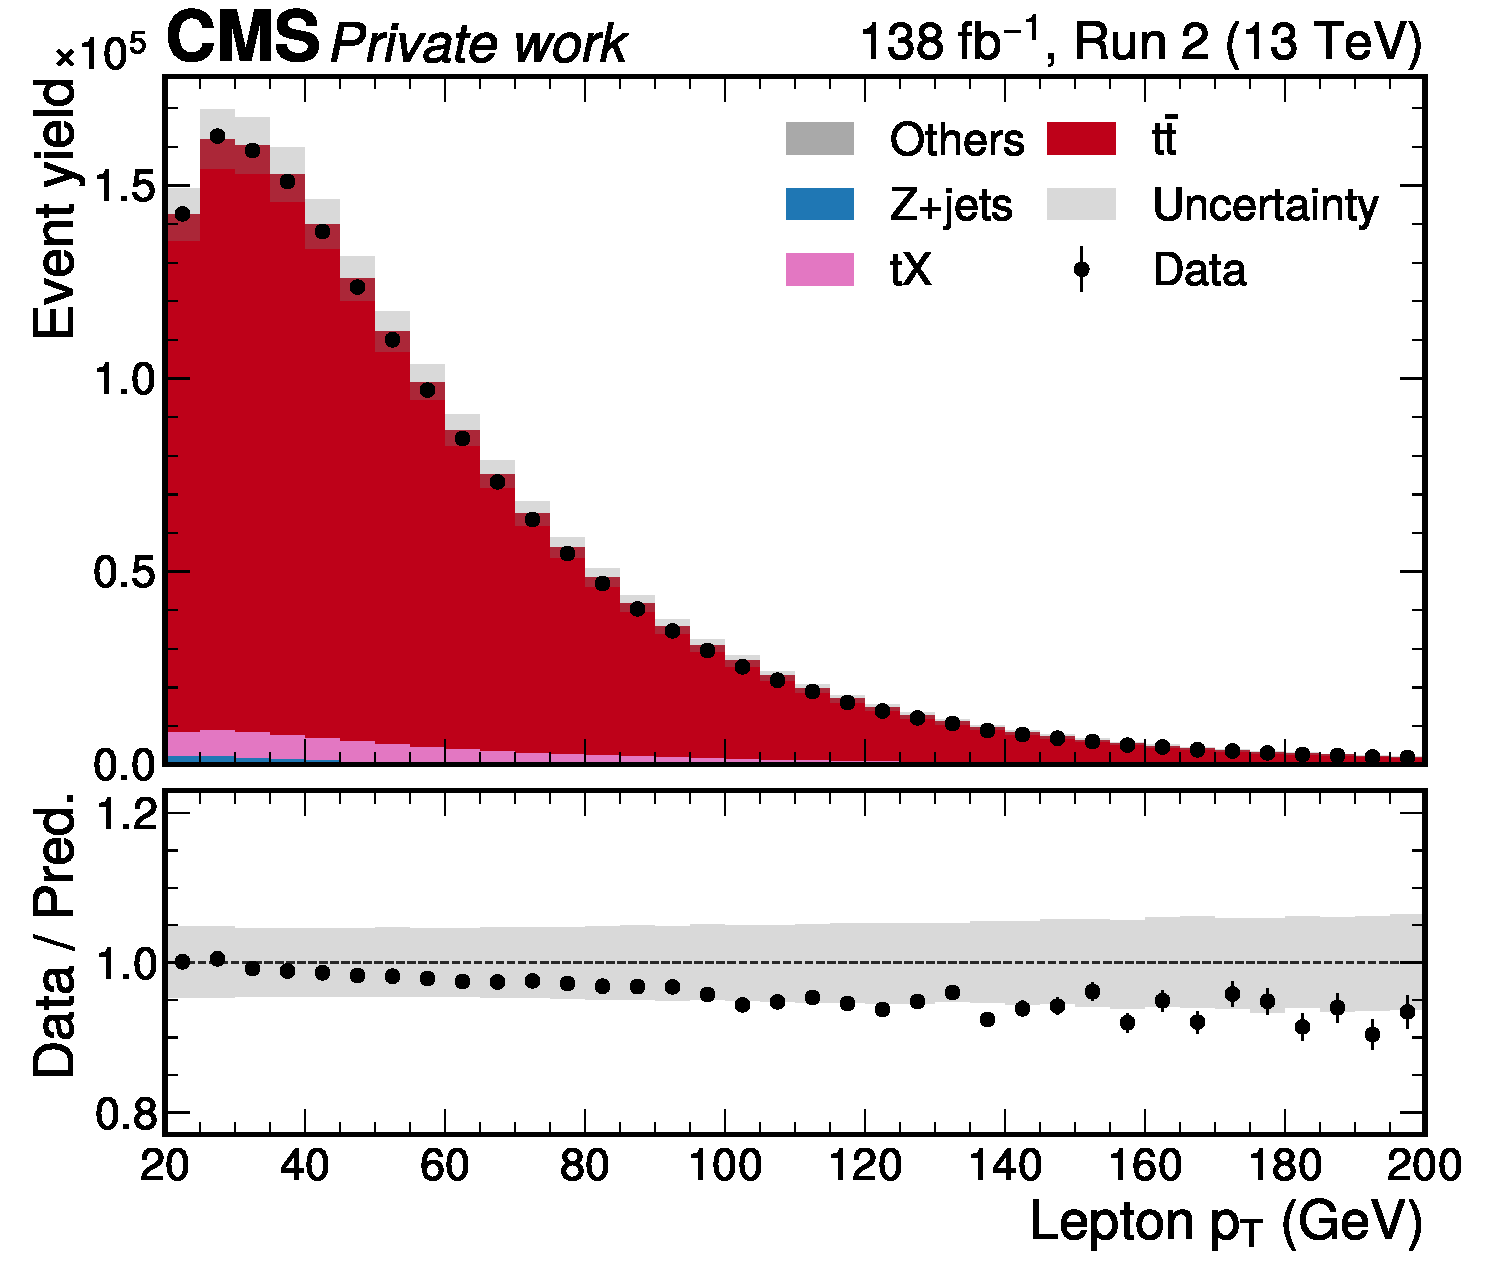
\includegraphics[width=0.49\textwidth]{figures/ah/controlplots/ReqMET/em/lep_pt_ReqMET_em.pdf}
    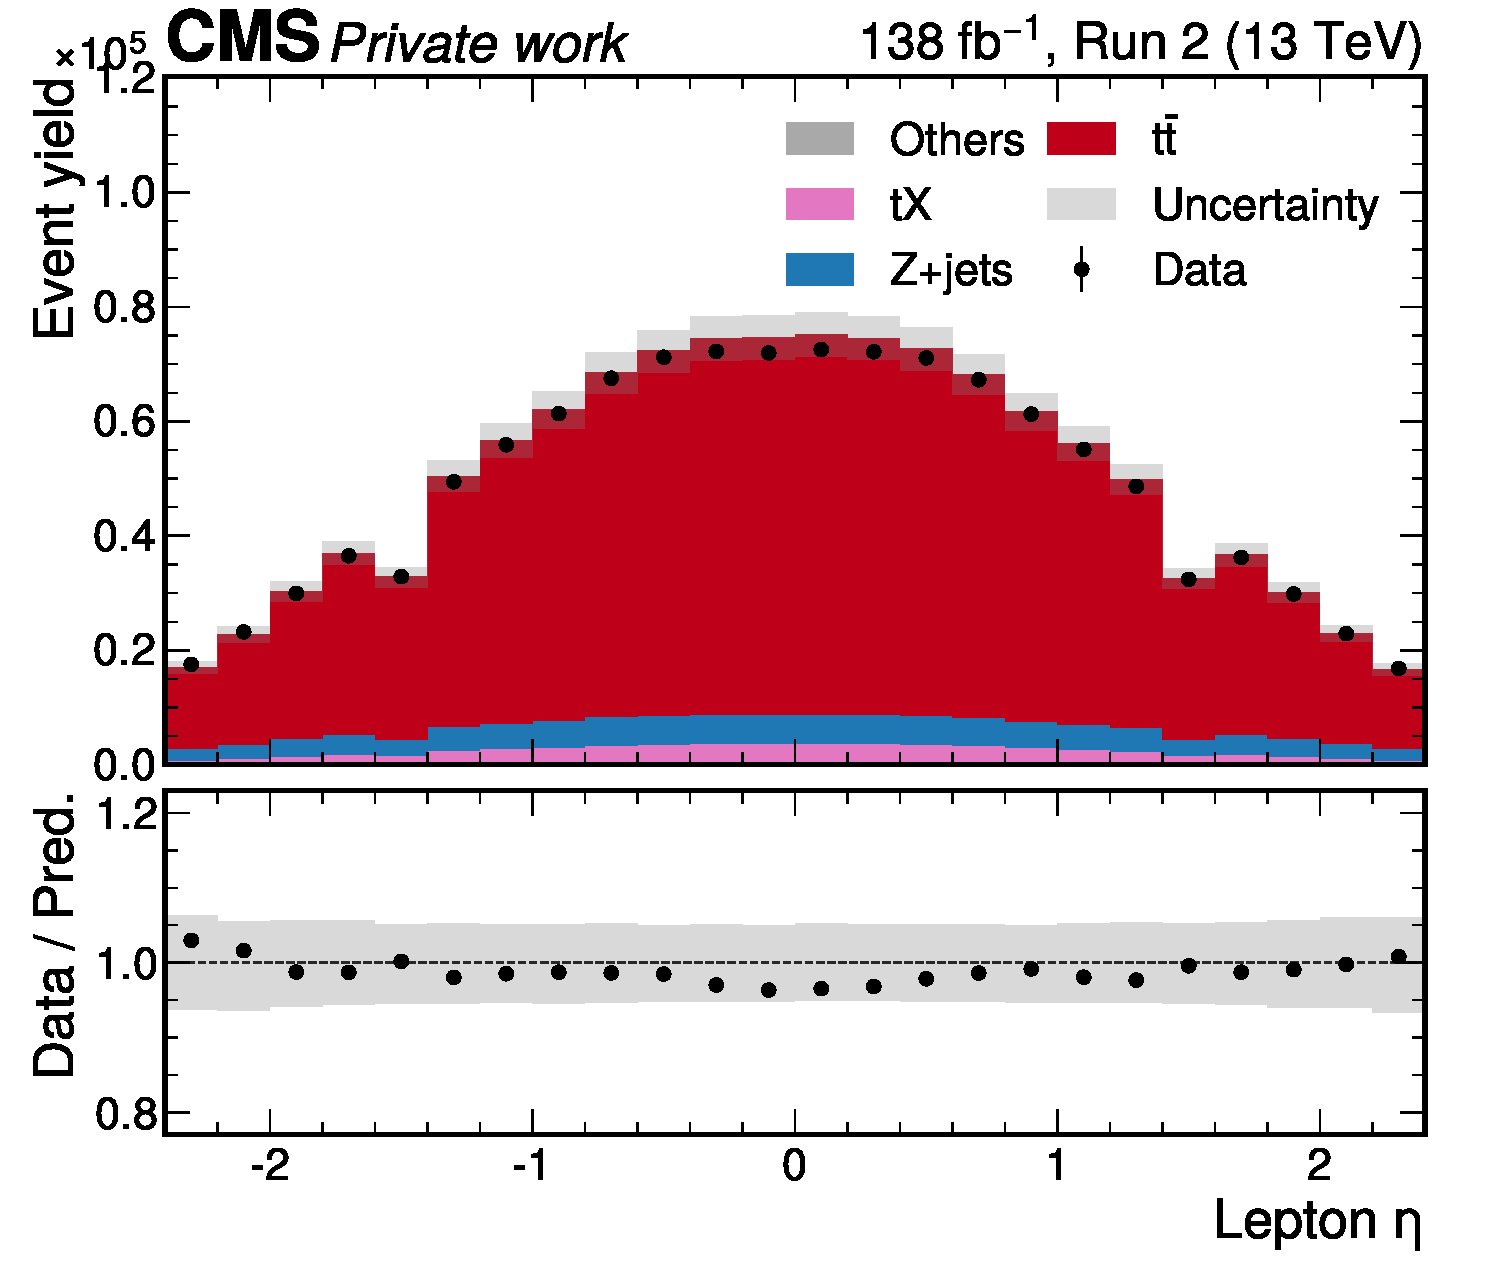
\includegraphics[width=0.49\textwidth]{figures/ah/controlplots/ReqMET/sf/lep_eta_ReqMET_sf.pdf}
    \hfill
    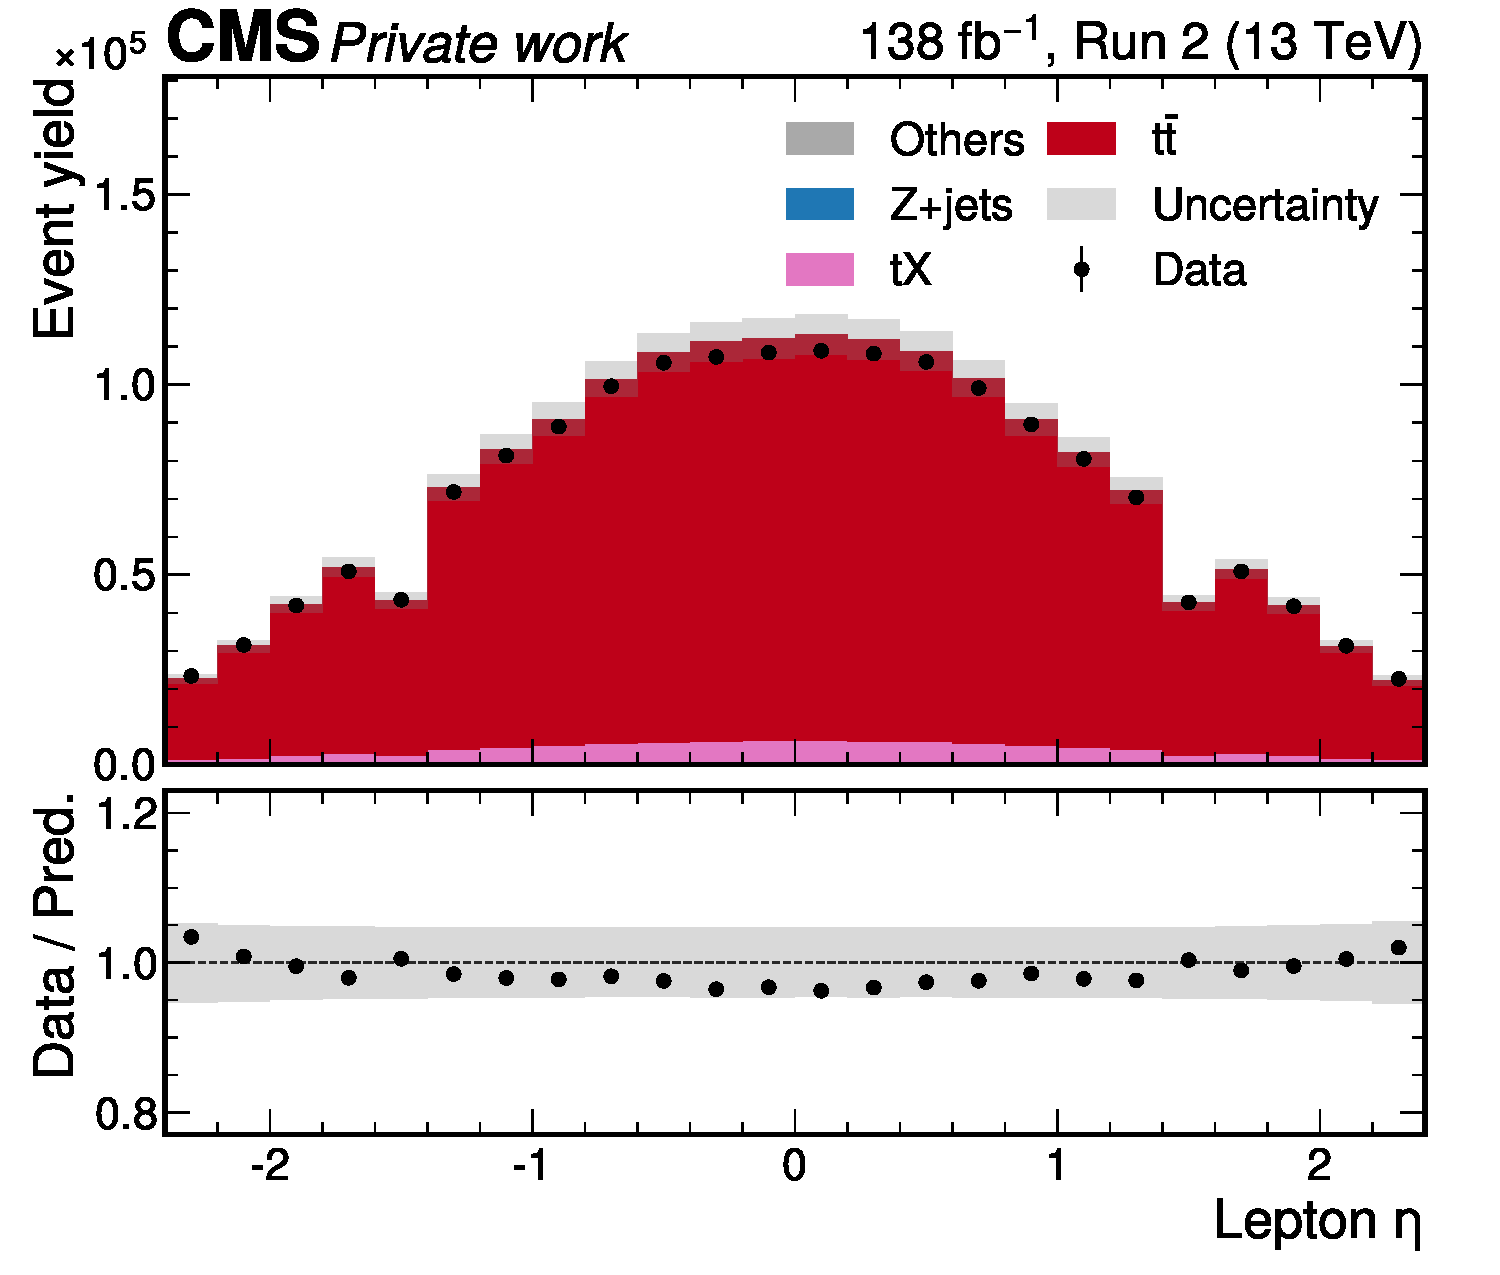
\includegraphics[width=0.49\textwidth]{figures/ah/controlplots/ReqMET/em/lep_eta_ReqMET_em.pdf}
    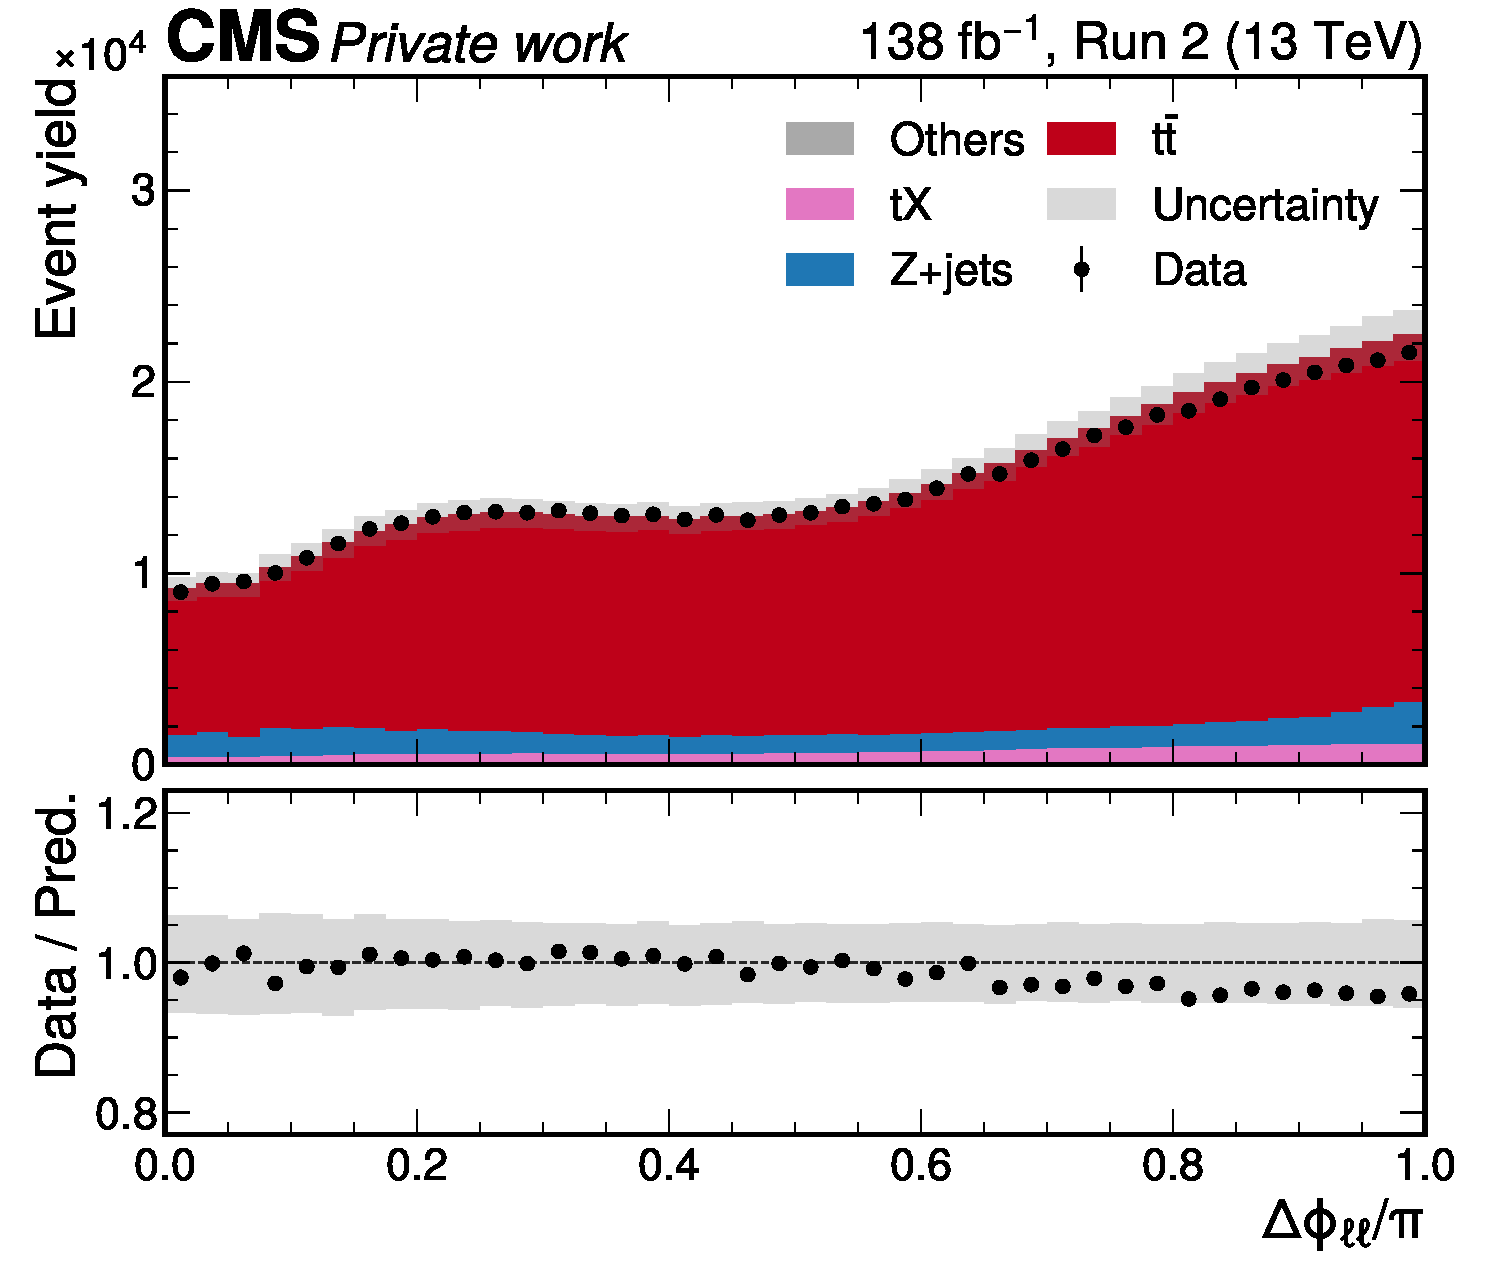
\includegraphics[width=0.49\textwidth]{figures/ah/controlplots/ReqMET/sf/lep_deltaphi_ReqMET_sf.pdf}
    \hfill
    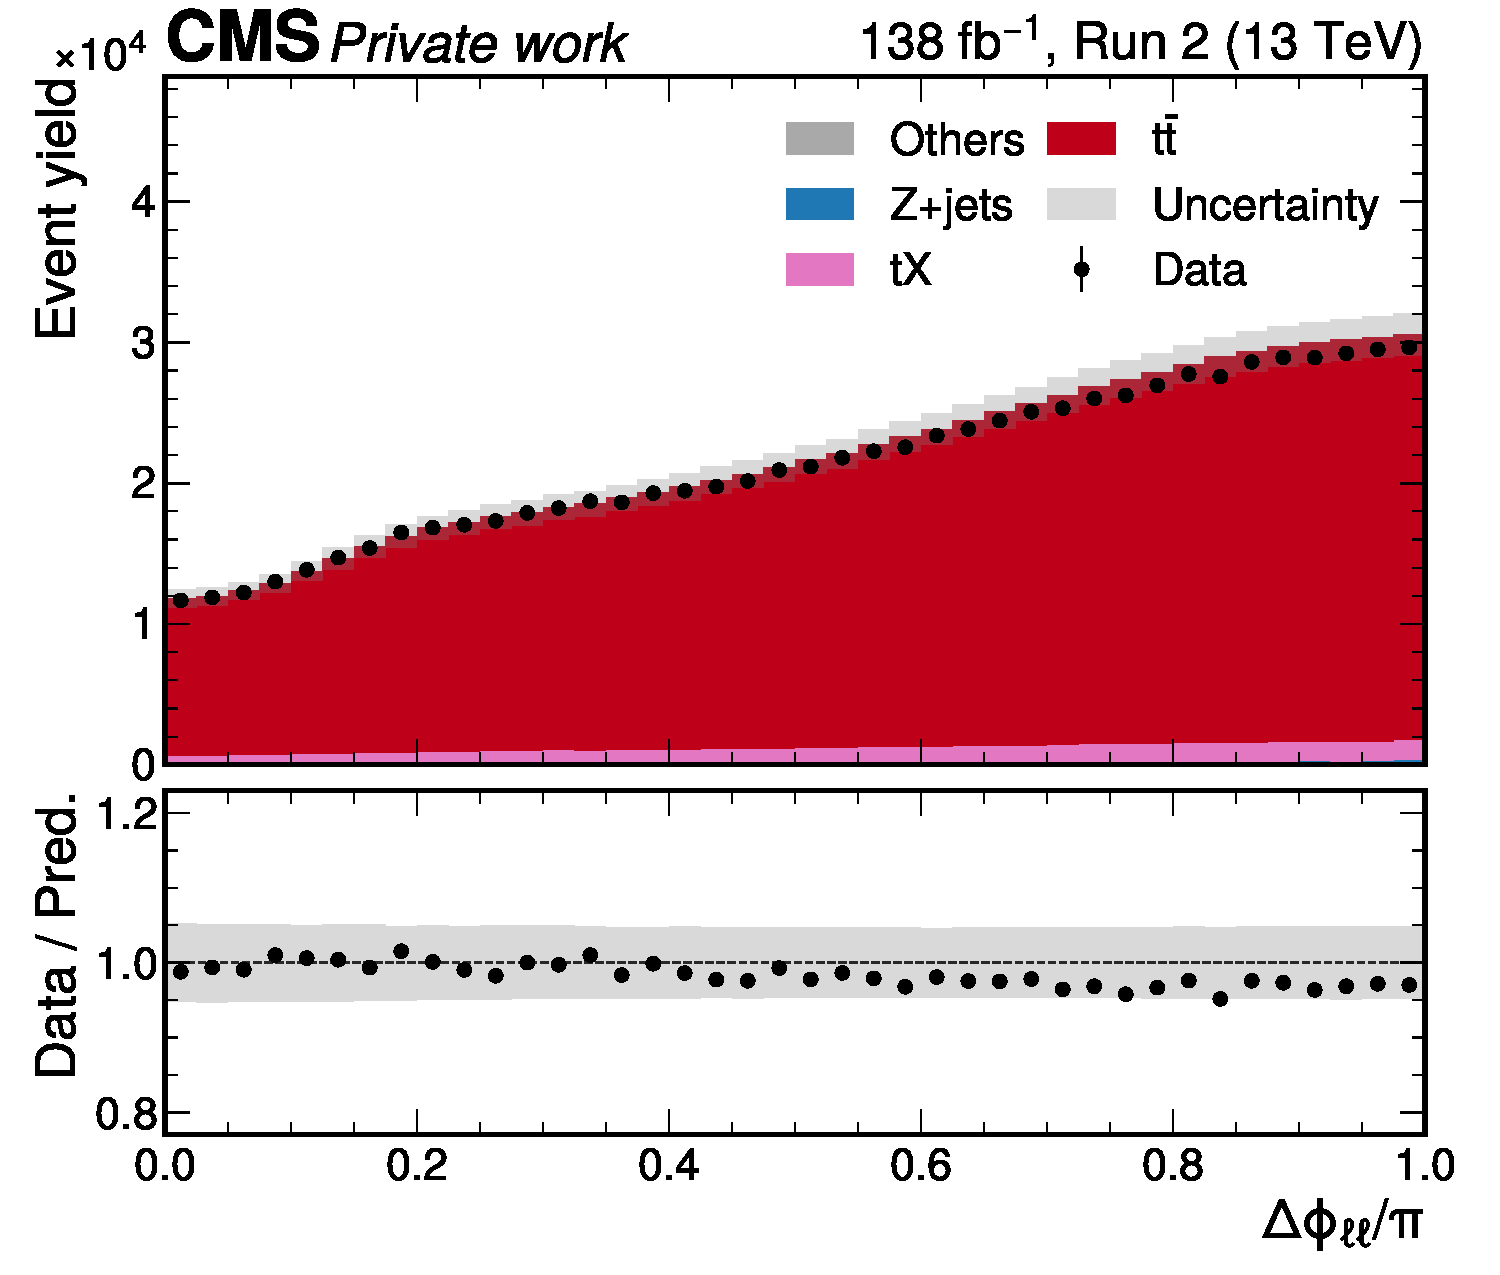
\includegraphics[width=0.49\textwidth]{figures/ah/controlplots/ReqMET/em/lep_deltaphi_ReqMET_em.pdf}
    \caption{
        \textbf{Control distributions.} Shown are the distributions of \pt of both leptons (top), $\eta$ of both leptons (center), and the azimuthal angle \dphill between the leptons (bottom) in the \ee/\mumu (left) and \emu channels (right). All figures show both data (black dots) and different simulated background processes (colored bars), as well as the total systematic uncertainty (gray band). 
    }
    \label{fig:ah:control1}
\end{figure}

\begin{figure}[!hp]
    \centering
    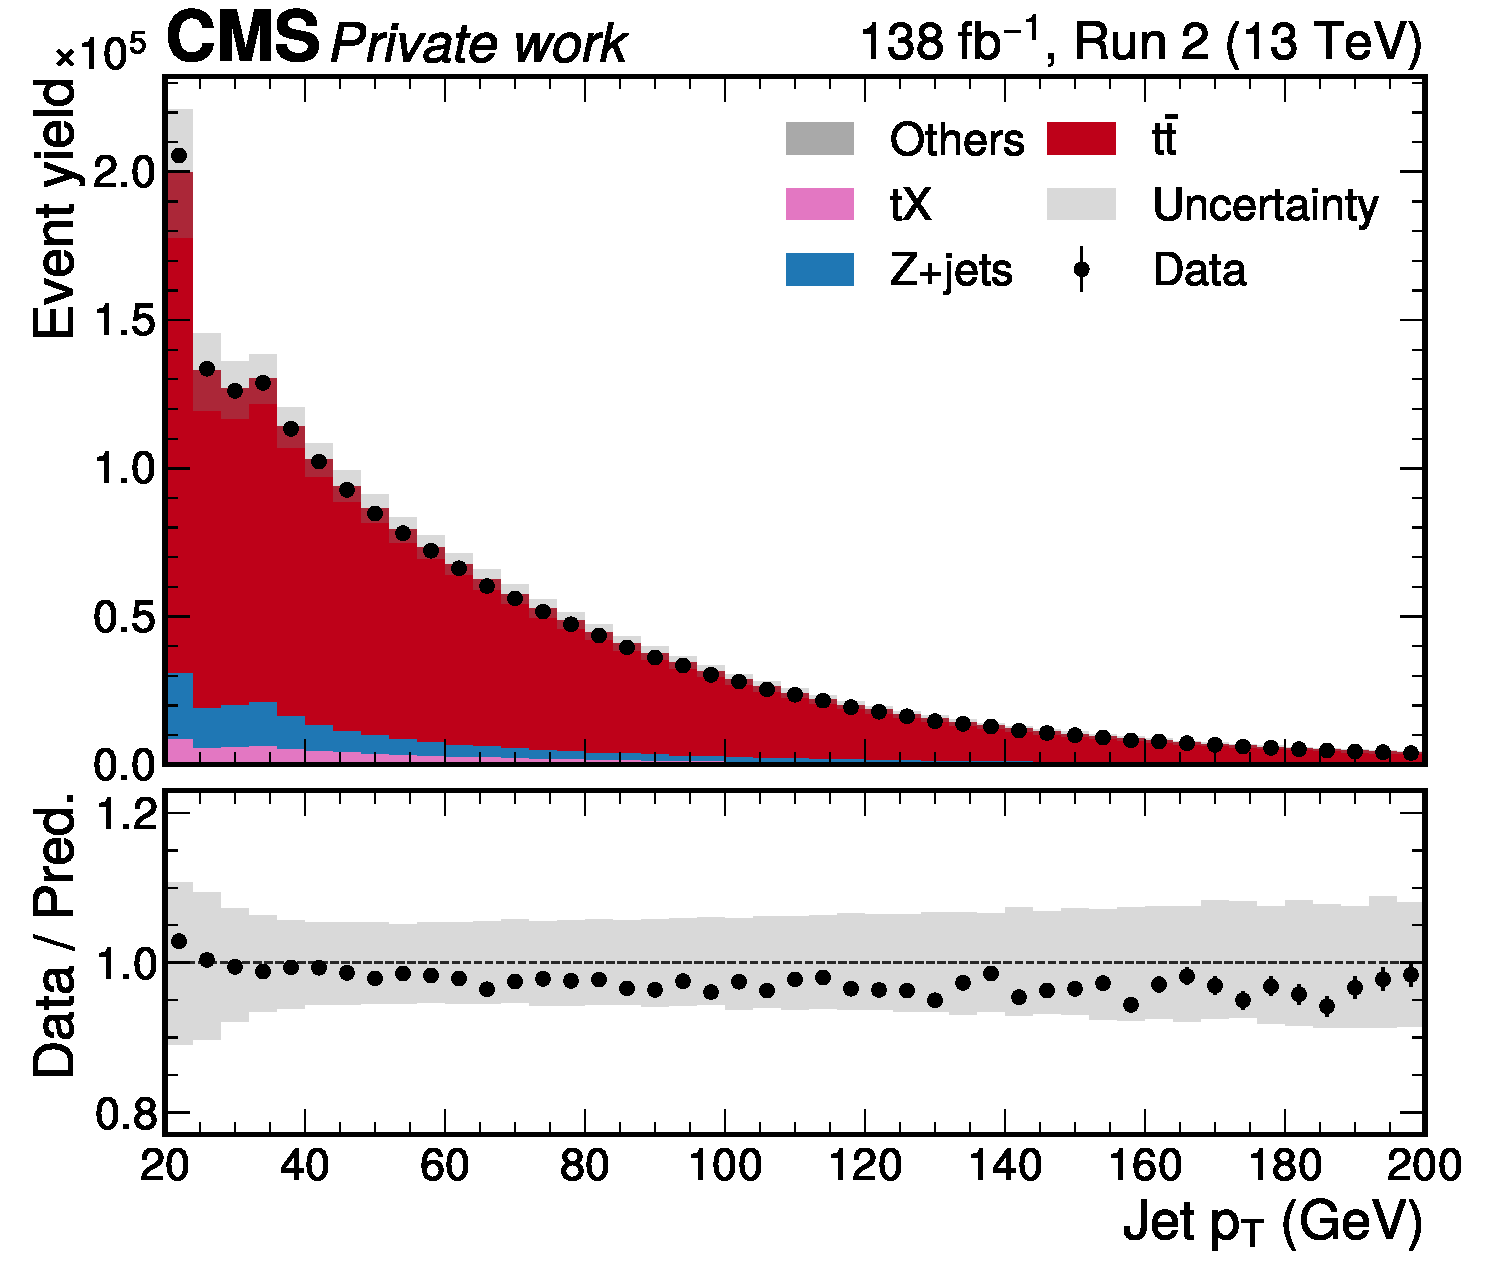
\includegraphics[width=0.49\textwidth]{figures/ah/controlplots/ReqMET/sf/jet_pt_ReqMET_sf.pdf}
    \hfill
    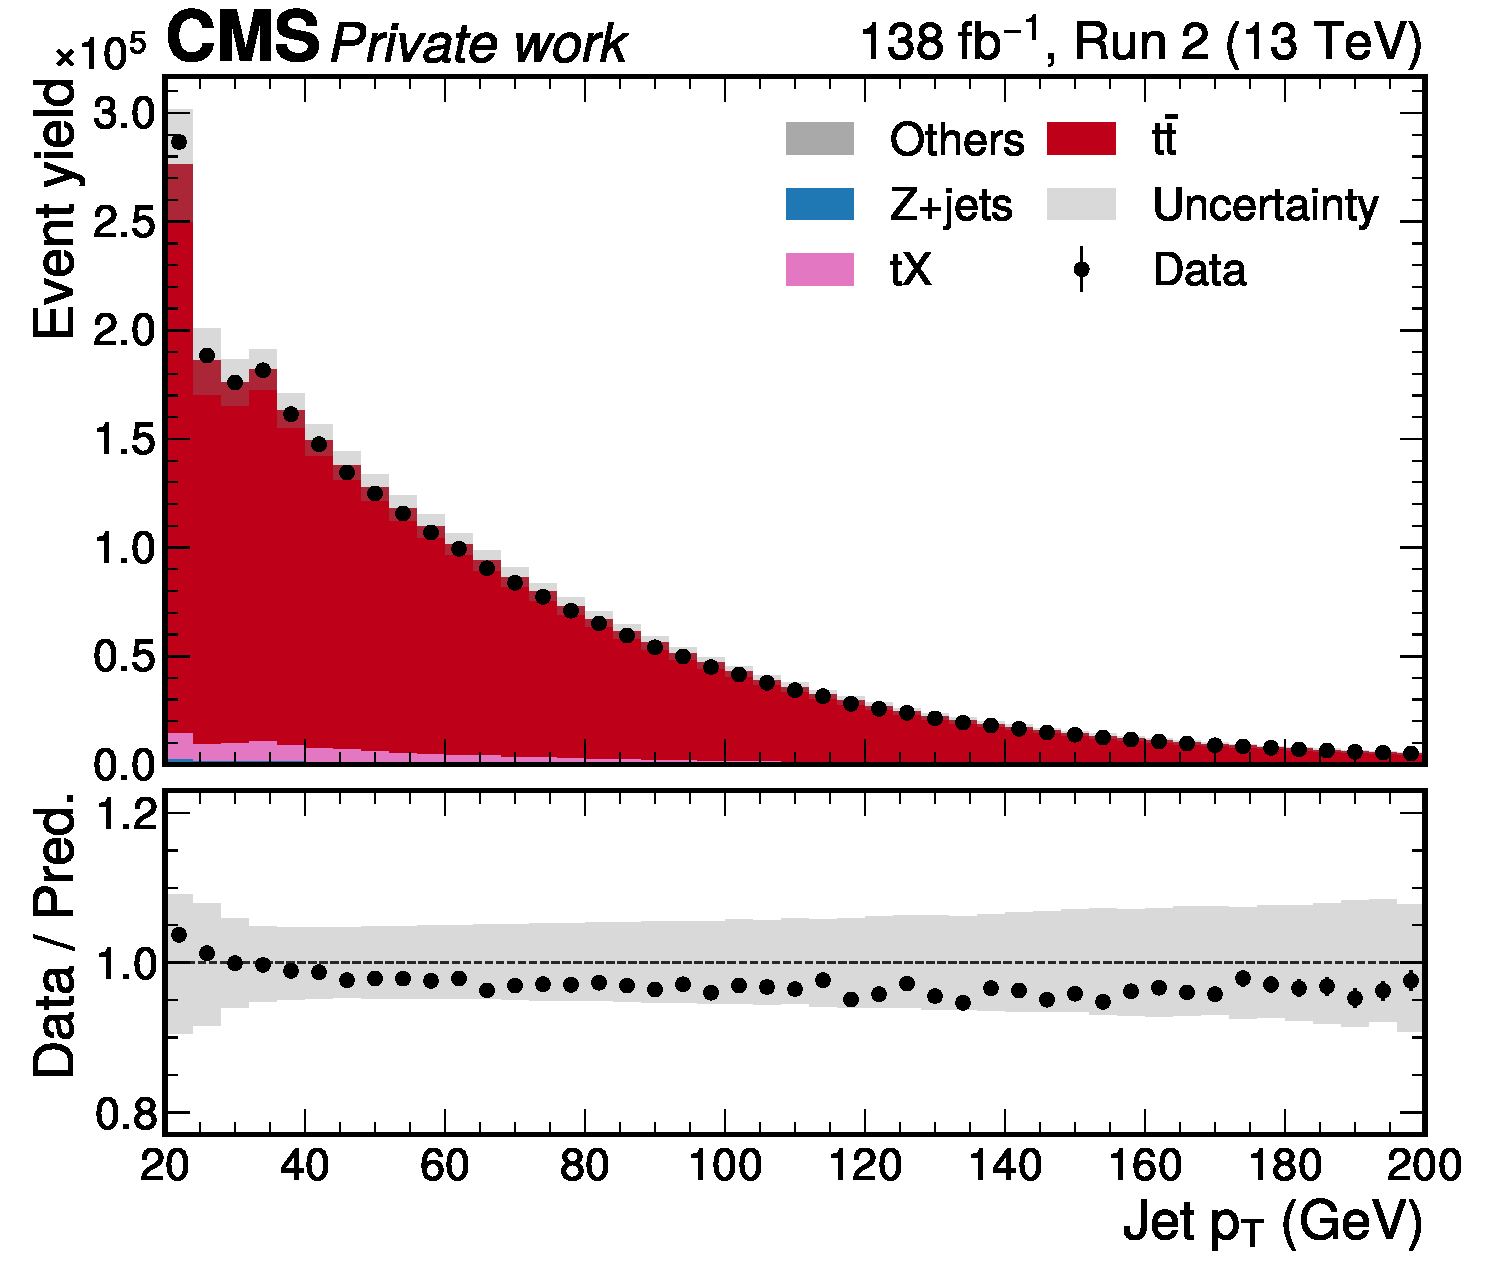
\includegraphics[width=0.49\textwidth]{figures/ah/controlplots/ReqMET/em/jet_pt_ReqMET_em.pdf}
    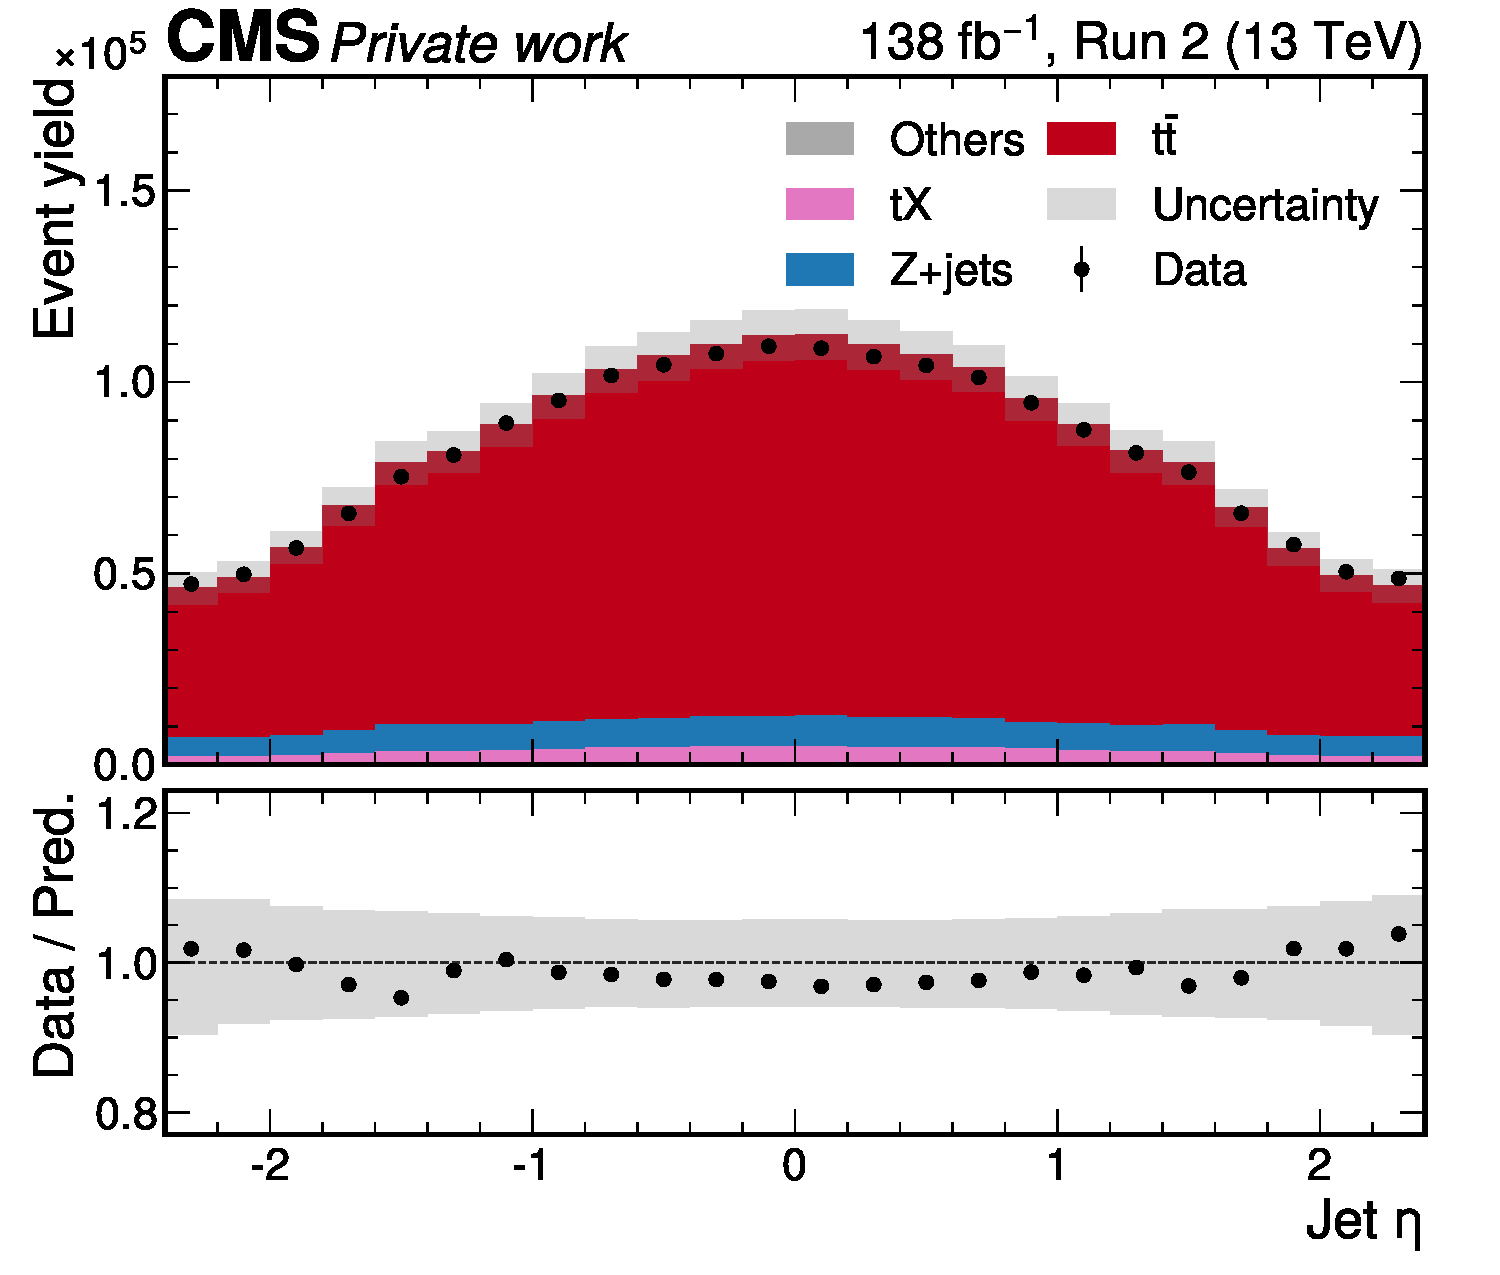
\includegraphics[width=0.49\textwidth]{figures/ah/controlplots/ReqMET/sf/jet_eta_ReqMET_sf.pdf}
    \hfill
    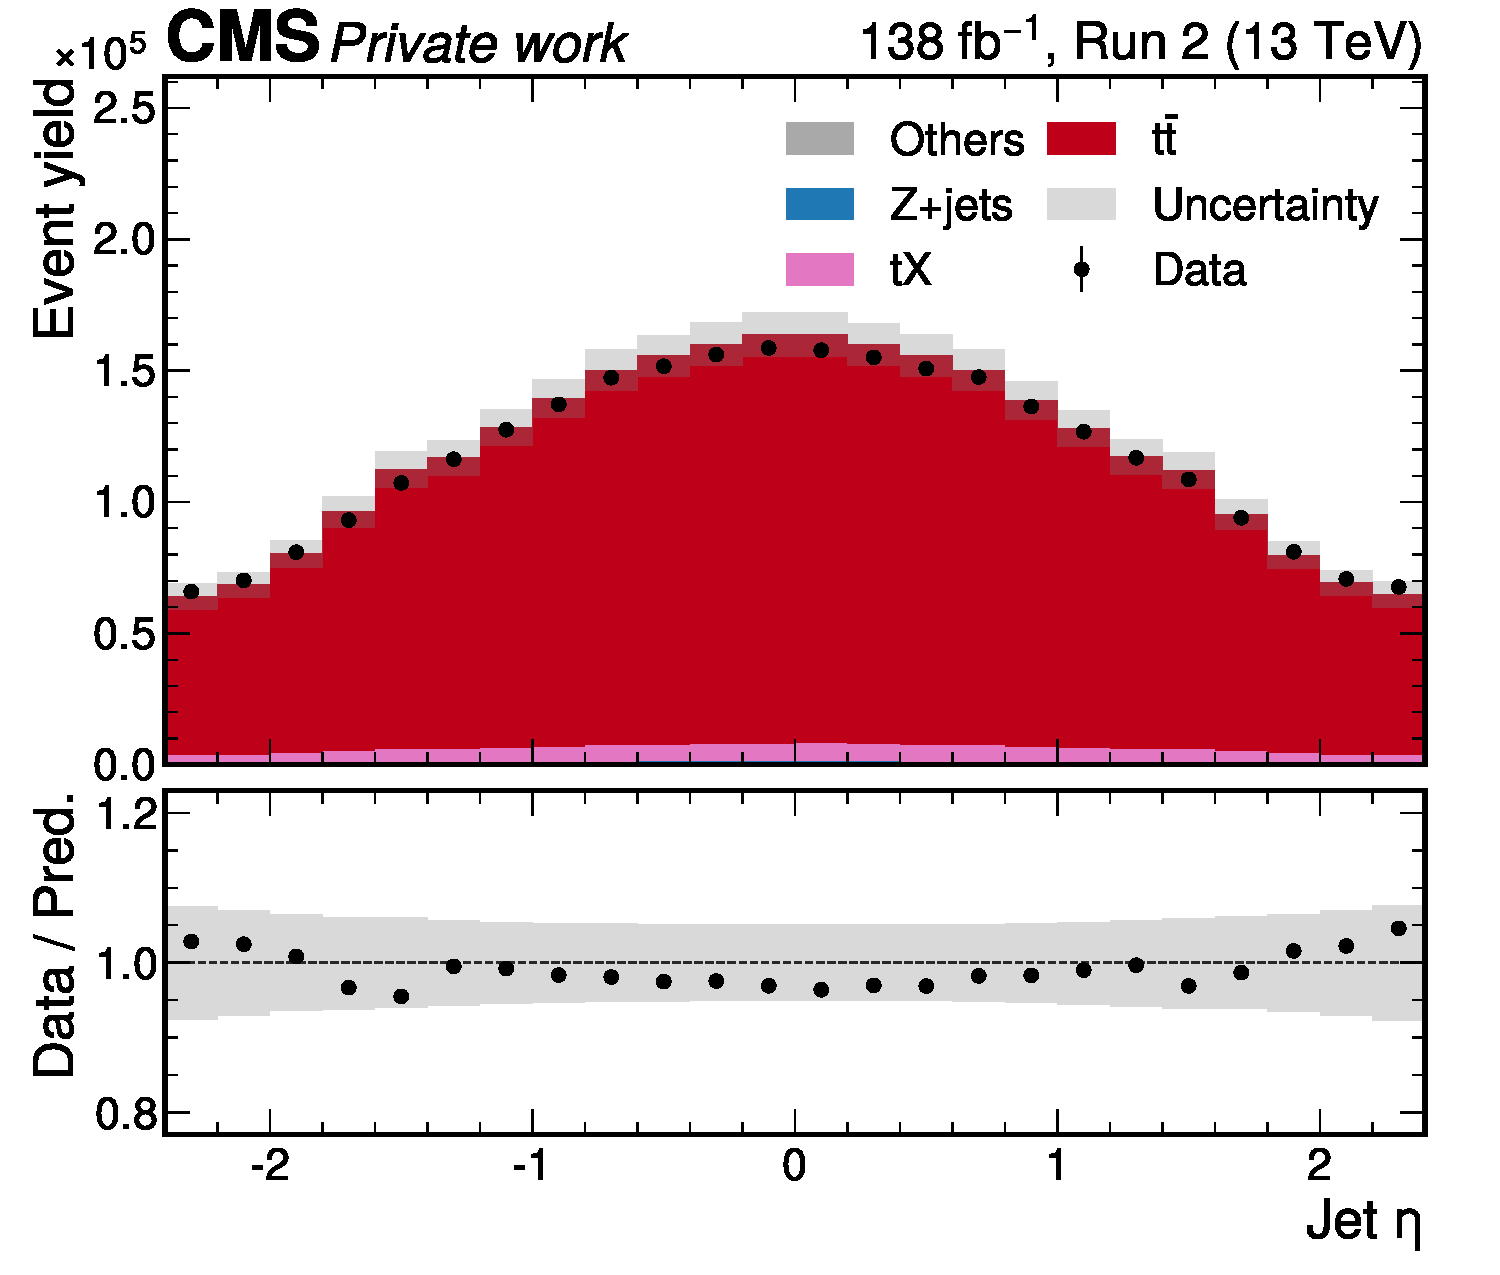
\includegraphics[width=0.49\textwidth]{figures/ah/controlplots/ReqMET/em/jet_eta_ReqMET_em.pdf}
    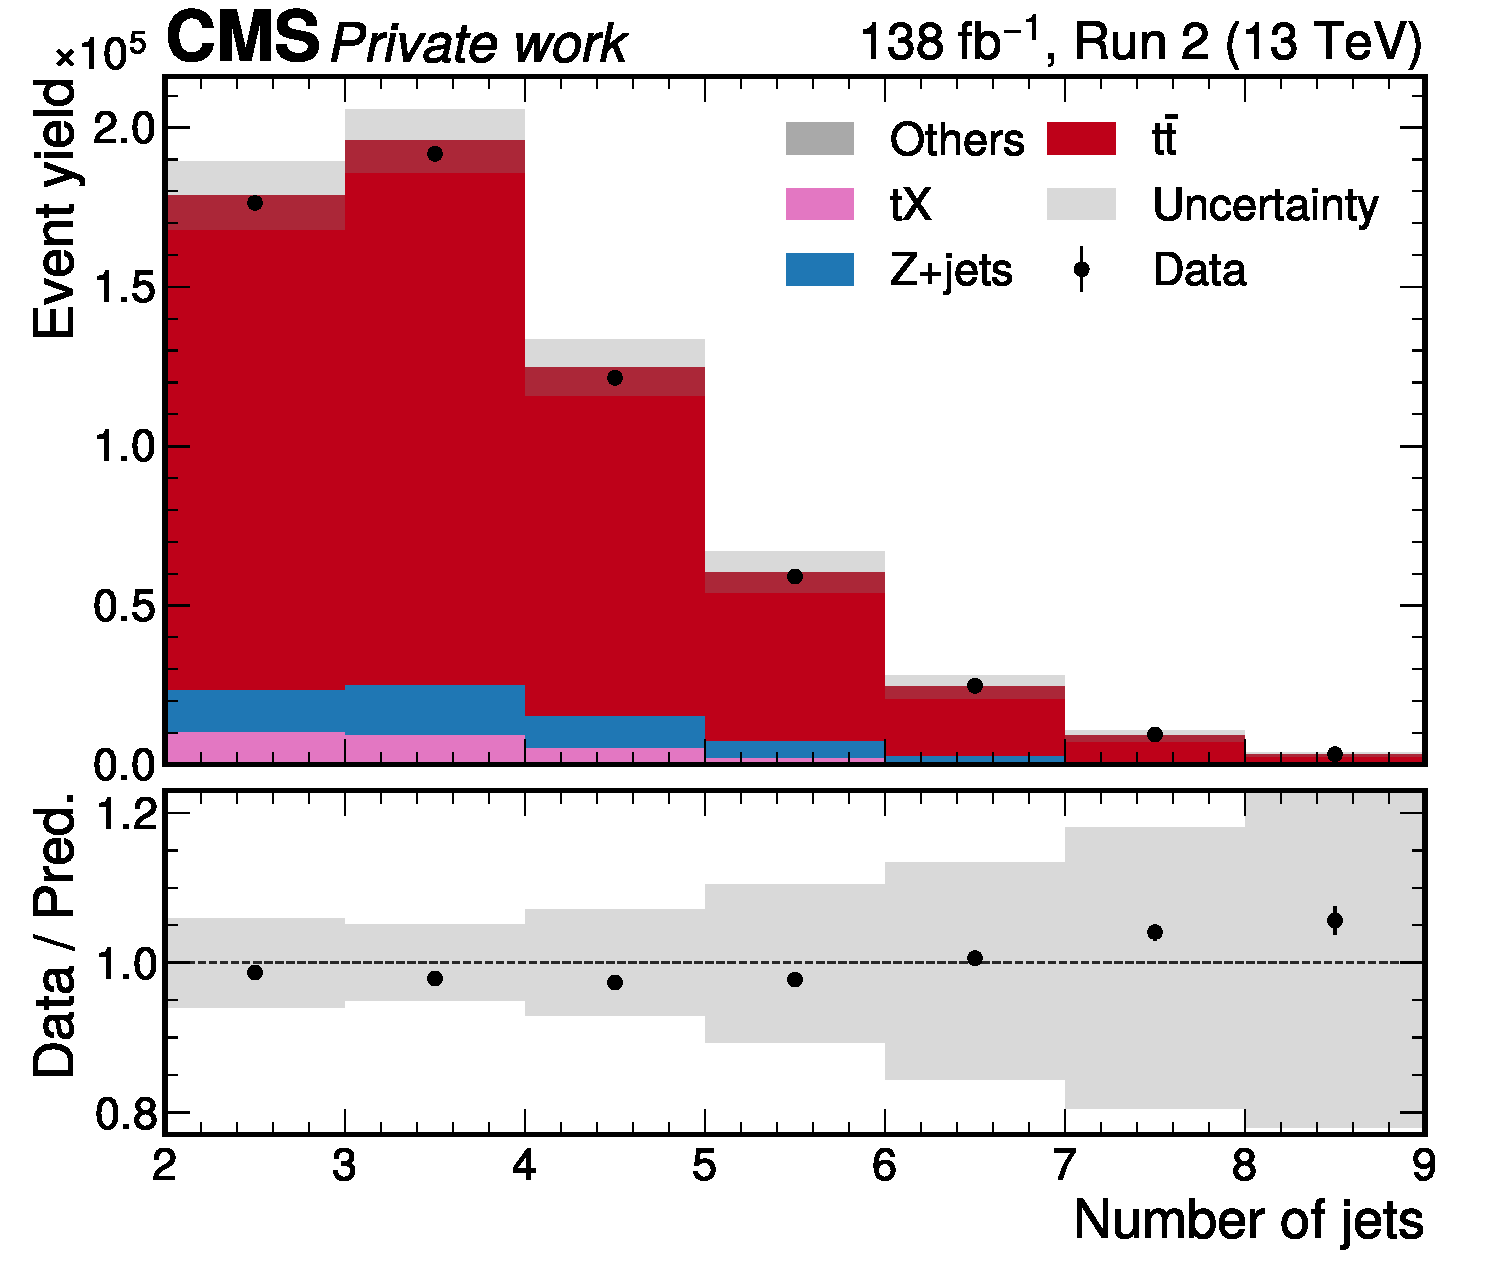
\includegraphics[width=0.49\textwidth]{figures/ah/controlplots/ReqMET/sf/njet_ReqMET_sf.pdf}
    \hfill
    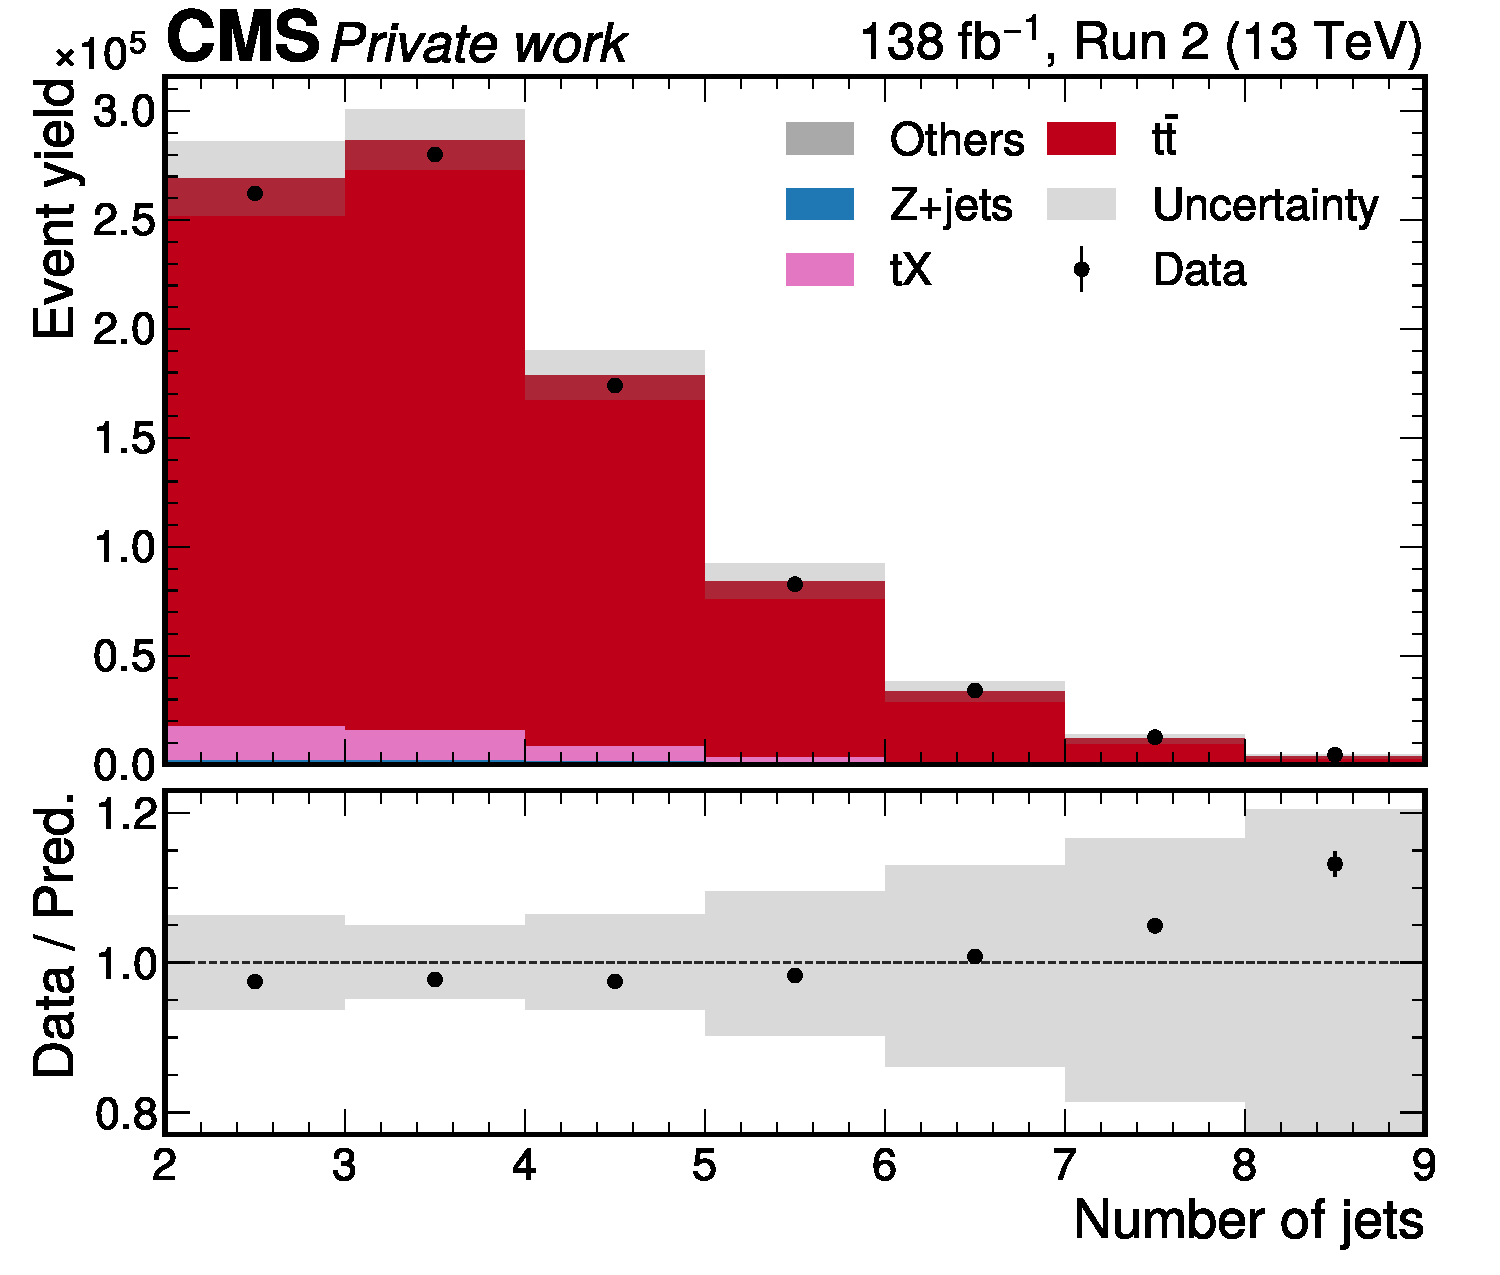
\includegraphics[width=0.49\textwidth]{figures/ah/controlplots/ReqMET/em/njet_ReqMET_em.pdf}
    \caption{
        \textbf{Control distributions.} Shown are the distributions of \pt of all jets (top), $\eta$ of all jets (center), and the number of jets (bottom) in the \ee/\mumu (left) and \emu channels (right). All figures show both data (black dots) and different simulated background processes (colored bars), as well as the total systematic uncertainty (gray band). 
    }
    \label{fig:ah:control2}
\end{figure}

\begin{figure}[!hp]
    \centering
    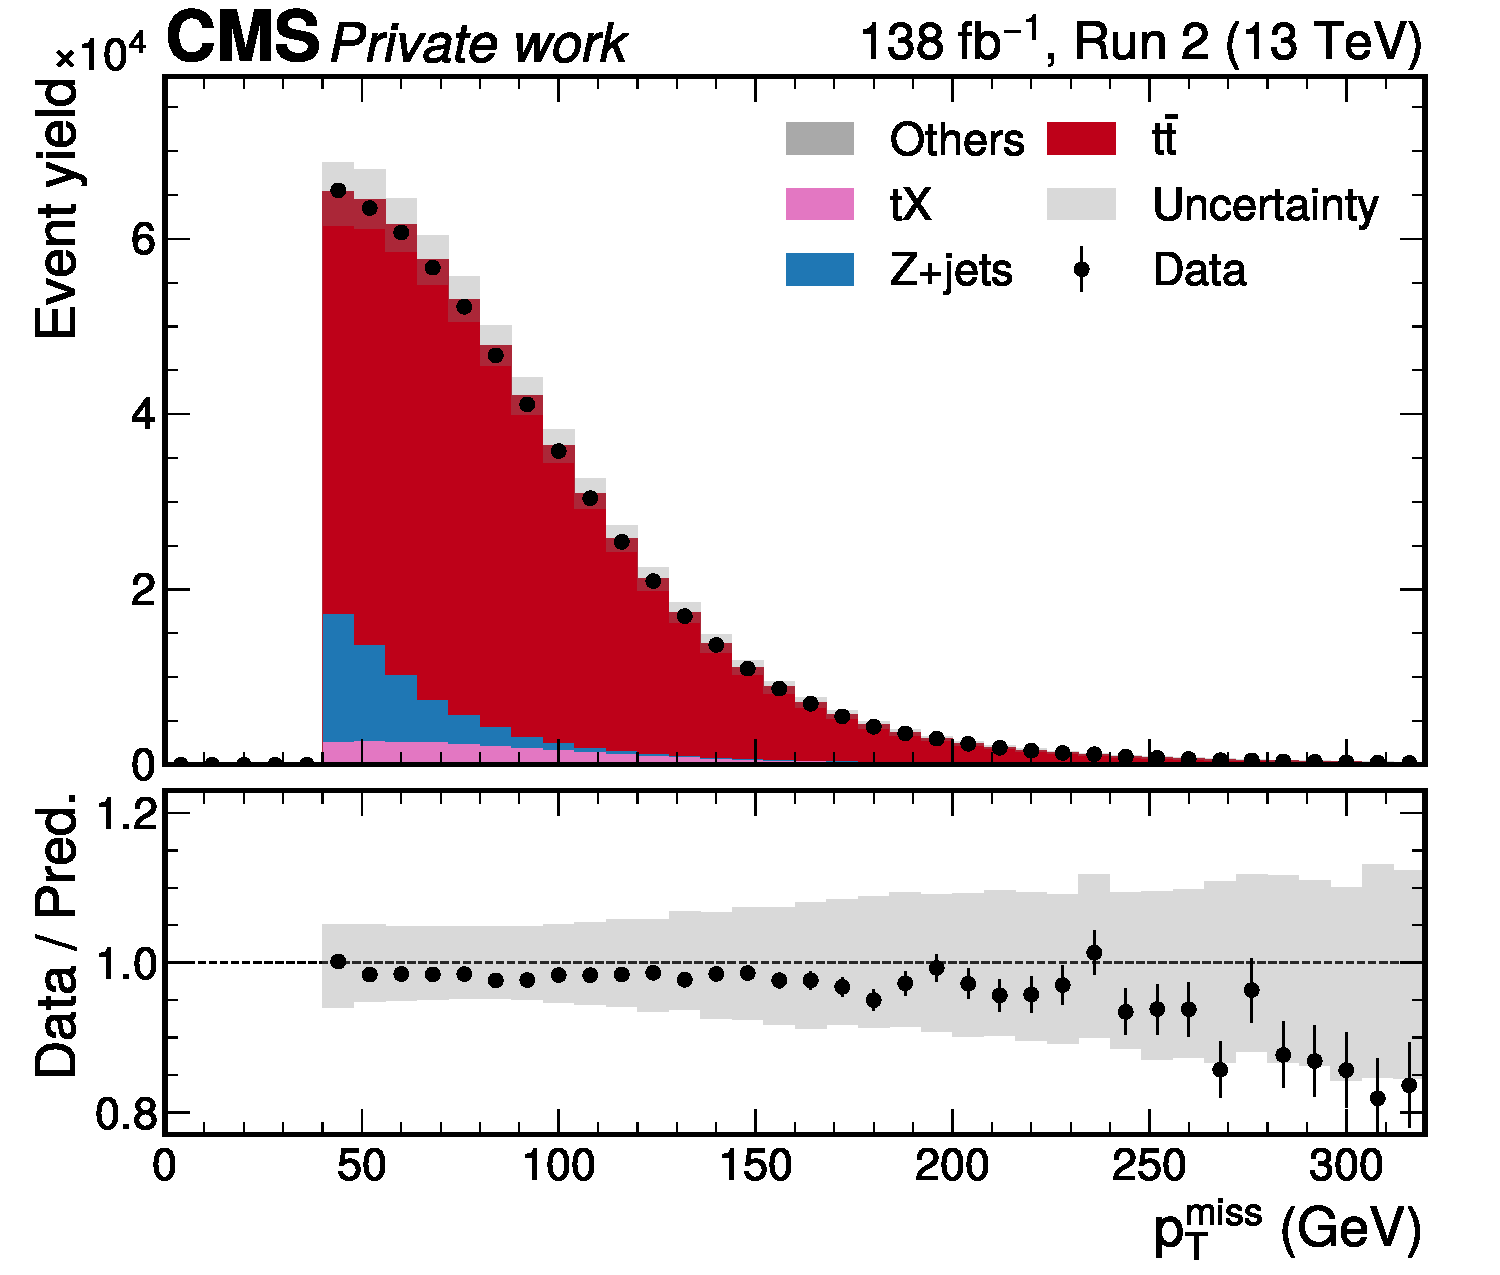
\includegraphics[width=0.49\textwidth]{figures/ah/controlplots/ReqMET/sf/METpt_ReqMET_sf.pdf}
    \hfill
    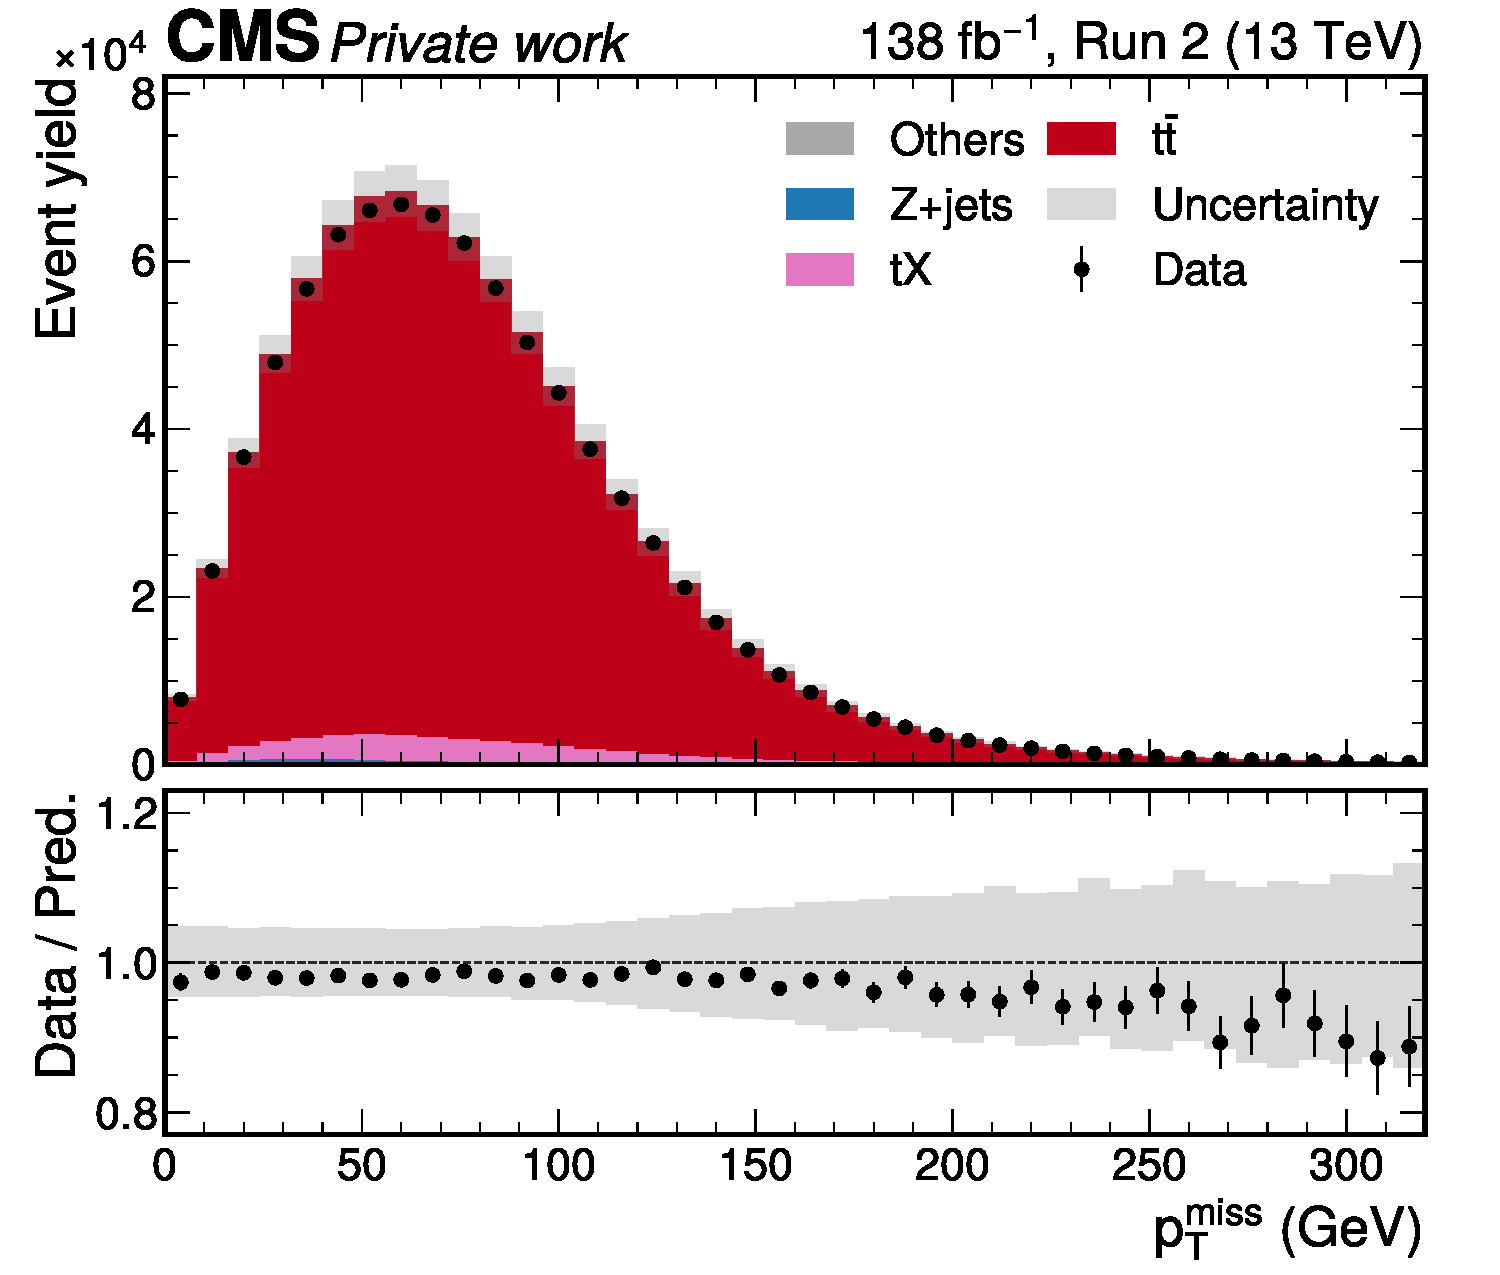
\includegraphics[width=0.49\textwidth]{figures/ah/controlplots/ReqMET/em/METpt_ReqMET_em.pdf}
    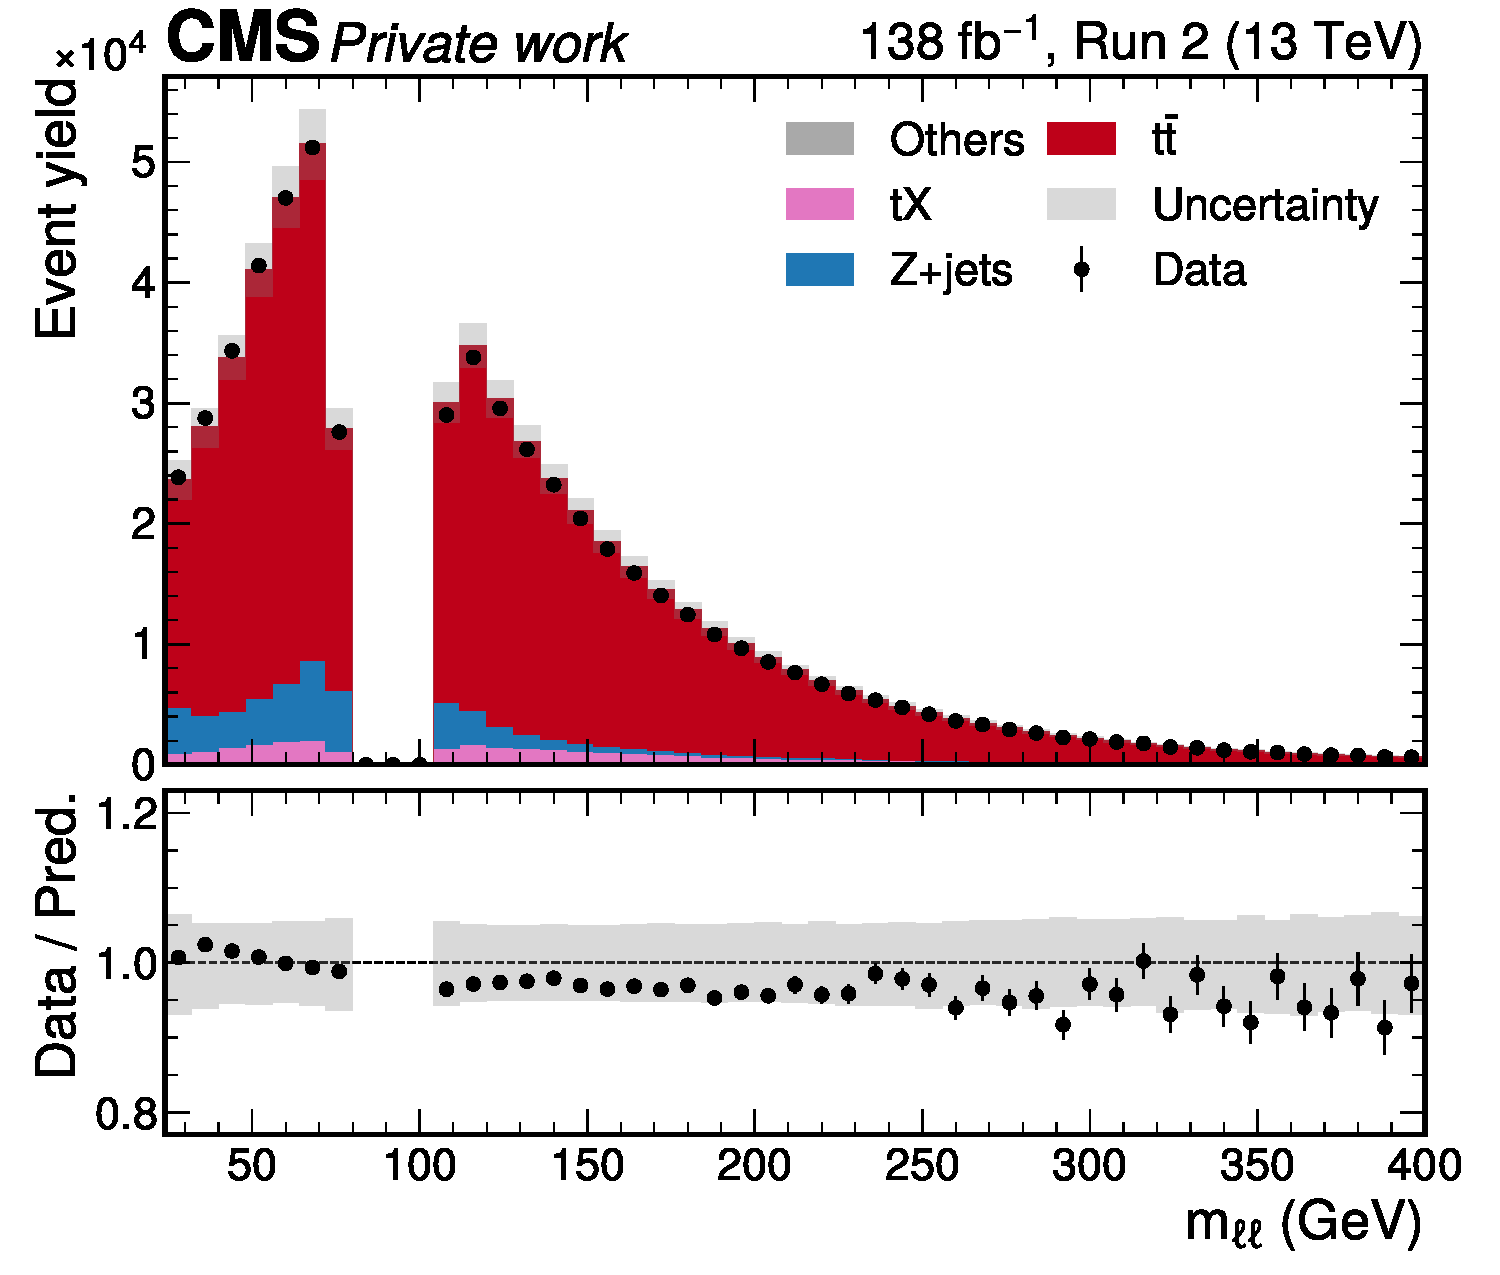
\includegraphics[width=0.49\textwidth]{figures/ah/controlplots/ReqMET/sf/mll_ReqMET_sf.pdf}
    \hfill
    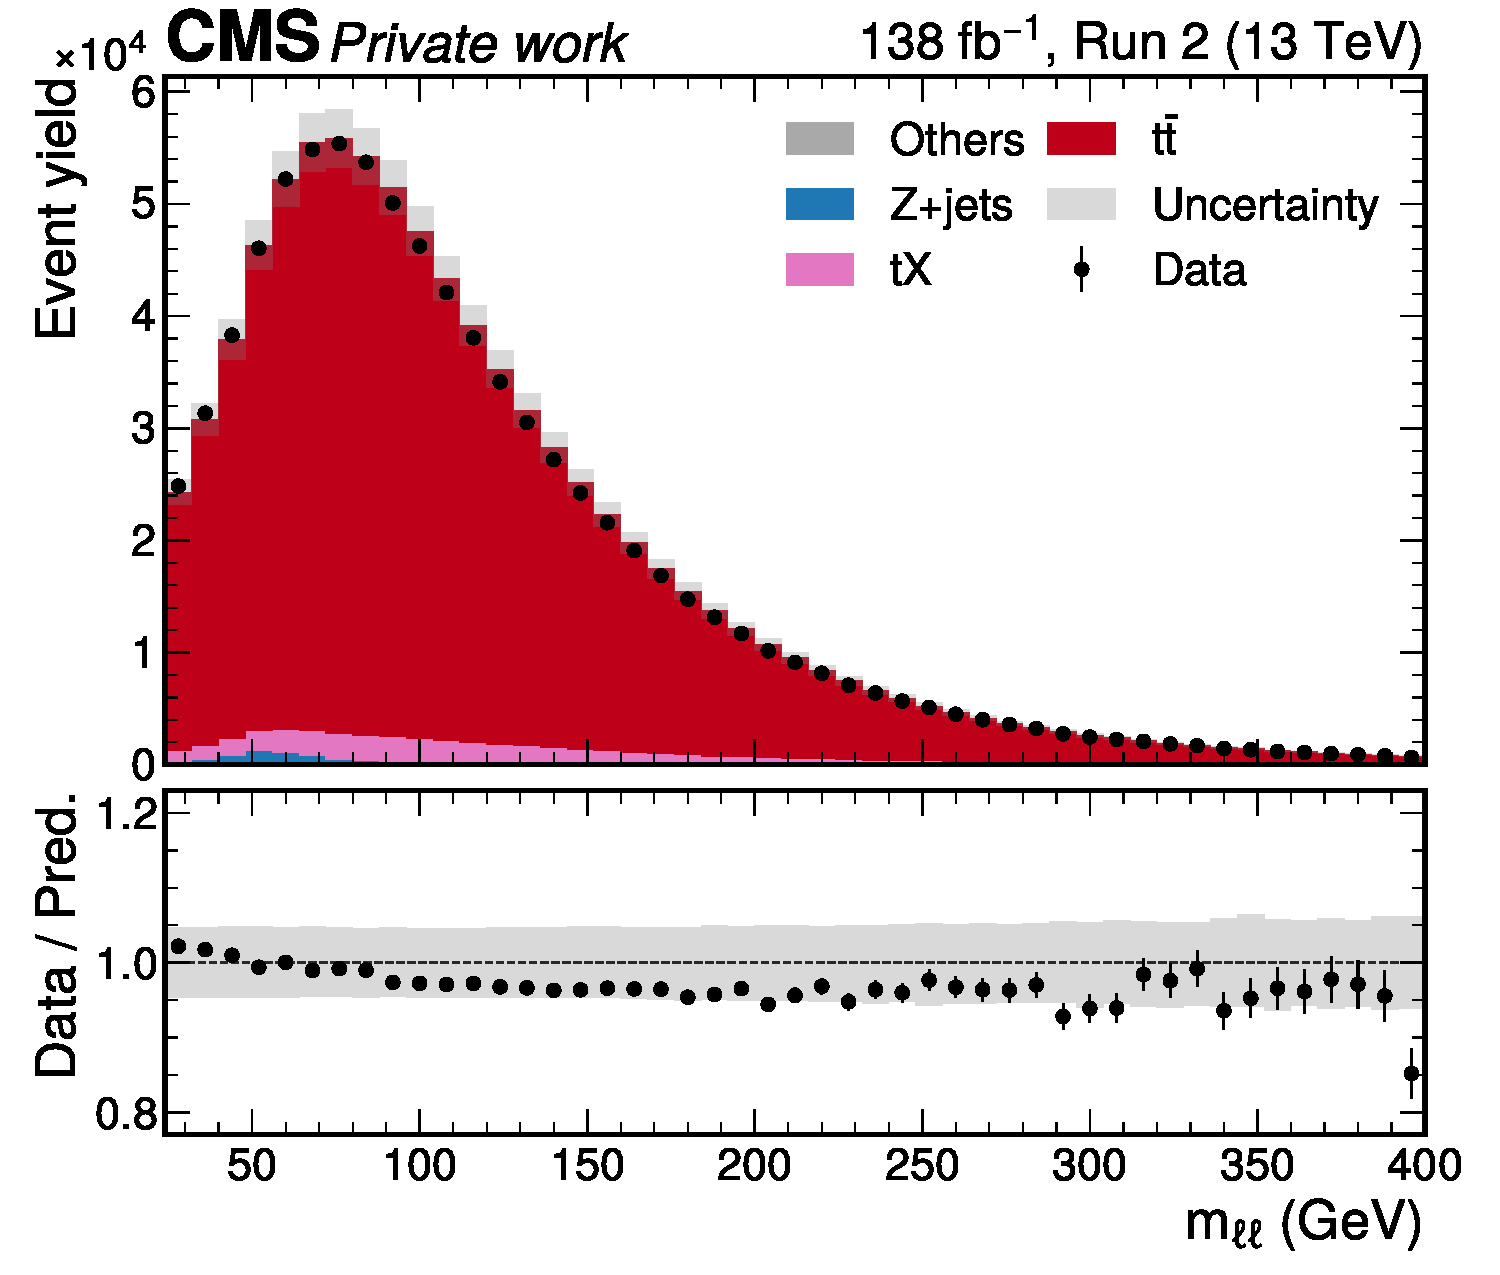
\includegraphics[width=0.49\textwidth]{figures/ah/controlplots/ReqMET/em/mll_ReqMET_em.pdf}
    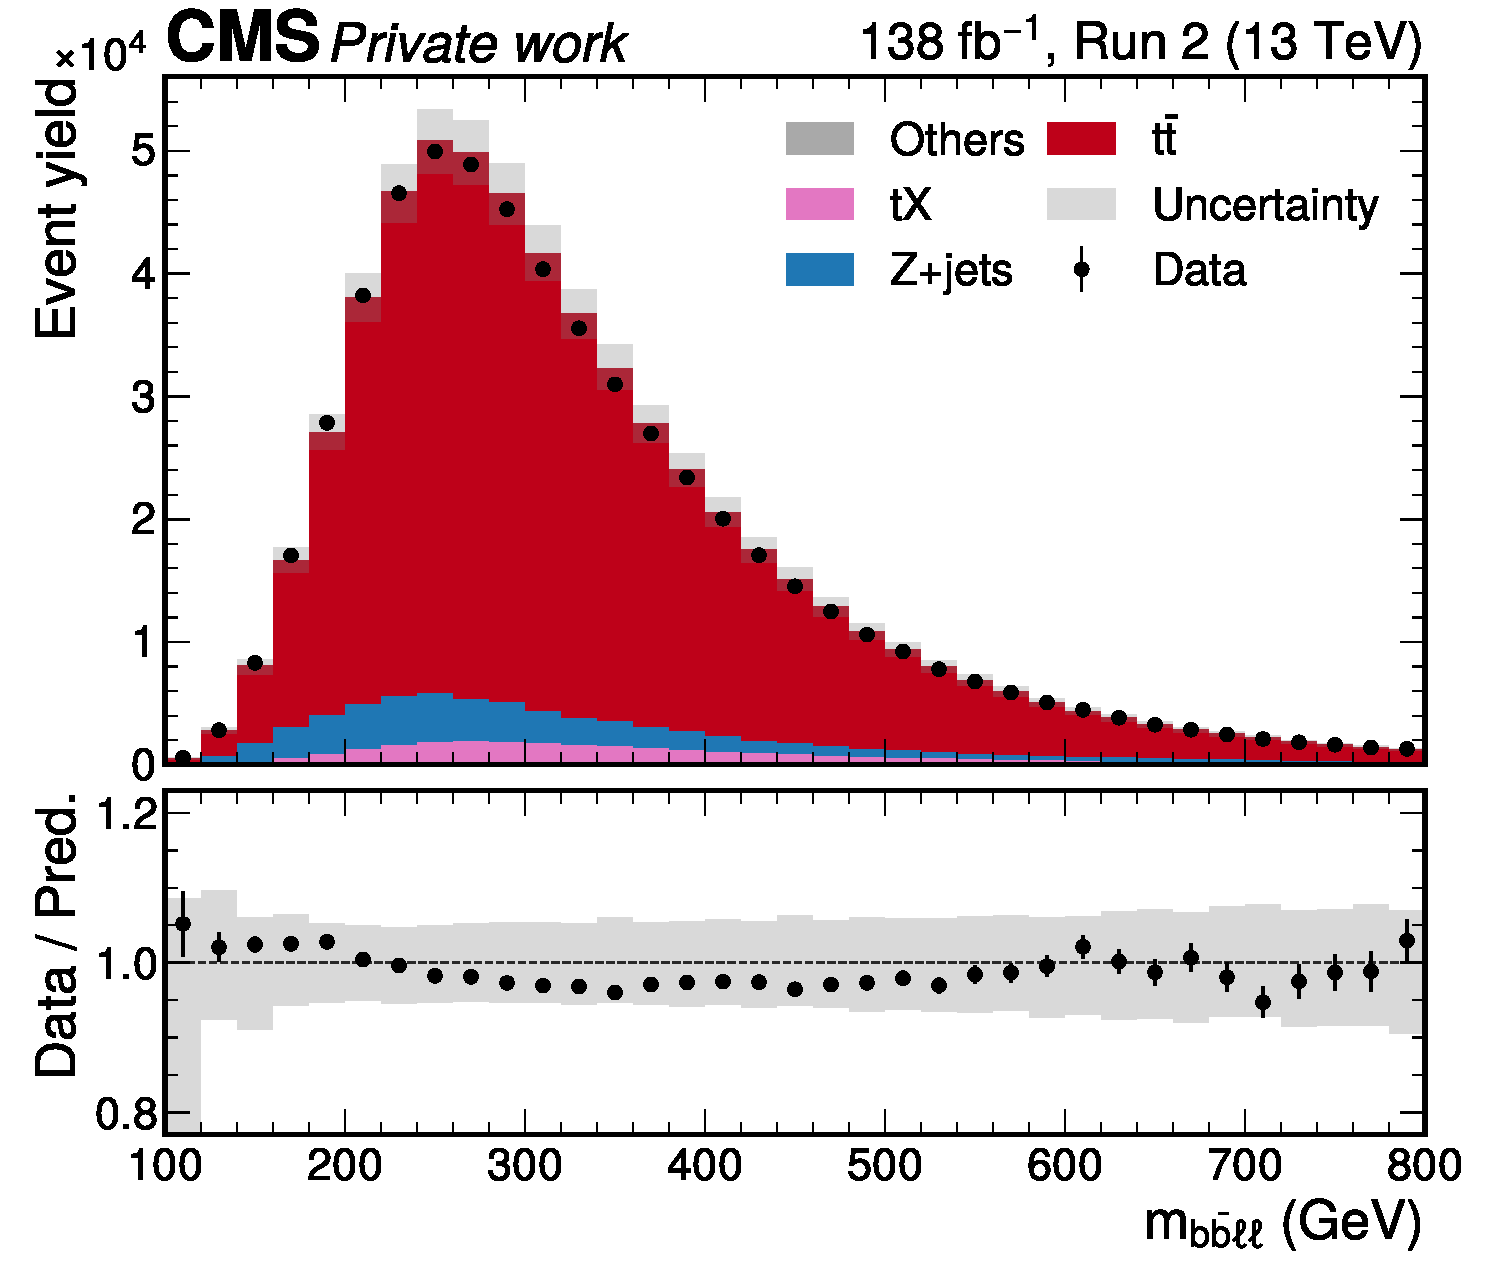
\includegraphics[width=0.49\textwidth]{figures/ah/controlplots/ReqMET/sf/mbbll_ReqMET_sf.pdf}
    \hfill
    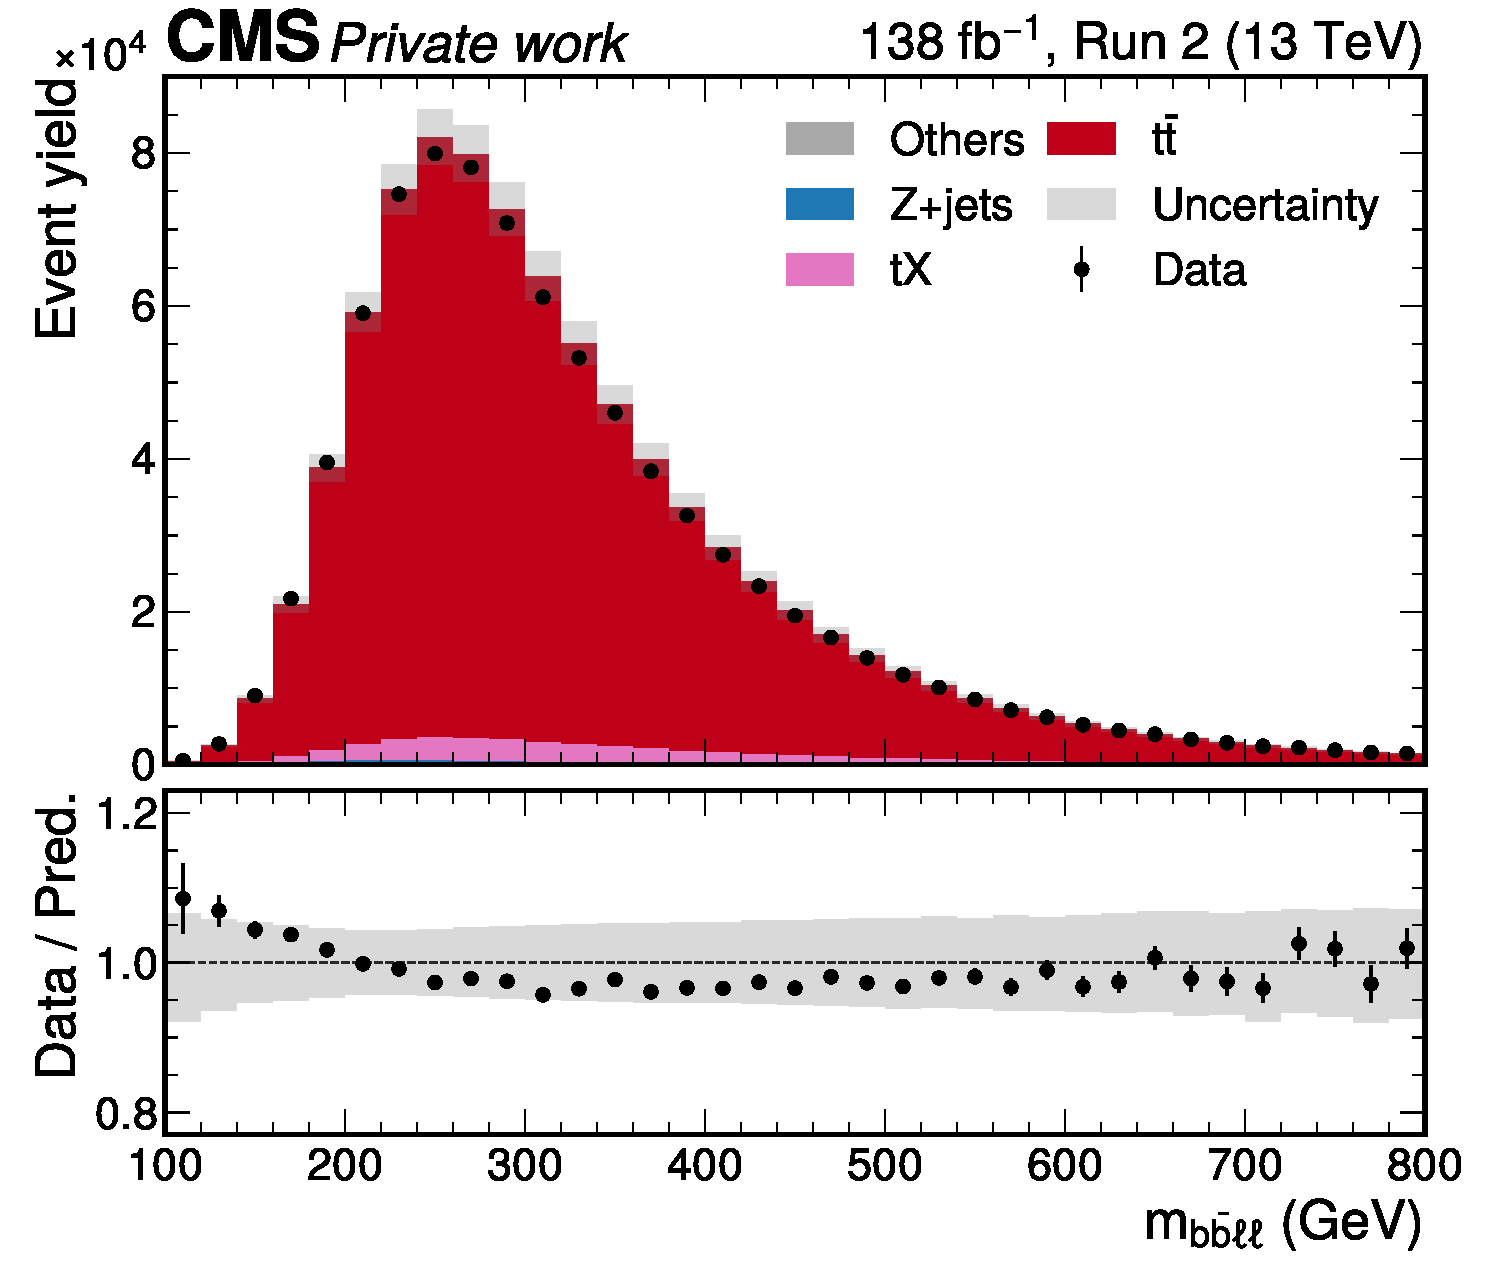
\includegraphics[width=0.49\textwidth]{figures/ah/controlplots/ReqMET/em/mbbll_ReqMET_em.pdf}
    \caption{
        \textbf{Control distributions.} Shown are the distributions of \ptmiss (top), \mll (center), and the invariant mass \mbbll of both b candidates and both leptons  (bottom) in the \ee/\mumu (left) and \emu channels (right). All figures show both data (black dots) and different simulated background processes (colored bars), as well as the total systematic uncertainty (gray band). 
    }
    \label{fig:ah:control3}
\end{figure}

\begin{figure}[!hp]
    \centering
    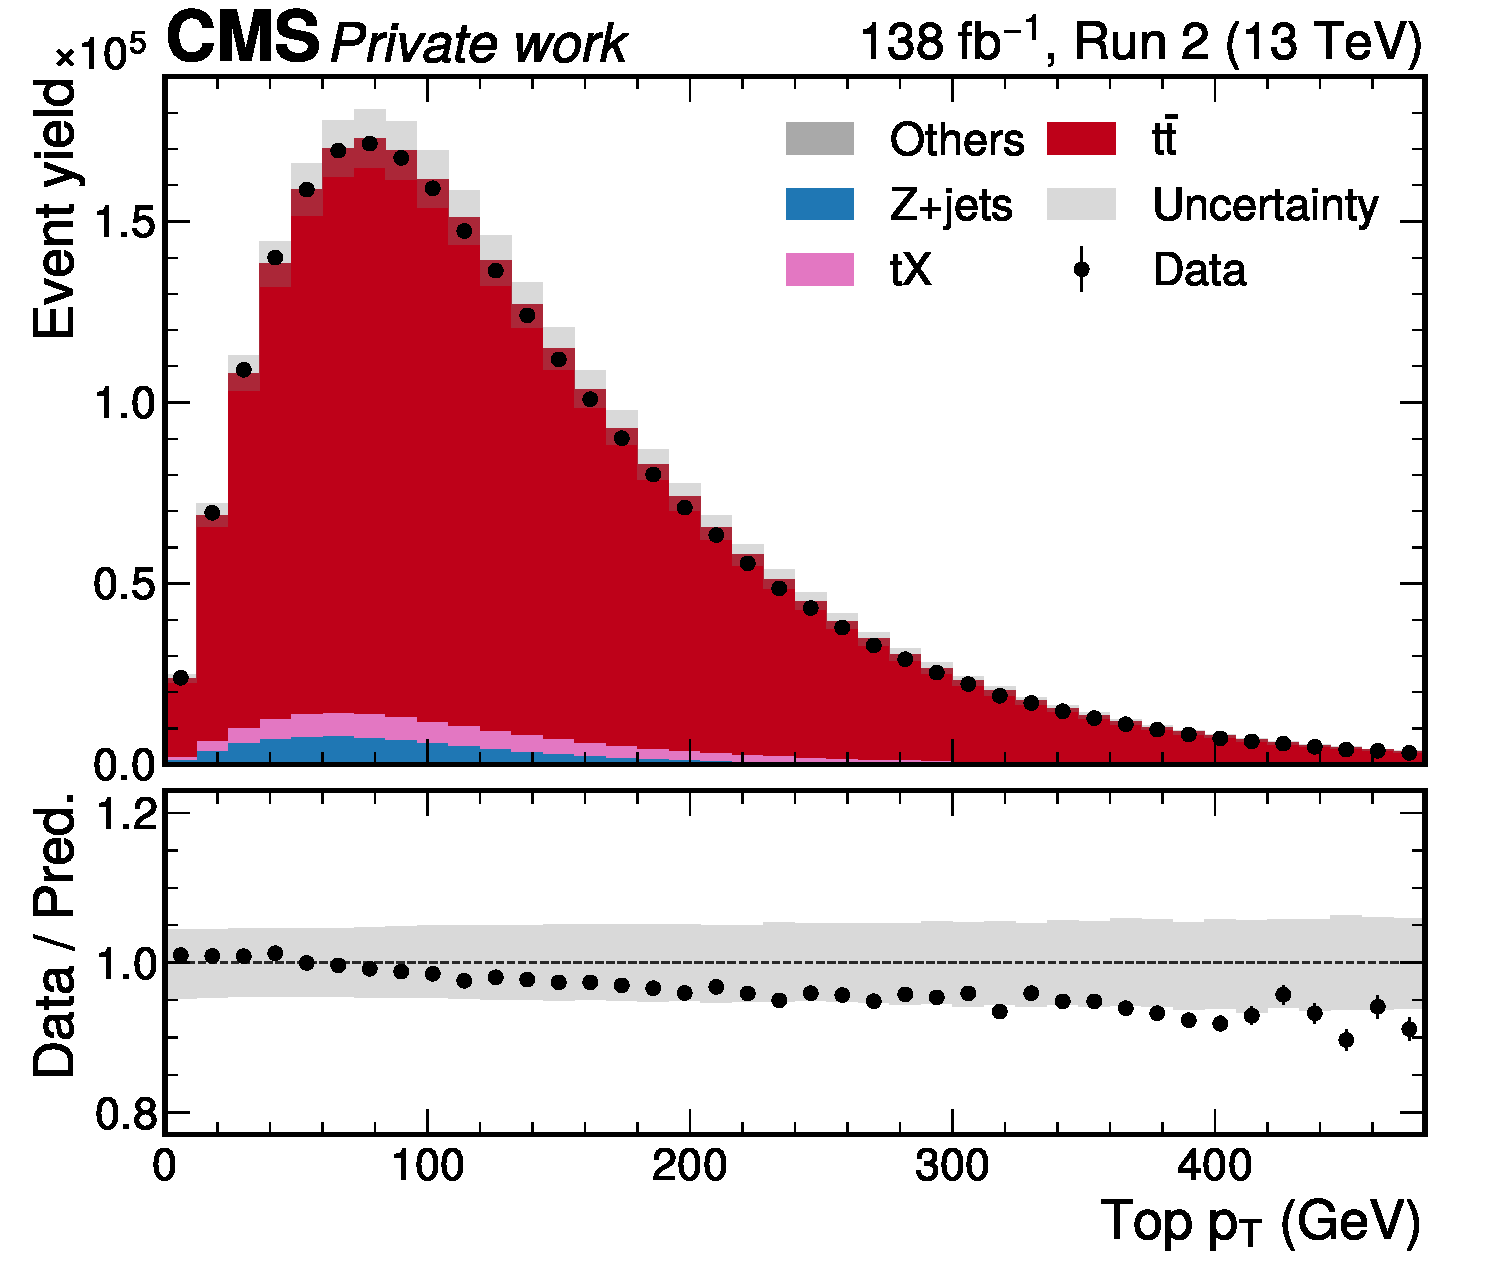
\includegraphics[width=0.49\textwidth]{figures/ah/controlplots/Reco/ll/top_pt_Reco_ll.pdf}
    \hfill
    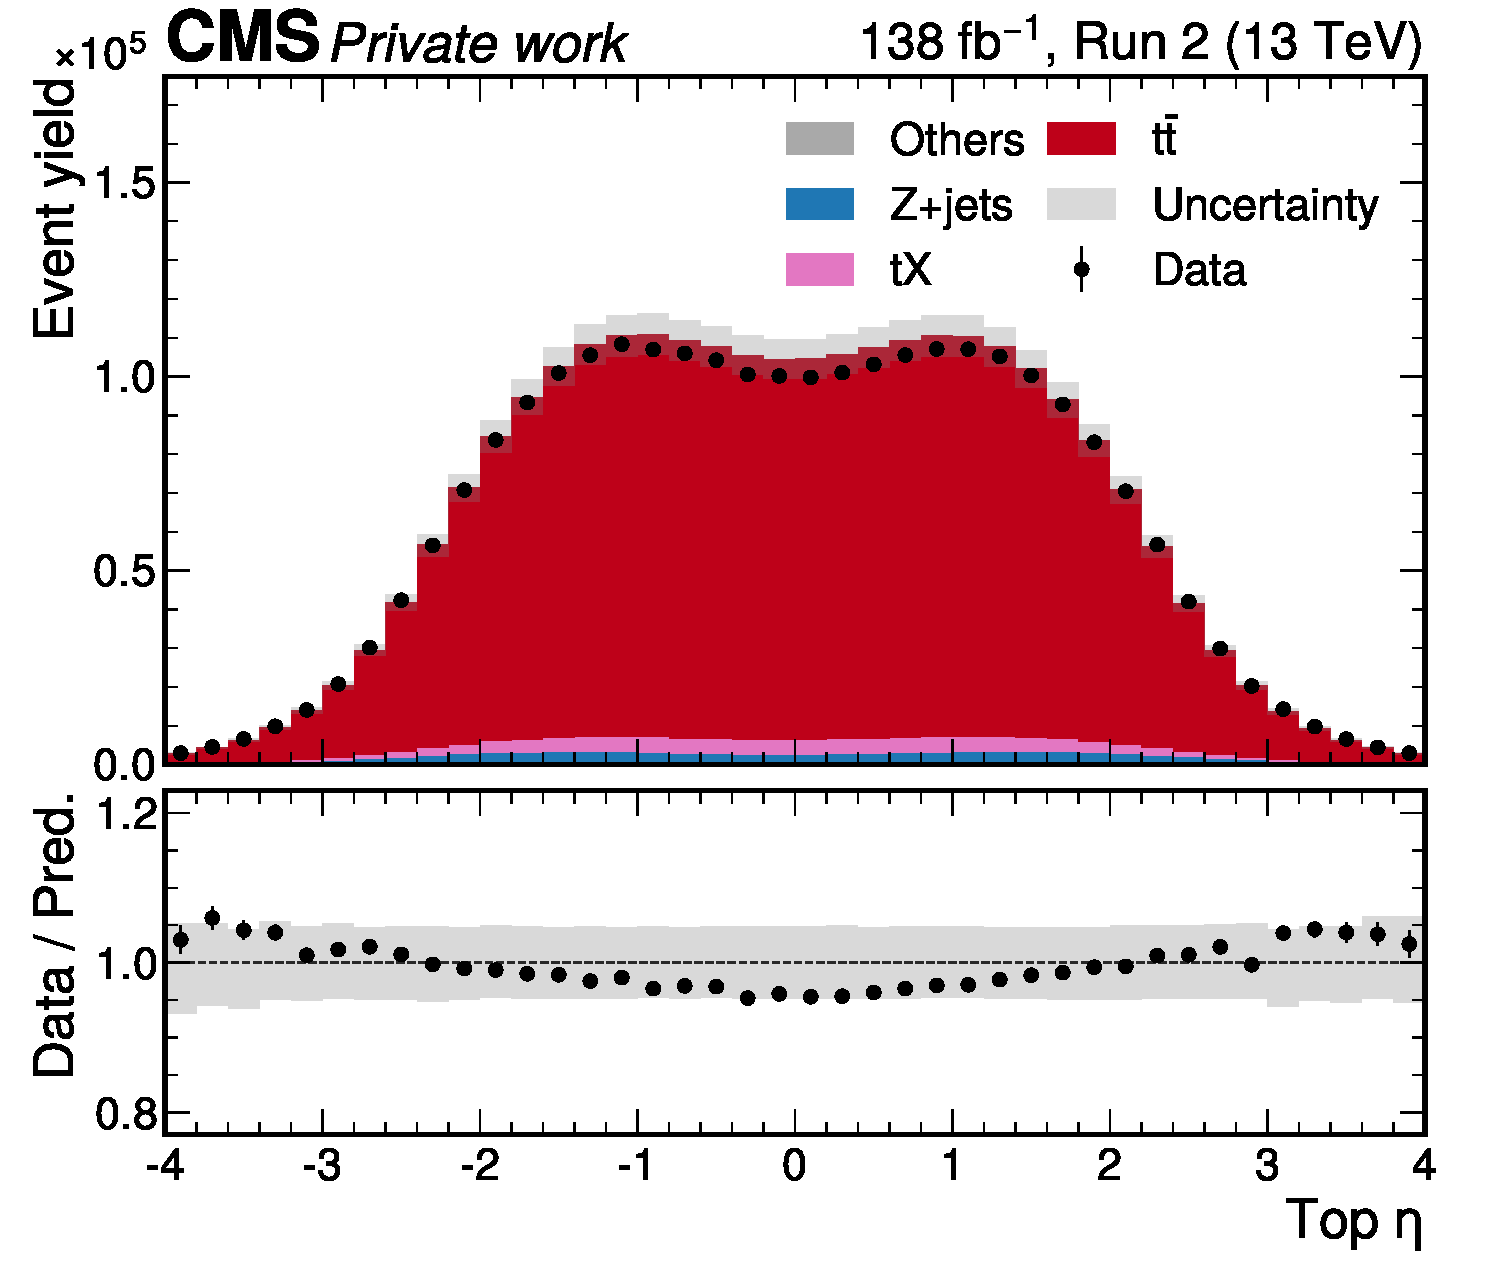
\includegraphics[width=0.49\textwidth]{figures/ah/controlplots/Reco/ll/top_eta_Reco_ll.pdf}
    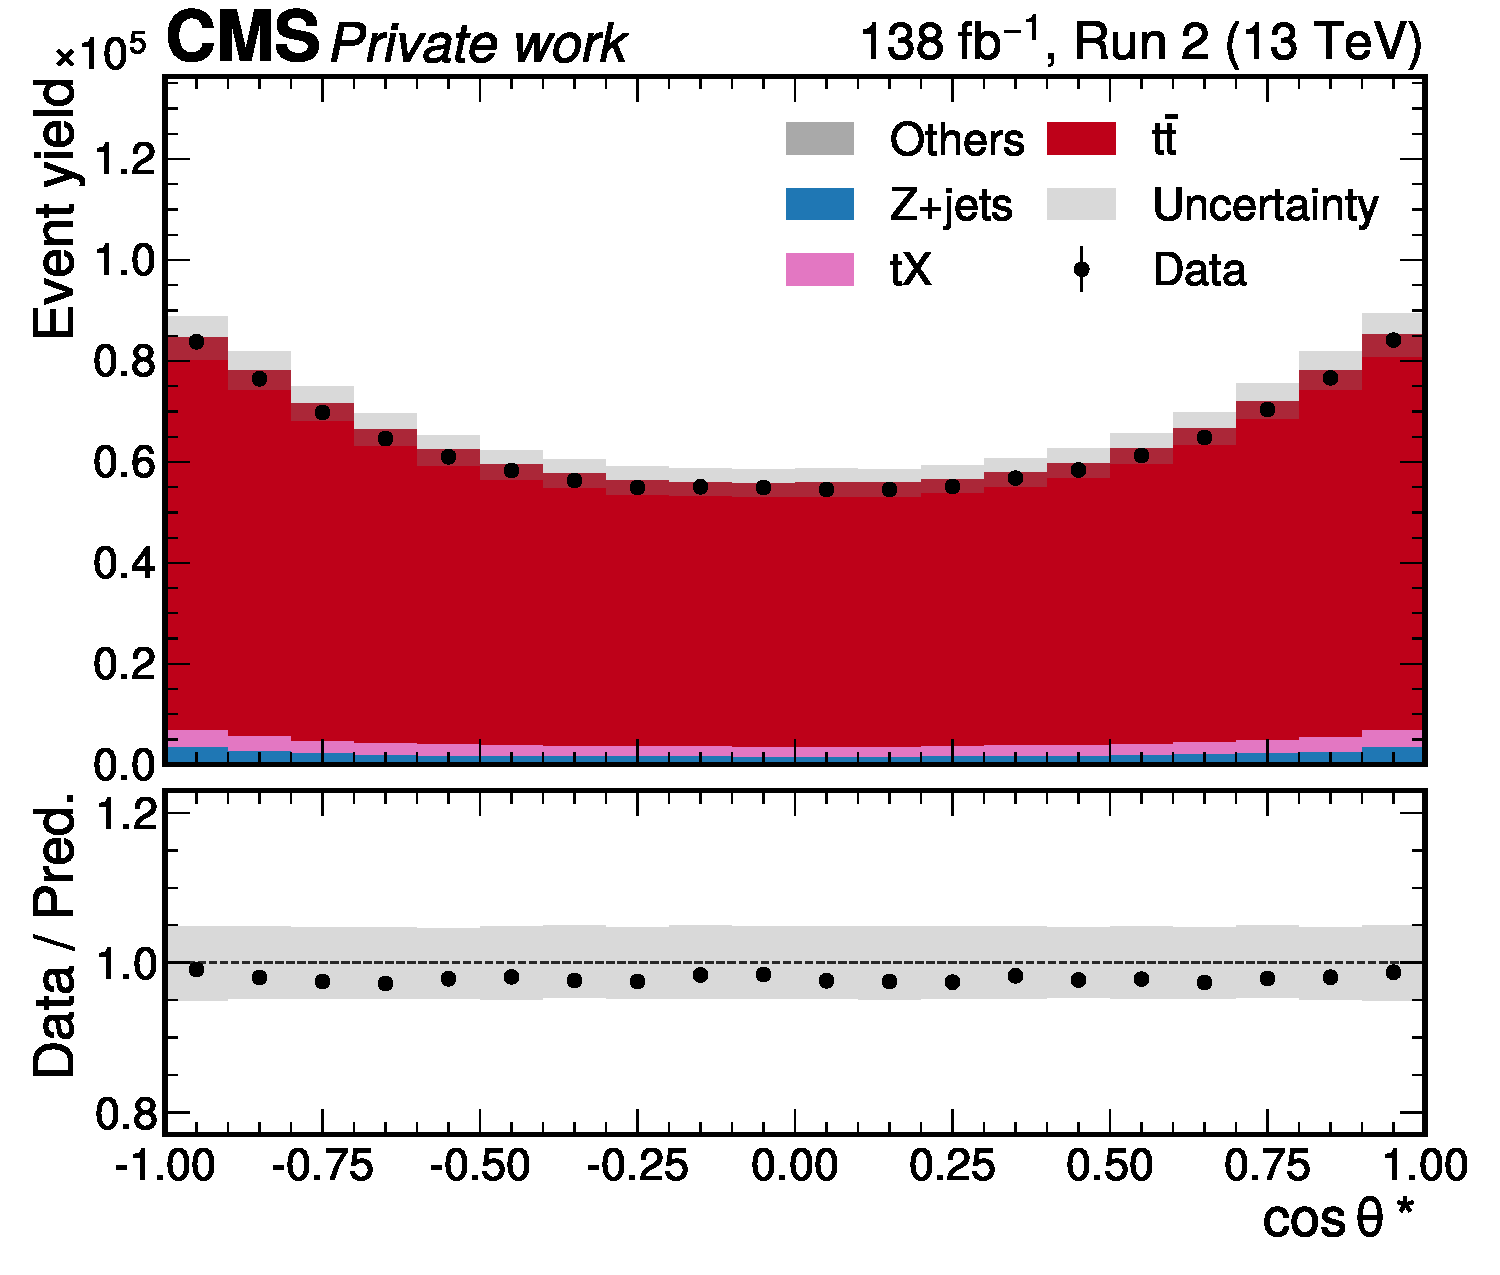
\includegraphics[width=0.49\textwidth]{figures/ah/controlplots/Reco/ll/costhetastar_Reco_ll.pdf}
    \hfill
    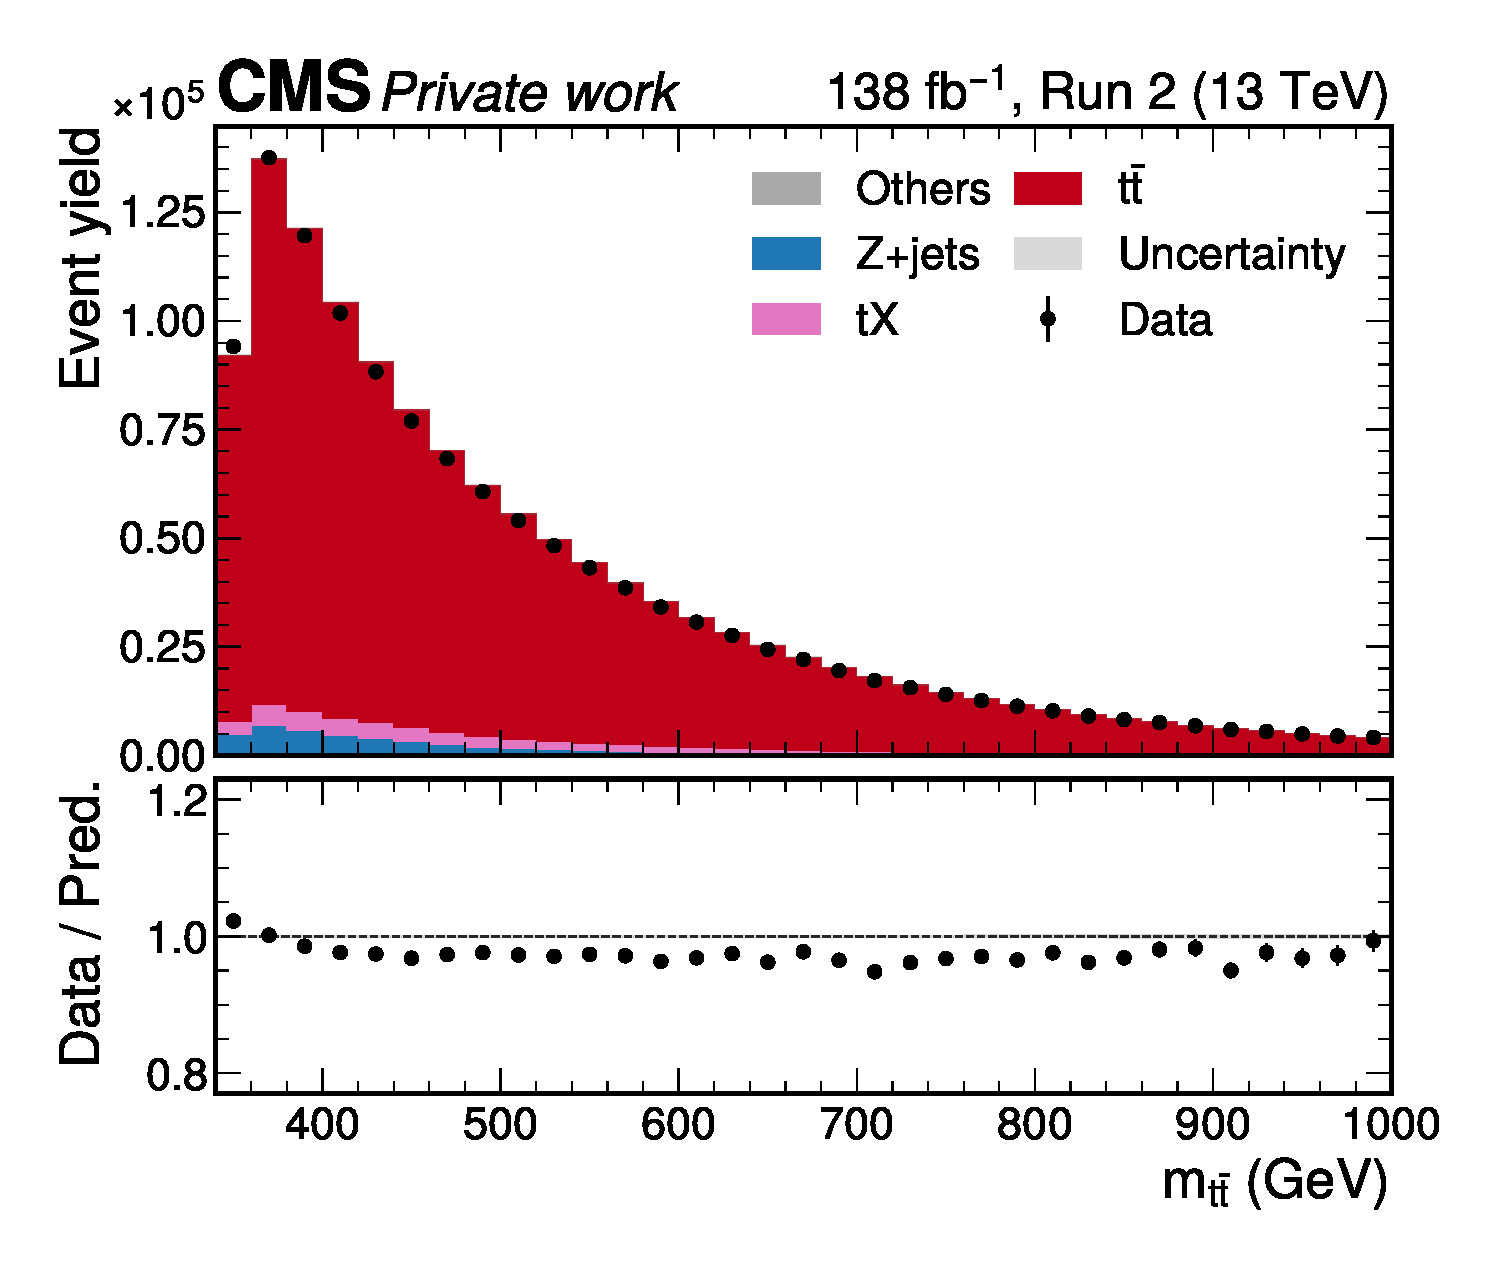
\includegraphics[width=0.49\textwidth]{figures/ah/controlplots/Reco/ll/mtt_Reco_ll.pdf}
    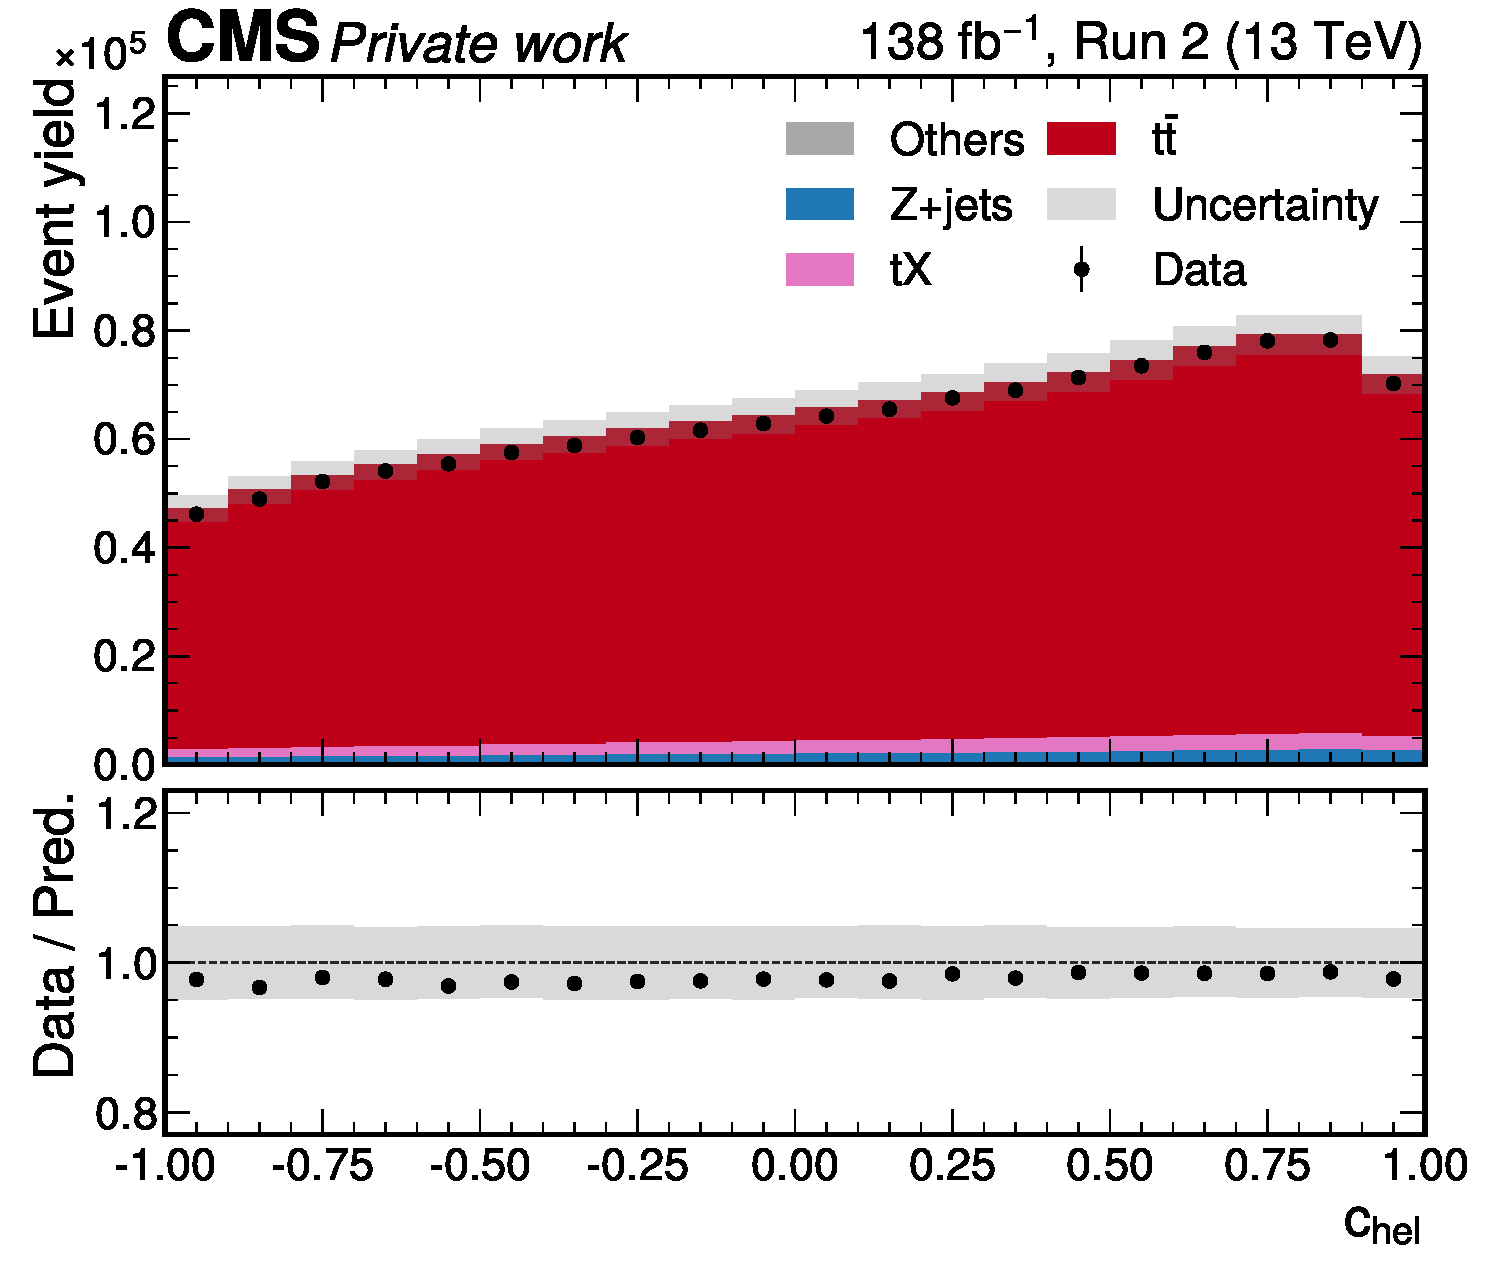
\includegraphics[width=0.49\textwidth]{figures/ah/controlplots/Reco/ll/chel_Reco_ll.pdf}
    \hfill
    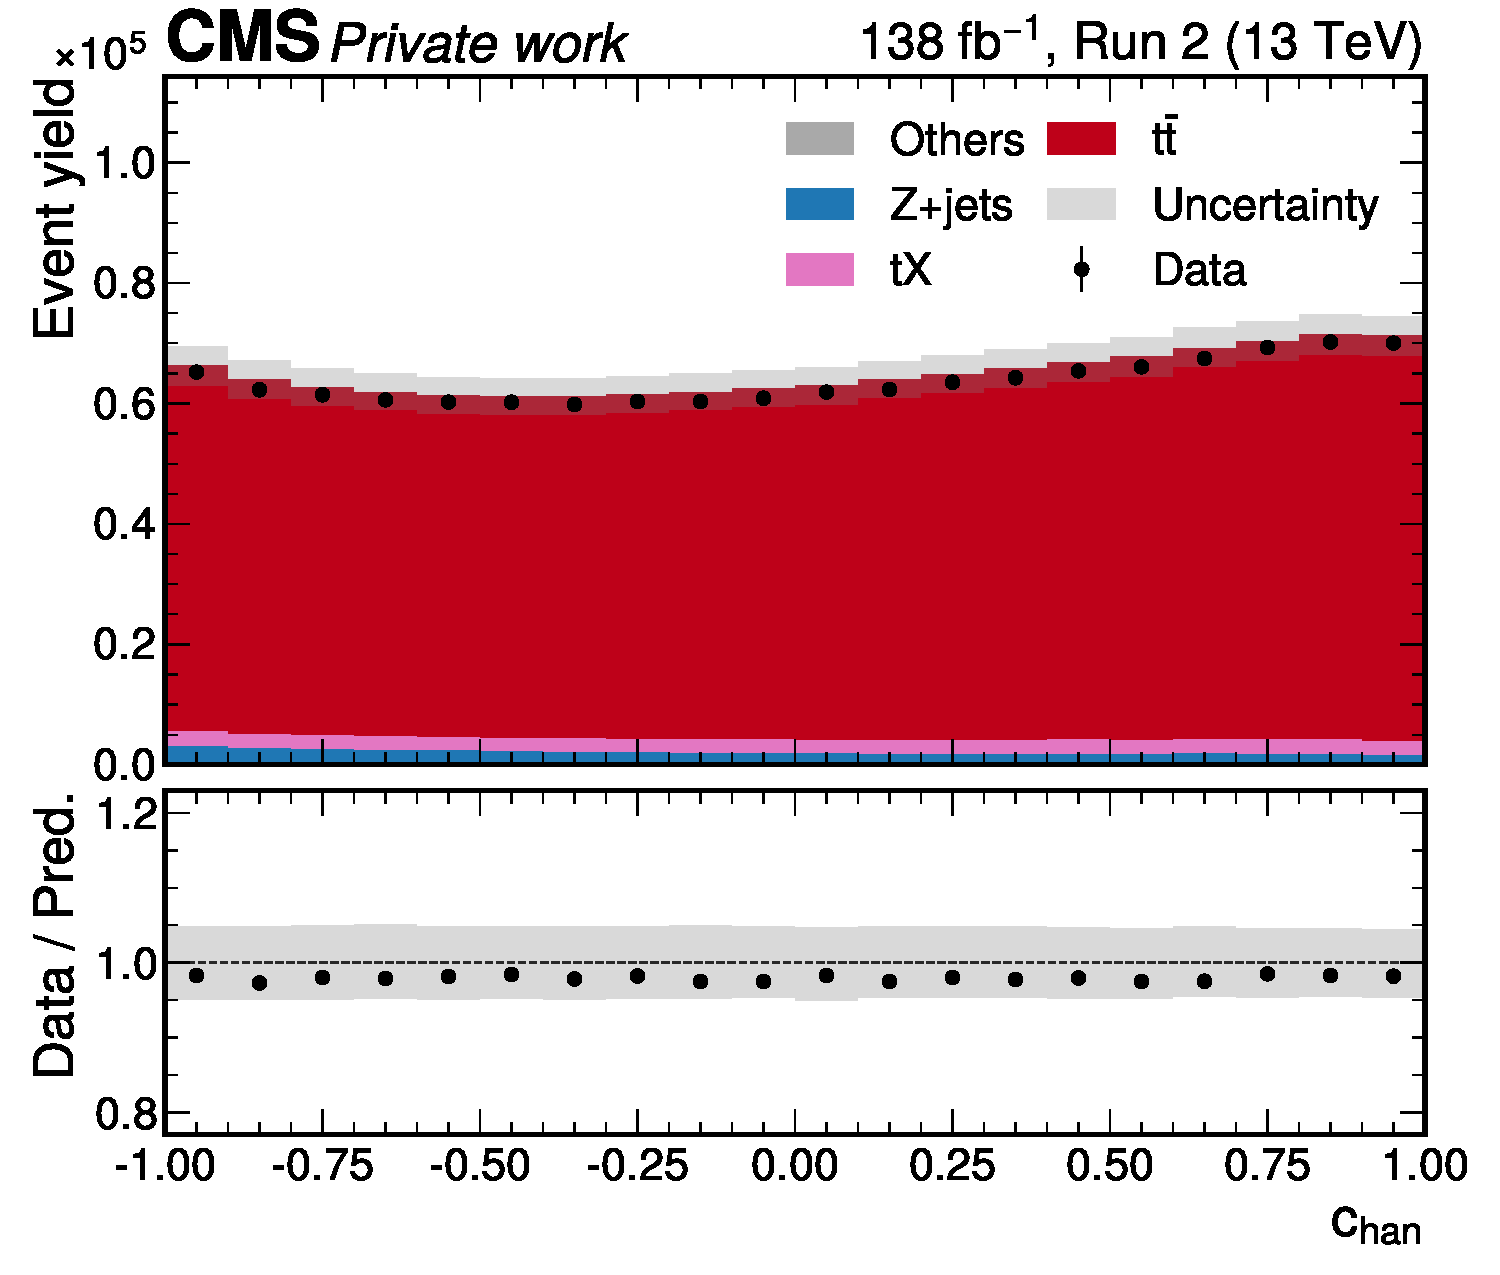
\includegraphics[width=0.49\textwidth]{figures/ah/controlplots/Reco/ll/chan_Reco_ll.pdf}
    \caption{
        \textbf{Control distributions after \ttbar reconstruction.} Shown are (from top left to bottom right) the distributions of the top quark \pt, top quark $\eta$, \mtt, \cost, \chel and \chan for the sum of all dilepton channels. All figures show both data (black dots) and different simulated background processes (colored bars), as well as the total systematic uncertainty (gray band). 
    }
    \label{fig:ah:controlttbar}
\end{figure}

The agreement between the total MC prediction, including all corrections described in \cref{sec:ah:expcorrs,sec:ah:ttbarweights}, and the observed data are presented in this section. Shown observables are lepton \pt, $\eta$, and \dphill (\cref{fig:ah:control1}); jet \pt, $\eta$, and number of jets (\cref{fig:ah:control2}); as well as \ptmiss, the invariant mass of the two leptons \mll, and the invariant mass of the two leptons and two b-tagged jets \mbbll (\cref{fig:ah:control3}). All of them are shown after all lepton, jet, b tag and \ptmiss requirements, but before the \ttbar reconstruction, summed over all analysis years, and separately for the same-flavor (\ee and \mumu) and opposite-flavor (\emu) channels, since the latter have different backgrounds and cuts.

Furthermore, different distributions resulting from the \ttbar reconstruction are shown in \cref{fig:ah:controlttbar}, this time summed also over lepton flavor. They consist of top quark \pt, $\eta$, and scattering angle \cost, as well as the three observables used for the fit \mtt, \chel, and \chan.

It can be seen that there is a slight but consistent over-prediction of the background normalization compared to the data in almost all distributions. Furthermore, there is a slight slope in the ratio of data and simulation yields in the \pt of leptons, jets or the reconstructed top quarks. This is likely a result of the well-known top quark \pt mismodeling at the LHC, which is not fully removed by NNLO QCD corrections as used here~\cite{CMS:TOP-16-008,CMS:TOP-17-014}. Further discrepancies are found for high values of \abseta and for large number of jets, both of which are covered by systematic uncertainties.

Finally, the three-dimensional \mttchelchan distribution used for the statistical analysis is shown before the fit, including all systematic uncertainties, in \cref{fig:ah:prefit_ll}. A notable excess of the data compared to the prediction is observed for low values of \mtt, consistent with the excess seen in the one-dimensional \mtt distribution (\cref{fig:ah:controlttbar}) and in the related observables \mll and \mbbll (\cref{fig:ah:control3}). The excess is stronger for large values of \chel as seen from the multi-dimensional binning, while no trend can be seen by eye regarding \chan.

\begin{figure}[t]
    \centering
    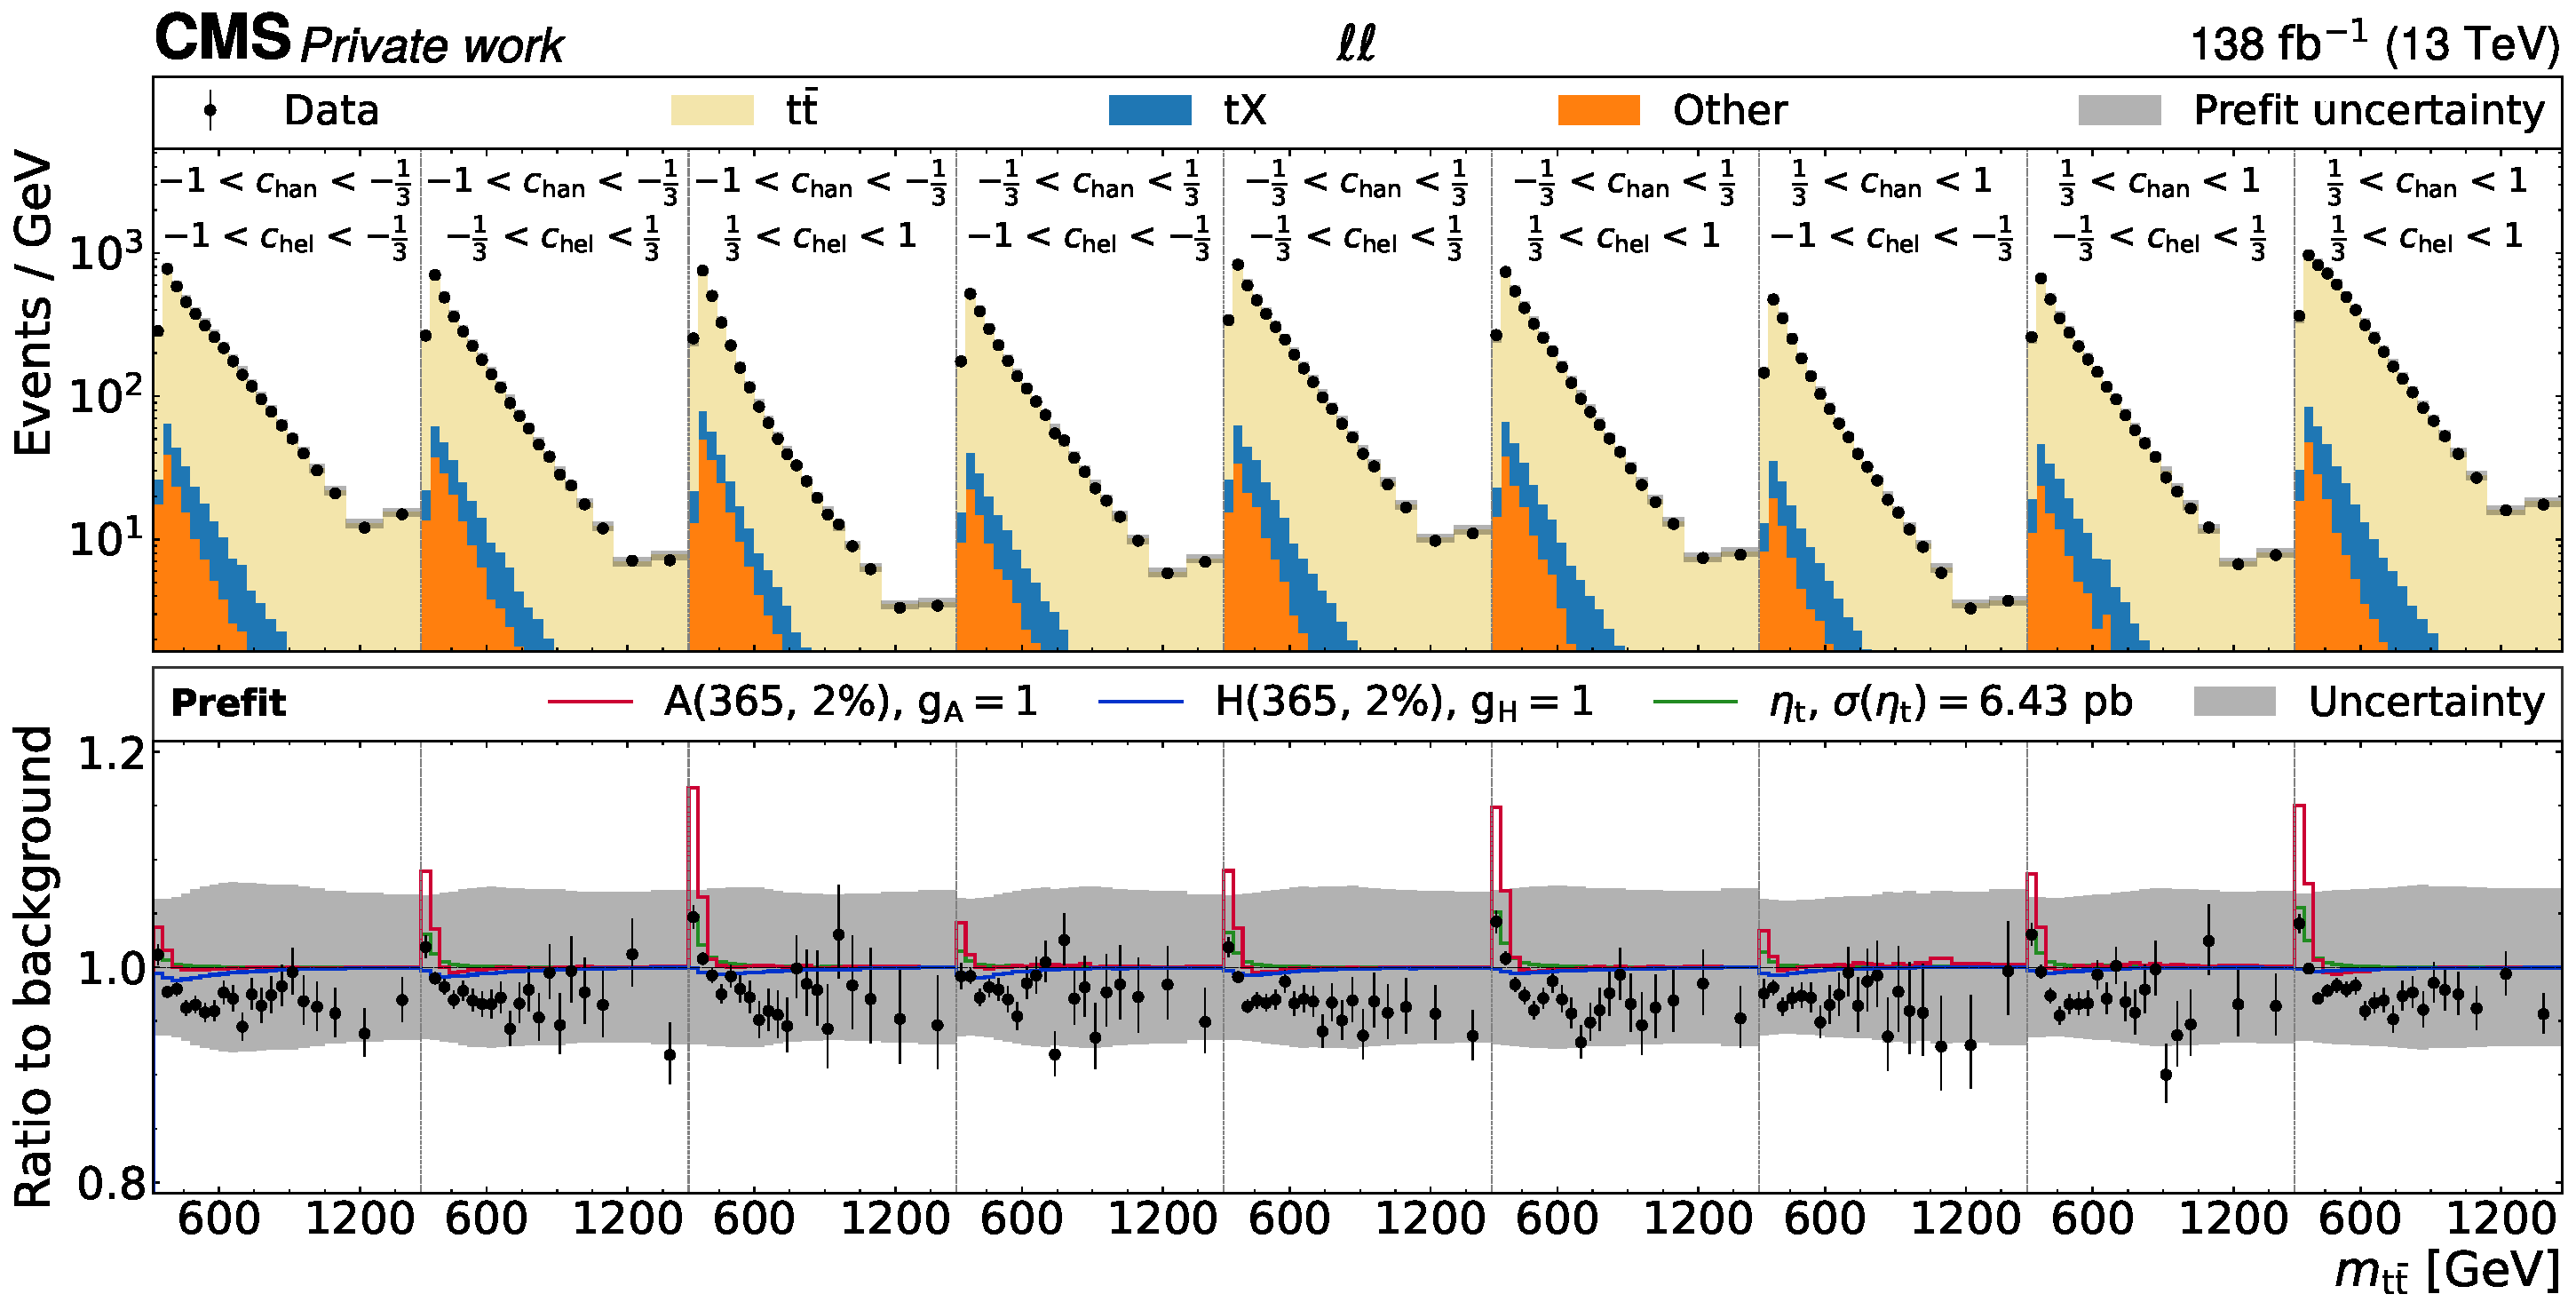
\includegraphics[width=0.99\textwidth]{figures/ah/prepost/A_m365_w2p0__H_m365_w2p0_fit_p_ll_run2_both.pdf}
    \caption{
        \textbf{Prefit distributions of \mttchelchan.} The unrolled three-dimensional distribution in \mtt, \chel and \chan as used for statistical analysis before the fit to the data, summed over all years and lepton flavors. The upper panel shows the sum of the background simulation (colored bars) and the observed data (black dots), while the lower panel shows the ratio of the data to the prediction, with different signals overlaid: A (red) and H (blue), both for $\mAH = \SI{365}{\GeV}$ and $\wAH/\mAH = 2\%$, and \etat (green). \textit{Figure adapted from \citere{CMS:HIG-22-013-PAS}}.
    }
    \label{fig:ah:prefit_ll}
\end{figure}

%\section{Extraction of non-perturbative effects in \ttbartitle}
%\label{sec:ah:etat}

\section{Interpretation of the excess}
\label{sec:ah:excess}

\subsection{Extraction of \ttbartitle bound state effects}
\label{sec:ah:etat}

The prefit excess visible in \cref{fig:ah:prefit_ll} is interpreted in terms of a pseudoscalar \ttbar bound state by performing a signal+background fit with \etat as the signal, as defined in \cref{sec:theory:etat}. The POI in the fit is \sigetat, the cross section of the \etat model, which can be understood as the difference between the data and the fixed-order perturbative QCD (FO pQCD) background prediction. It is measured to be

\begin{equation}
    %\sigetat = 8.8^{+1.2}_{-1.4} \, \si{\pb}.
    \sigetat = 8.7 \pm 0.5 (\text{stat}) \pm 1.0 (\text{syst}) \, \si{\pb} = 8.7 \pm 1.1  \, \si{\pb}.
\end{equation}

The statistical and systematic component of the uncertainty are estimated as described in \cref{sec:methods:stat}. The significance of the result compared to a background-only hypothesis, i.e. without a bound state, is more than five standard deviations.

The result is of a similar order of magnitude as the prediction of \SI{6.43}{\pb} given in \citere{Fuks:2021xje}, obtained by fitting the results of an NRQCD calculation from \citere{Sumino:2010bv}, though this result is not one-to-one comparable since it considers only the range of $\mtt \in [338, 350] \, \si{\GeV}$. It should be noted that the results of \citere{Sumino:2010bv} (as well as the newer ones in \citere{Garzelli:2024uhe})  where obtained by using NLO hard functions for the NRQCD calculations, and moving to NNLO might give a significant increase in cross section, by analogy to the difference in NNLO and NLO cross sections for the \ttbar continuum. Furthermore, the NRQCD approach employed in these calculations considers only the ground state wavefunction of the bound \ttbar system, and independent calculations have shown that including contributions from excited states could increase the cross section by orders of 15--20\%~\cite{Llanes-Estrada:2024phk,dEnterria:2025ecx}.

\begin{figure}[p]
    \centering
    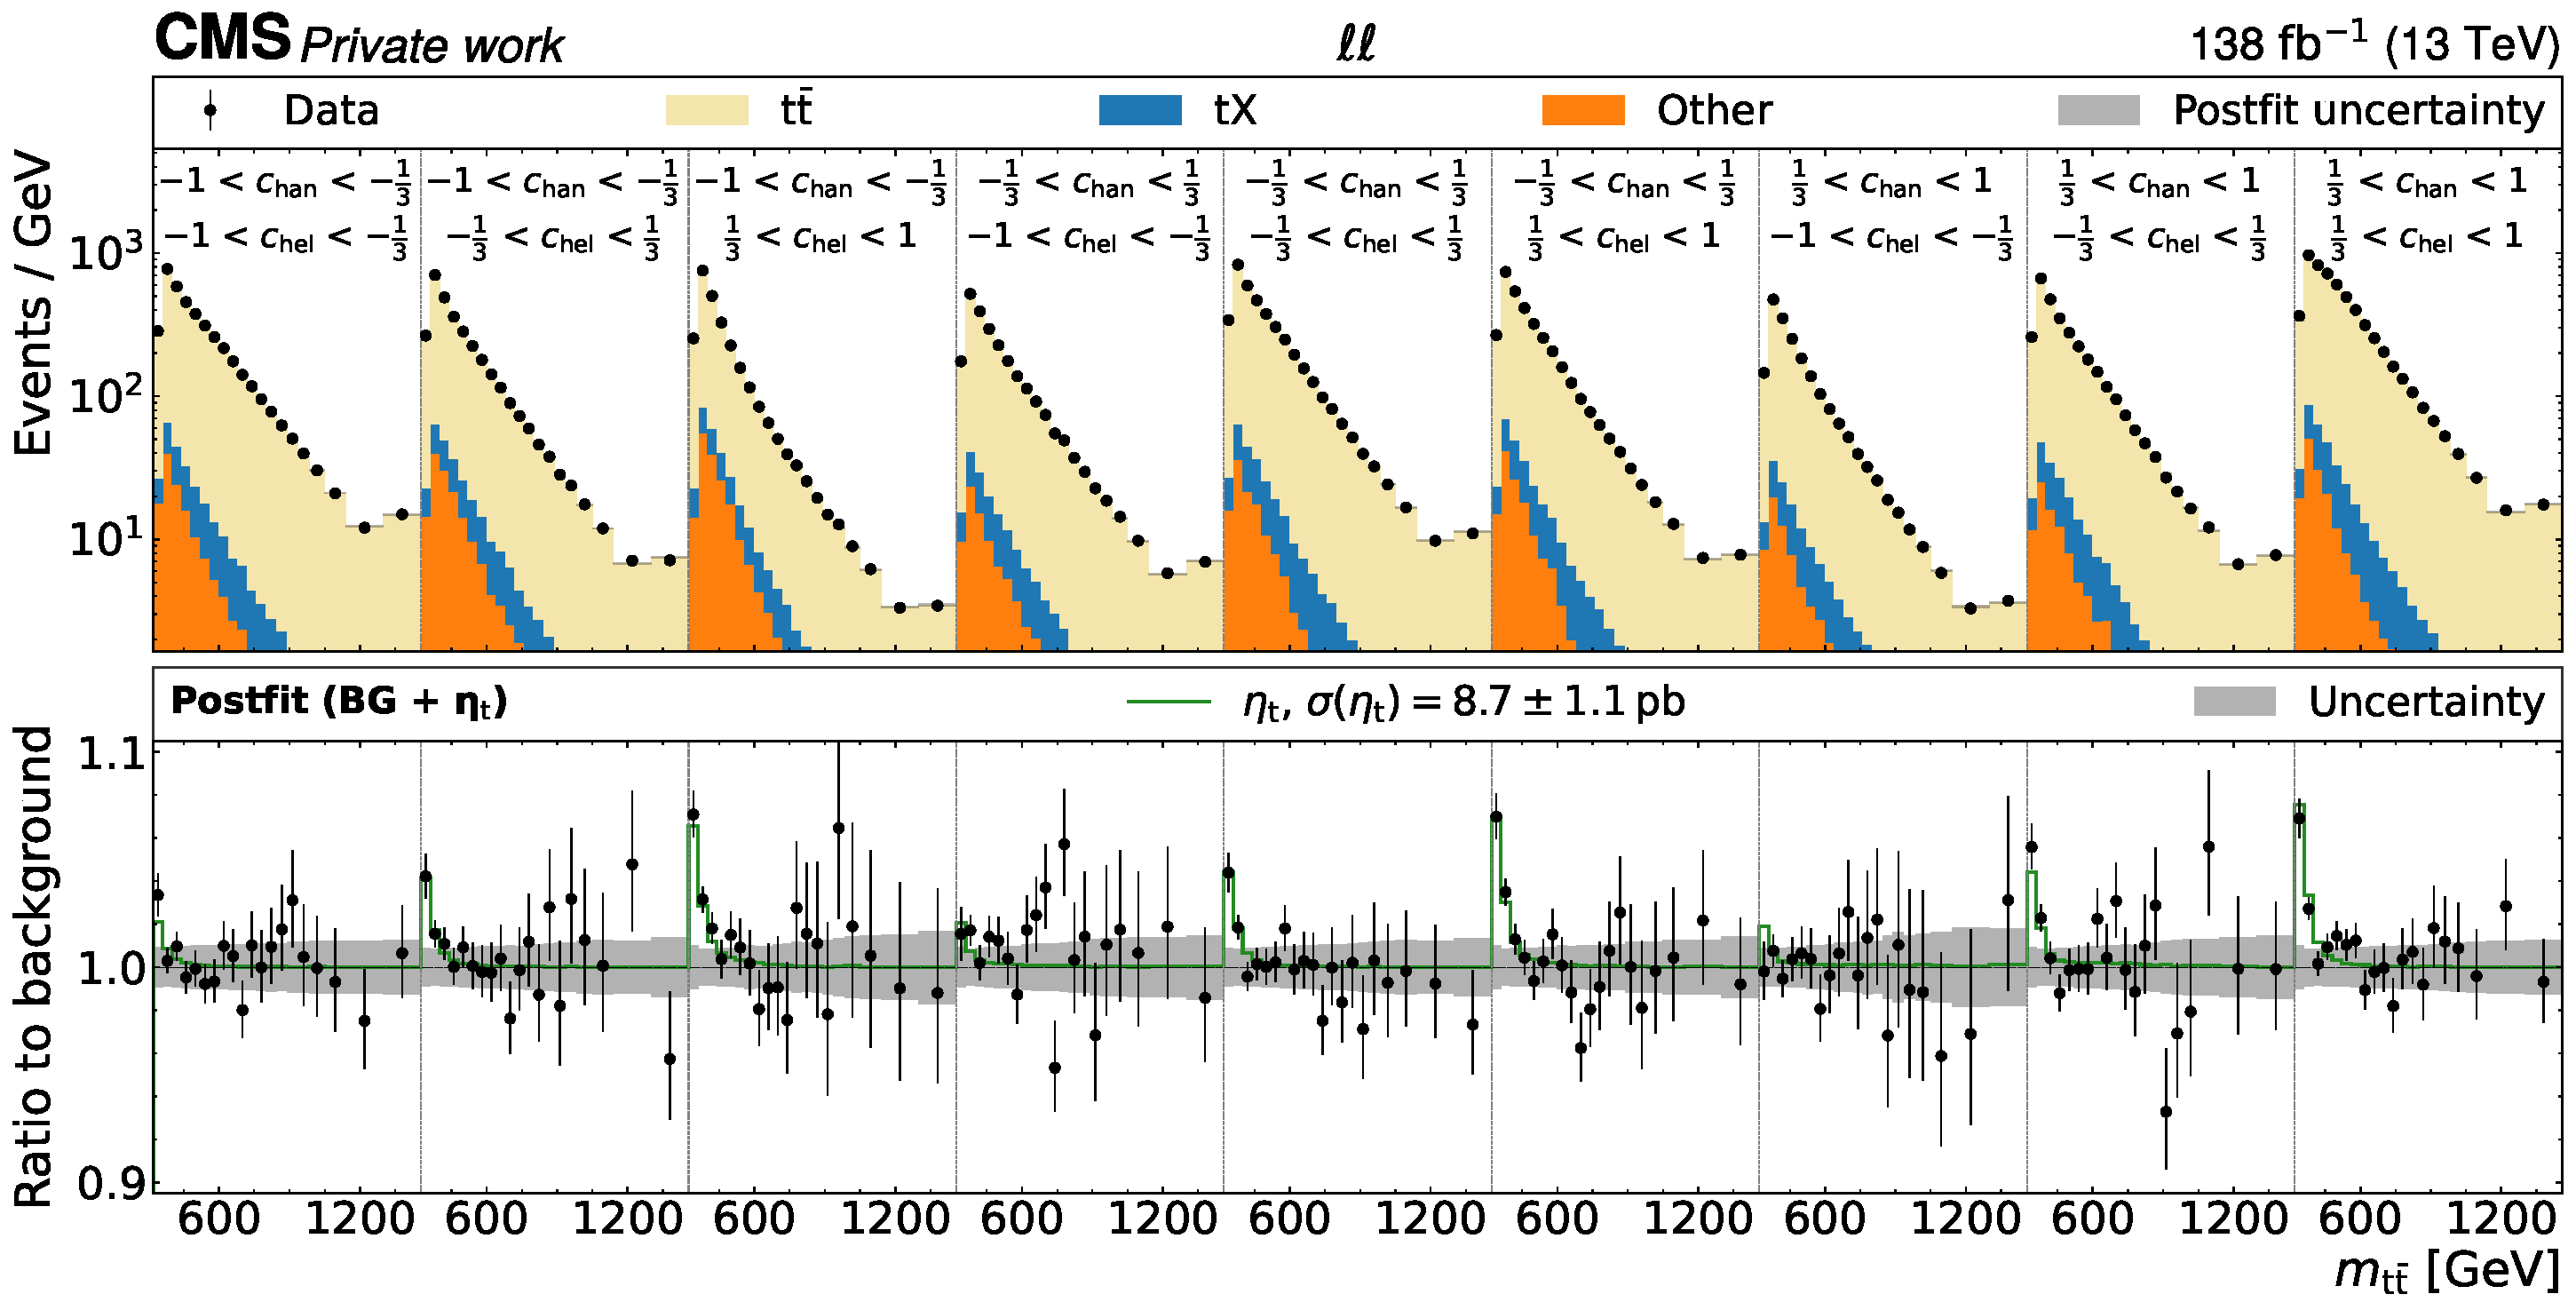
\includegraphics[width=0.99\textwidth]{figures/ah/prepost/EtaT_fit_s_ll_run2_both.pdf}
    \caption{
        \label{fig:ah:postfit_etat_ll}
        \textbf{Postfit distributions of \mttchelchan for the \etat fit.} The unrolled three-dimensional distribution in \mtt, \chel and \chan as after the fit to data with \etat as the signal, summed over all years and lepton flavors. The upper panel shows the sum of the background simulation (colored bars) and the observed data (black dots), while the lower panel shows the ratio of the data to the prediction with the postfit \etat signal overlaid. \textit{Figure adapted from \citere{CMS:TOP-24-007}}.
    }
    \vspace{1cm}  
%\end{figure}
%\begin{figure}[p]
    %\centering
    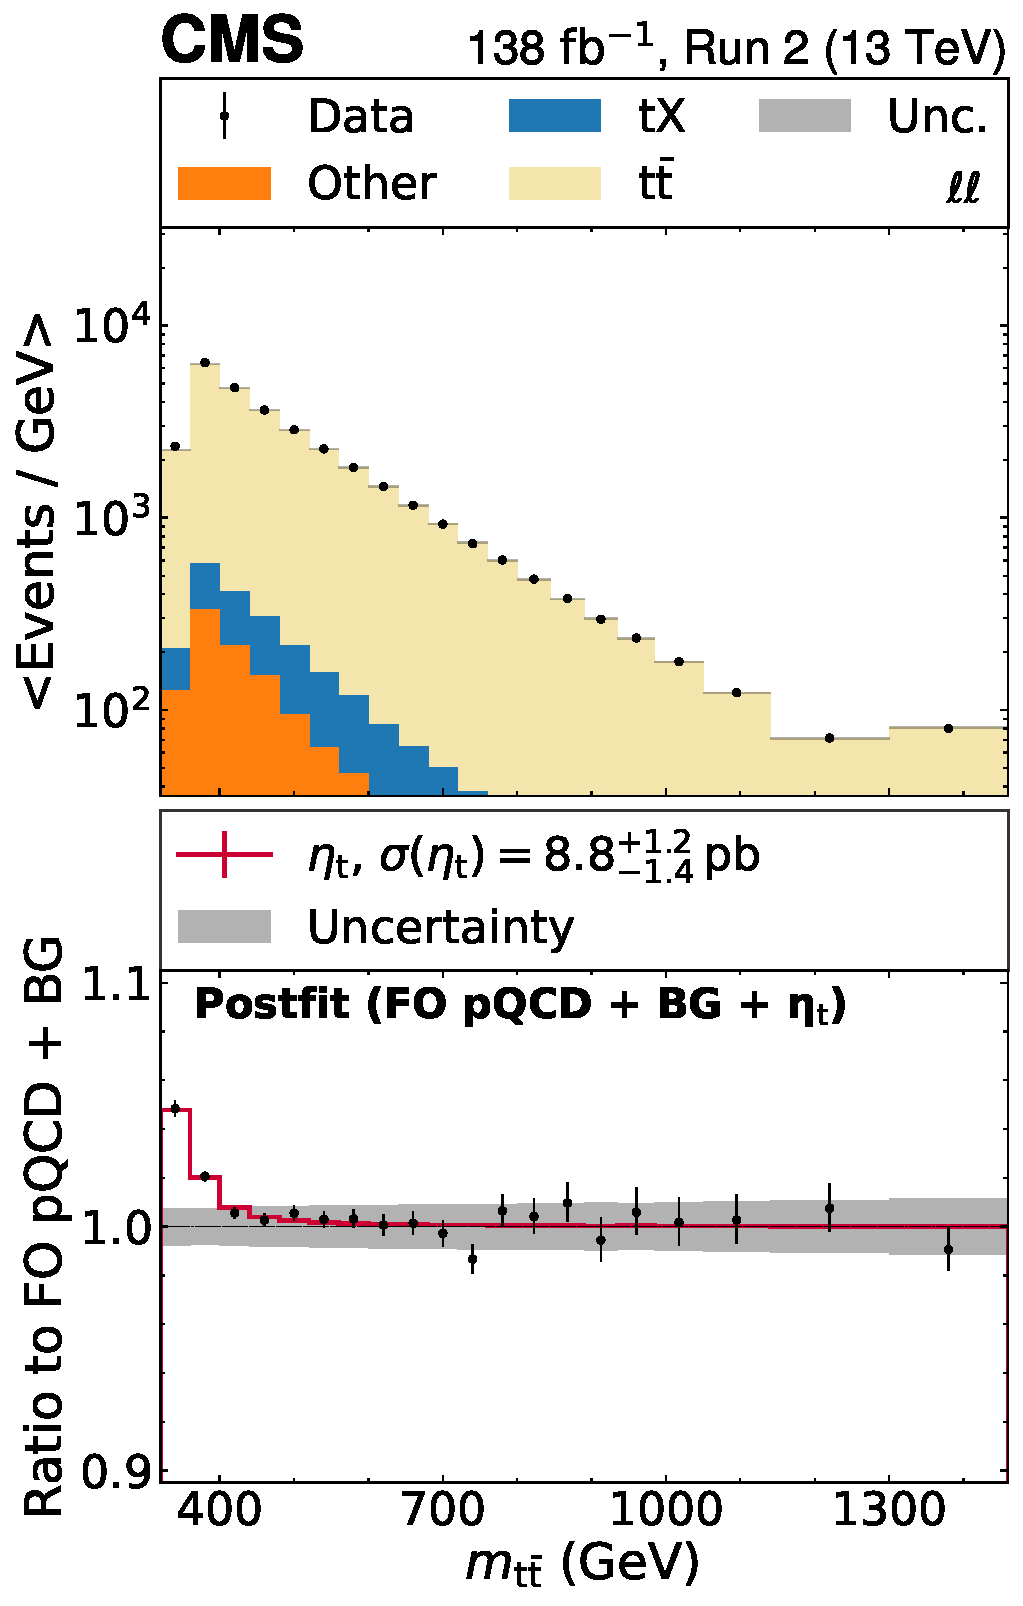
\includegraphics[width=0.32\textwidth]{figures/ah/prepost/EtaT_fit_s_ll_run2_both_mtt.pdf}
    \hfill
    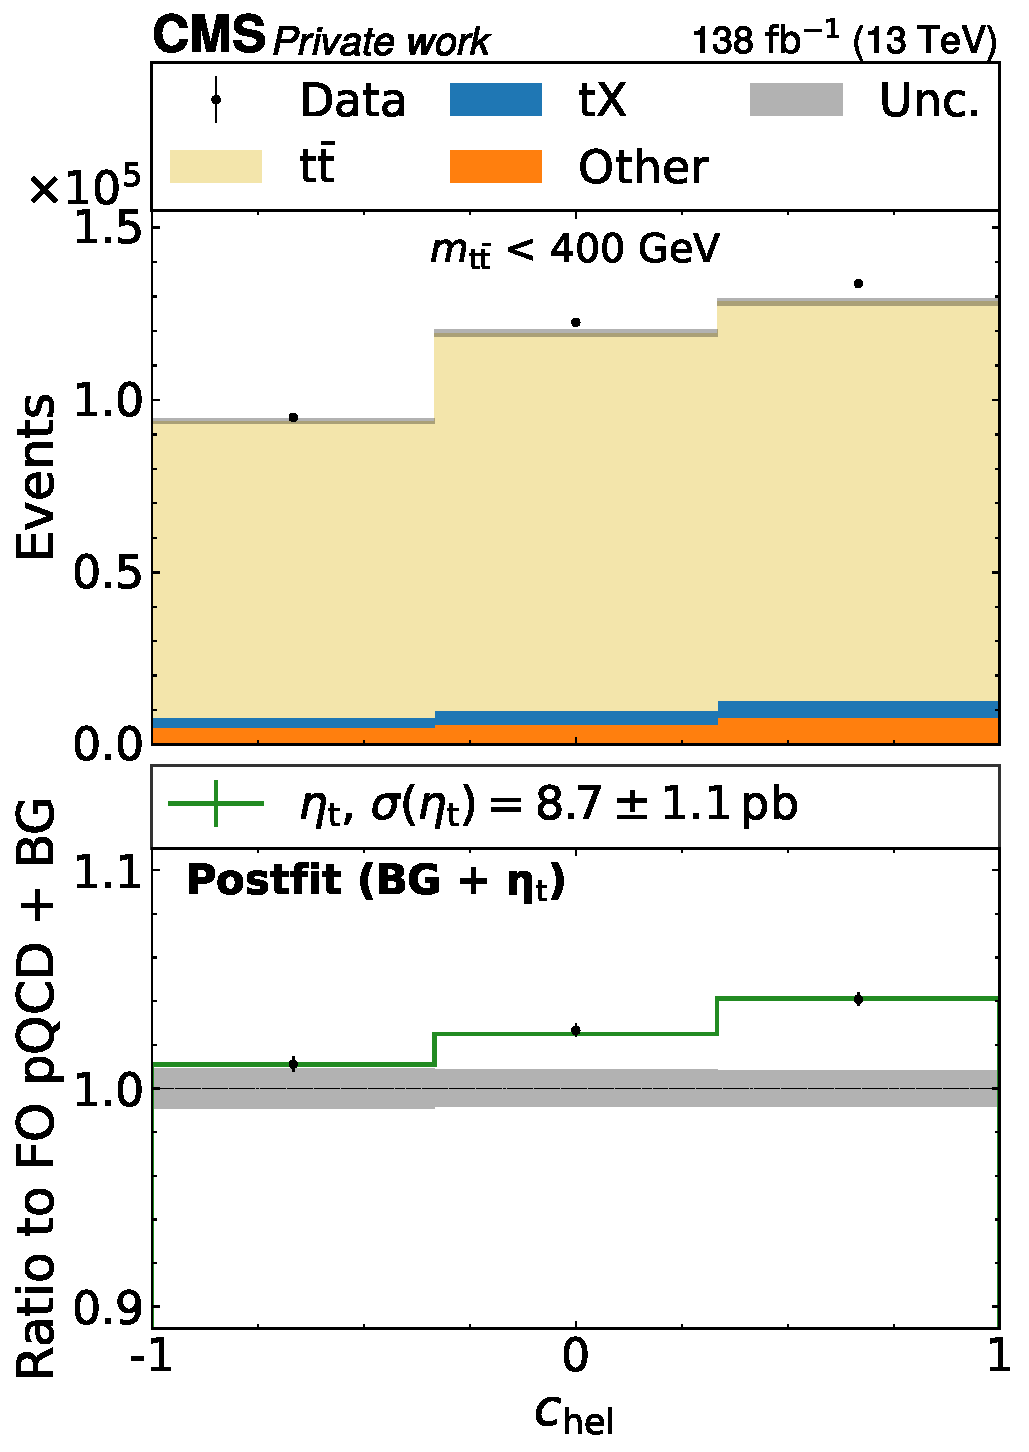
\includegraphics[width=0.32\textwidth]{figures/ah/prepost/EtaT_fit_s_ll_run2_both_chel_mttlt400.pdf}
    \hfill
    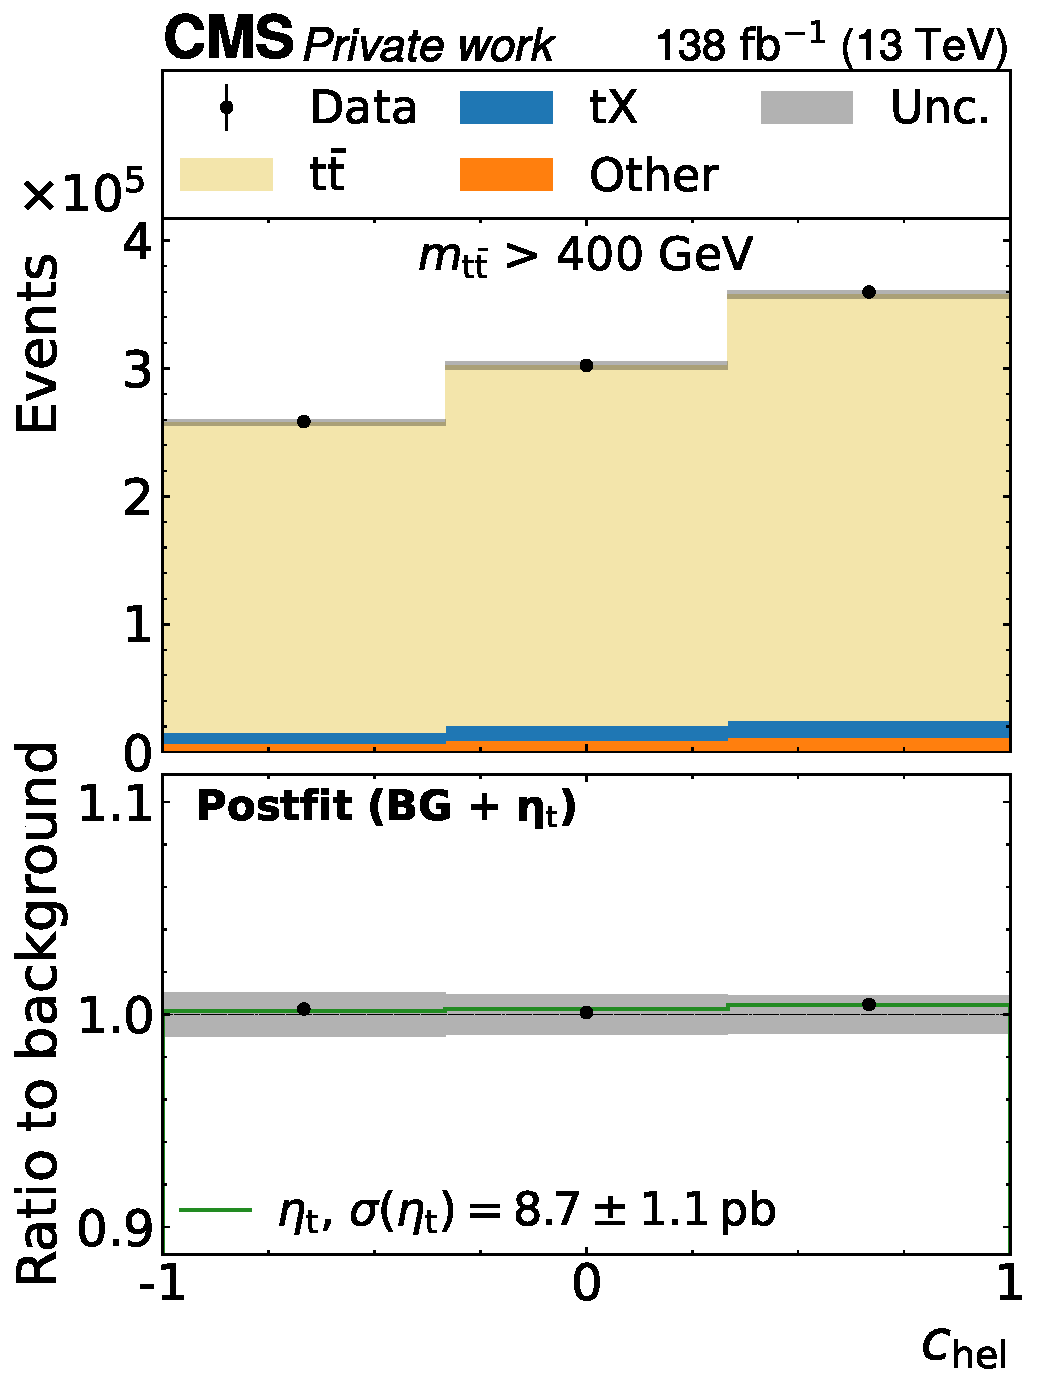
\includegraphics[width=0.32\textwidth]{figures/ah/prepost/EtaT_fit_s_ll_run2_both_chel_mttgt400.pdf}
    \caption{
        \label{fig:ah:postfit_etat_1d}
        \textbf{Postfit distributions of \mtt and \chel for the \etat fit.} One-dimensional distributions of inclusive \mtt (left), \chel for $\mtt < \SI{400}{\GeV}$ (center), and \chel for $\mtt > \SI{400}{\GeV}$ (right), projected from the \mttchelchan template in \cref{fig:ah:postfit_etat_ll} with the same notations. \textit{Figure adapted from \citere{CMS:TOP-24-007}}.
    }
    
\end{figure}

The postfit \mttchelchan distribution can be seen in \cref{fig:ah:postfit_etat_ll}. The data, including the excess at low \mtt, is described well by the \etat model combined with the FO pQCD background. To illustrate this further, one-dimensional projections of the \mttchelchan template into inclusive \mtt, as well as into \chel for both low and high \mtt, are shown in \cref{fig:ah:postfit_etat_1d}. One can clearly see that the data at the \ttbar threshold shows a stronger slope in data than in the FO pQCD prediction, consistent with the \etat signal, while no such slope is seen at high \mtt, i.e. in the \ttbar continuum.


\subsection{Parity of the excess}
\label{sec:ah:parityscan}

To investigate whether the observed excess is \CP-odd (pseudoscalar) or \CP-even (scalar) in nature, a simultaneous fit is performed with both \etat and \chit, as defined in \cref{sec:theory:etat}, as freely floating signals. These correspond to pure \term{1}{S}{0} and \term{3}{P}{0} \ttbar states, respectively, both localized at the \ttbar threshold.

\begin{figure}[th]
    \centering
    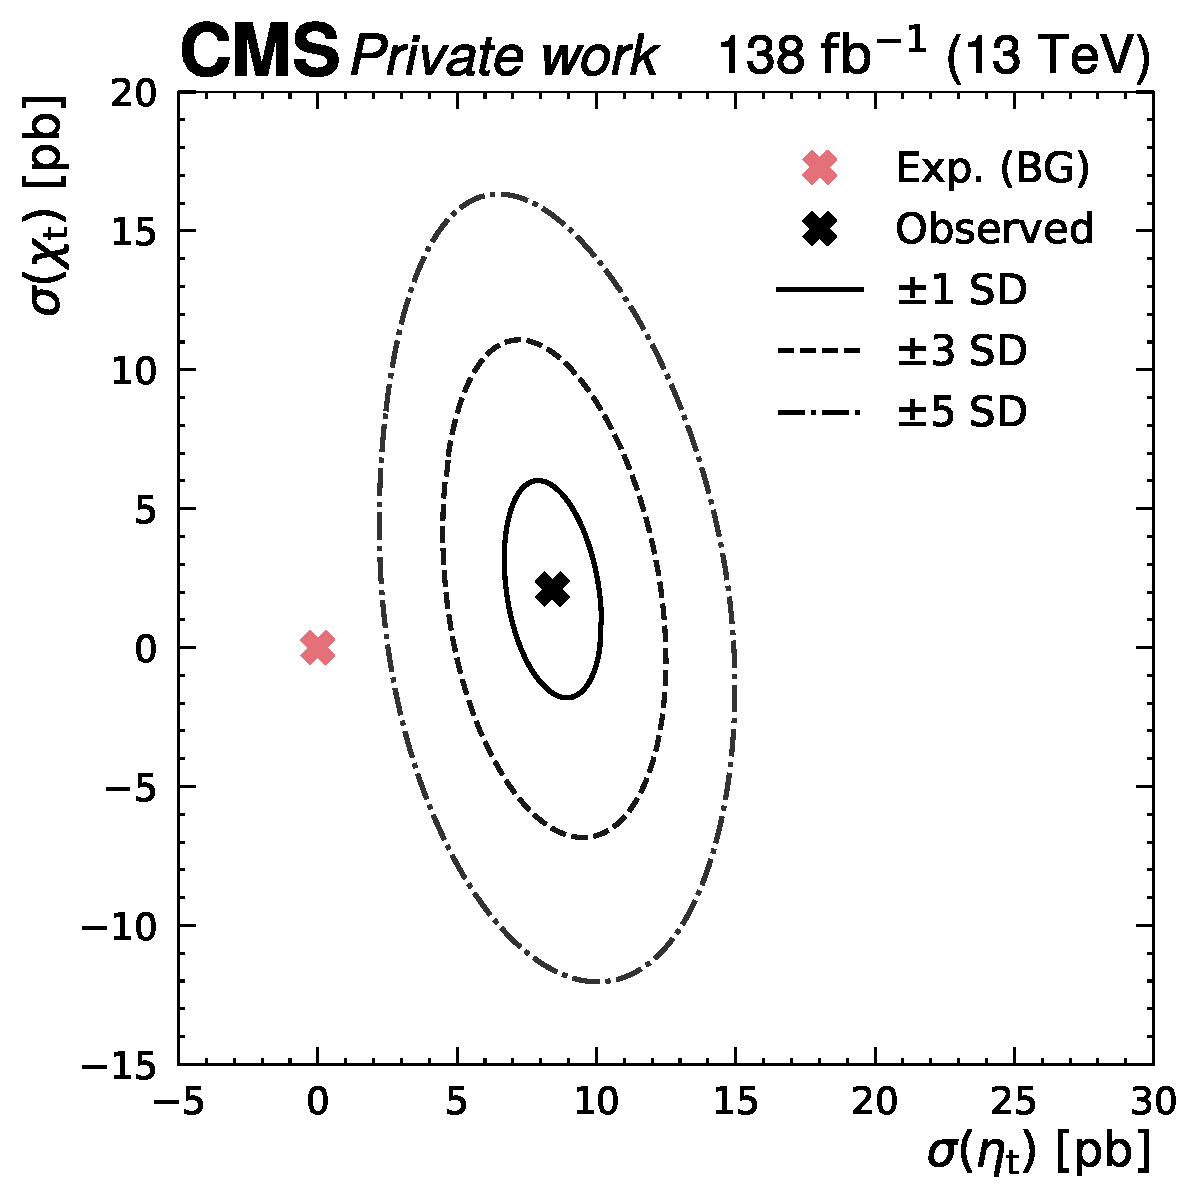
\includegraphics[width=0.6\textwidth]{figures/ah/etatfit/A_m365_w2p0__H_m365_w2p0_nll_CMS_EtaT_norm_13TeV__CMS_ChiT_norm_13TeV_ll.pdf}
    \caption{
        \textbf{Parity of the excess}. Observed compatibility contours in a simultaneous fit of \etat (corresponding to \term{1}{S}{0}) and \chit (corresponding to \term{3}{P}{0}). The best-fit point is shown as the black cross, while the BG-only expectation (i.e. $\sigetat=\sigma(\chit)=0$) is marked in pink. \textit{Figure adapted from \citere{CMS:TOP-24-007}}.
    }
    \label{fig:ah:parityscan}
\end{figure}

The result is shown in \cref{fig:ah:parityscan} in the form of compatibility contours. Consistent with the result of the \etat-only fit, a non-zero \etat contribution is preferred by the fit by more than 5 standard deviations. By contrast, the measured \chit cross section, which can be seen as the \term{3}{P}{0} component of the excess, is compatible with zero within one standard deviation. Based on this, it can be said that the observed excess is dominated by a pseudoscalar or \term{1}{S}{0} spin state.

\subsection{Checks of the result}
\label{sec:ah:checks}

\paragraph{Nuisance parameter pulls and impacts}

\begin{figure}[th]
    \centering
    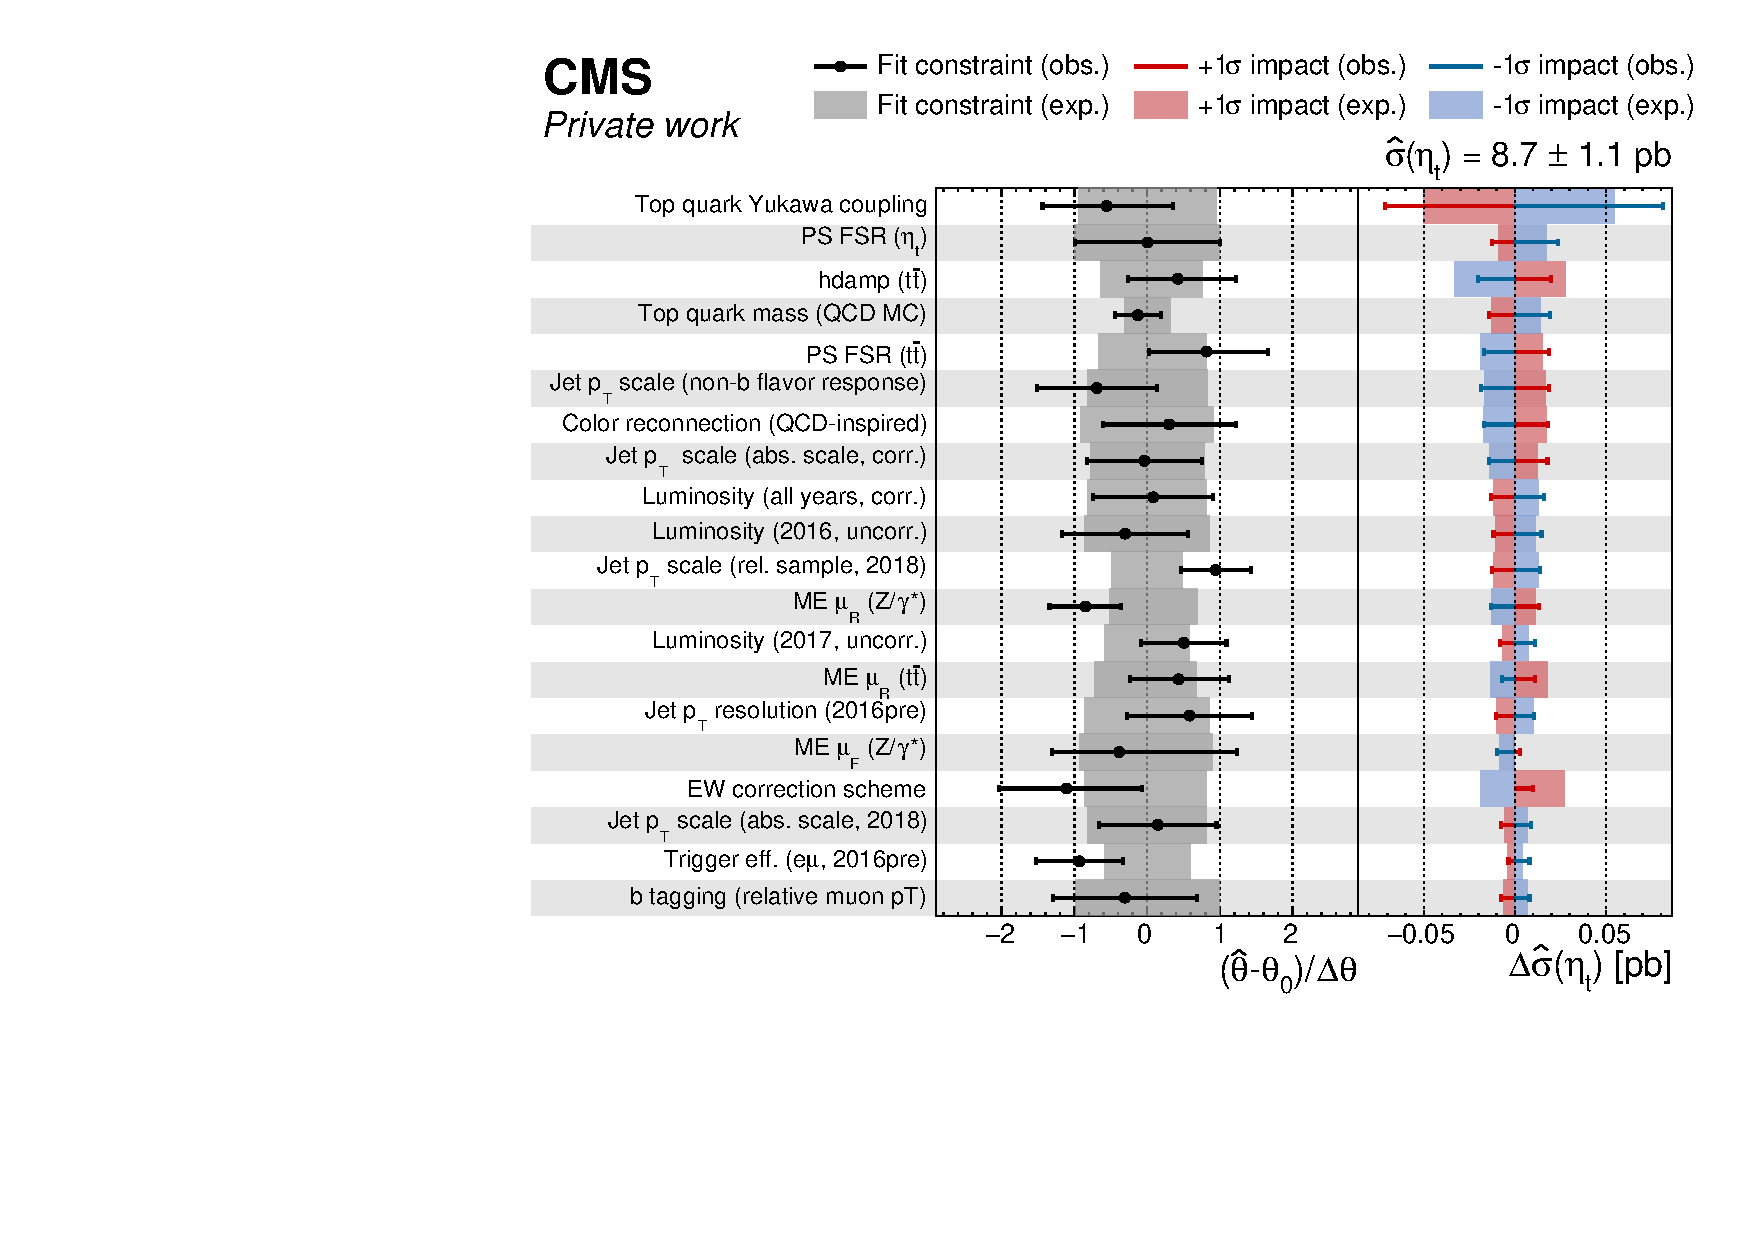
\includegraphics[width=0.9\textwidth]{figures/ah/etatfit/impacts_nonps.pdf}
    \caption{
        \textbf{Nuisance parameter pulls and impacts.} Expected and observed pulls, constraints, and impacts on the \etat cross section for the most impactful nuisance parameters in the \etat-only fit. \textit{Figure adapted from \citere{CMS:TOP-24-007}}.
    }
    \label{fig:ah:impacts_etat}
\end{figure}

In \cref{fig:ah:impacts_etat}, nuisance parameter pulls, constraints and impacts for the \etat extraction fit are presented, following the definitions in \cref{sec:methods:stat}. The most impactful nuisances are all related to the modeling of the \ttbar background. In particular, %the non-closure with respect to \bbfourl (cf. \cref{sec:ah:gennps}) and 
the value of the top Yukawa coupling \yt in the EW corrections is the leading uncertainty. This is notably one of the few uncertainties which can lead to a steeper \chel slope in the \ttbar prediction and could thus to some degree be confused for \etat, as discussed in \cref{sec:ah:ewcorr}. Further important modeling uncertainties are the FSR scales in the \ttbar parton shower as well as the top quark mass. 

On the other hand, experimental nuisances which influence mostly \mtt like the jet energy scales do not have a large impact on the POI. Regardless, no pulls larger than one prefit standard deviation are observed, indicating that the uncertainty model accommodates the data well.

\paragraph{Fit using \mbbll instead of \mtt}
The three observables \mtt, \chel and \chan are all obtained from the kinematic reconstruction as described in \cref{sec:ah:kinreco}. This procedure assumes, among others, that the top quarks are exactly on-shell with a fixed mass of \SI{172.5}{\GeV}. For \etat, which is located below the \ttbar threshold, this assumption is clearly violated. Since the same kinematic reconstruction procedure is applied to simulation and data, this is in principle not a problem as long as the virtuality of the top quarks is well described by simulation. However, since the modeling of \etat in particular is rather uncertain, it is still important to check whether this assumption in the kinematic reconstruction introduces any bias.

\begin{figure}[p]
    \centering
    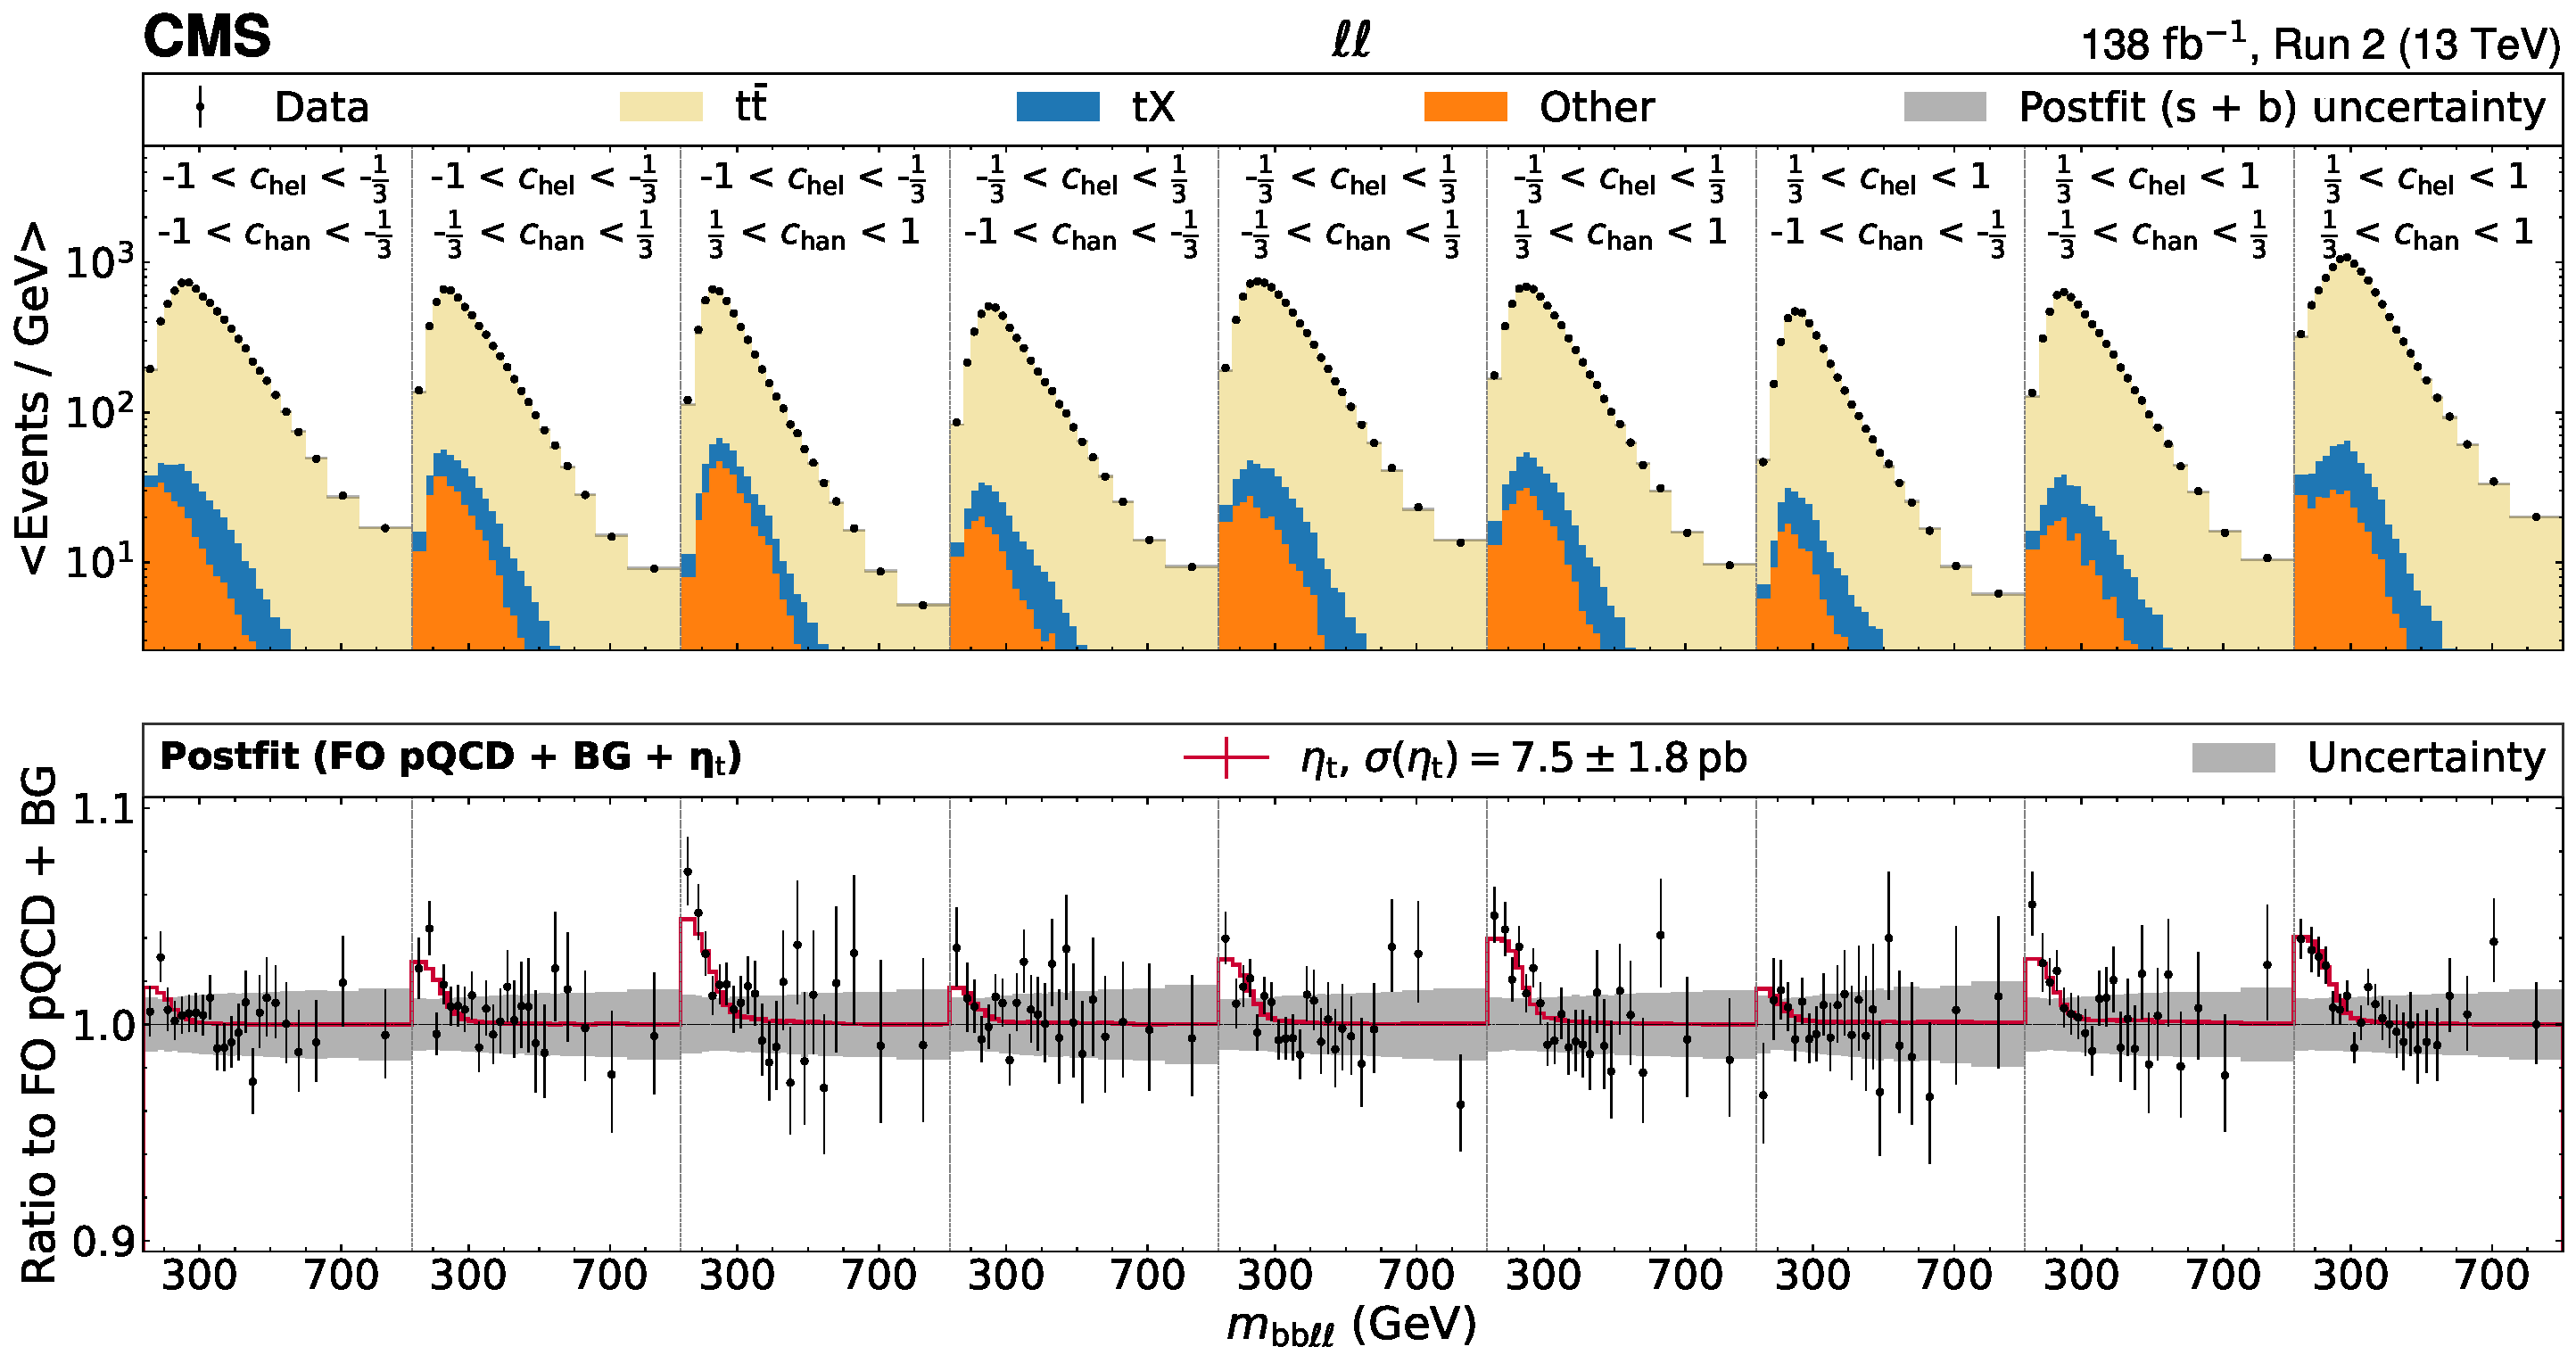
\includegraphics[width=0.99\textwidth]{figures/ah/prepost/EtaT_mbbllspin_fit_s_ll_run2_both.pdf}
    \caption{
        \label{fig:ah:postfit_mbbll_3D}
        \textbf{Postfit distributions of $\mbbll \times \chel \times \chan$ for the \etat fit.} The unrolled three-dimensional distribution in \mbbll, \chel and \chan after the fit to data with \etat as the signal using \mbbll instead of \mtt, summed over all years and lepton flavors. The first \mbbll bin in each $\chel \times \chan$ slice is an underflow bin containing events with $\mbbll < \SI{180}{\GeV}$. Otherwise, notations are as in \cref{fig:ah:postfit_etat_ll}.
    }
    \vspace{1cm}
    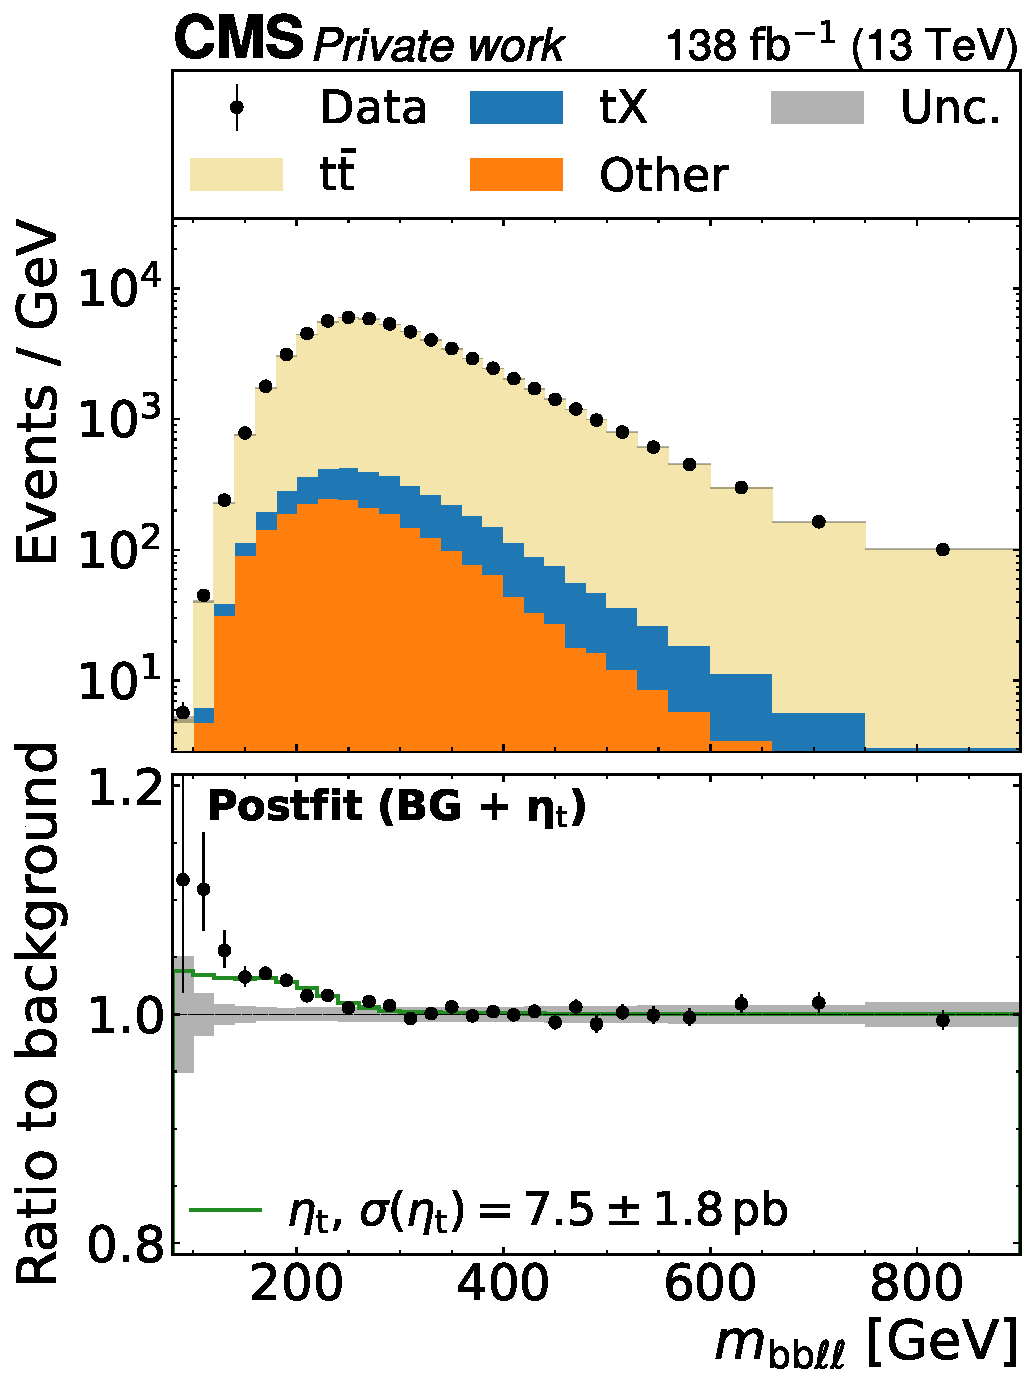
\includegraphics[width=0.32\textwidth]{figures/ah/prepost/EtaT_mbbllspin_fit_s_ll_run2_both_mbbll.pdf}
    \hfill
    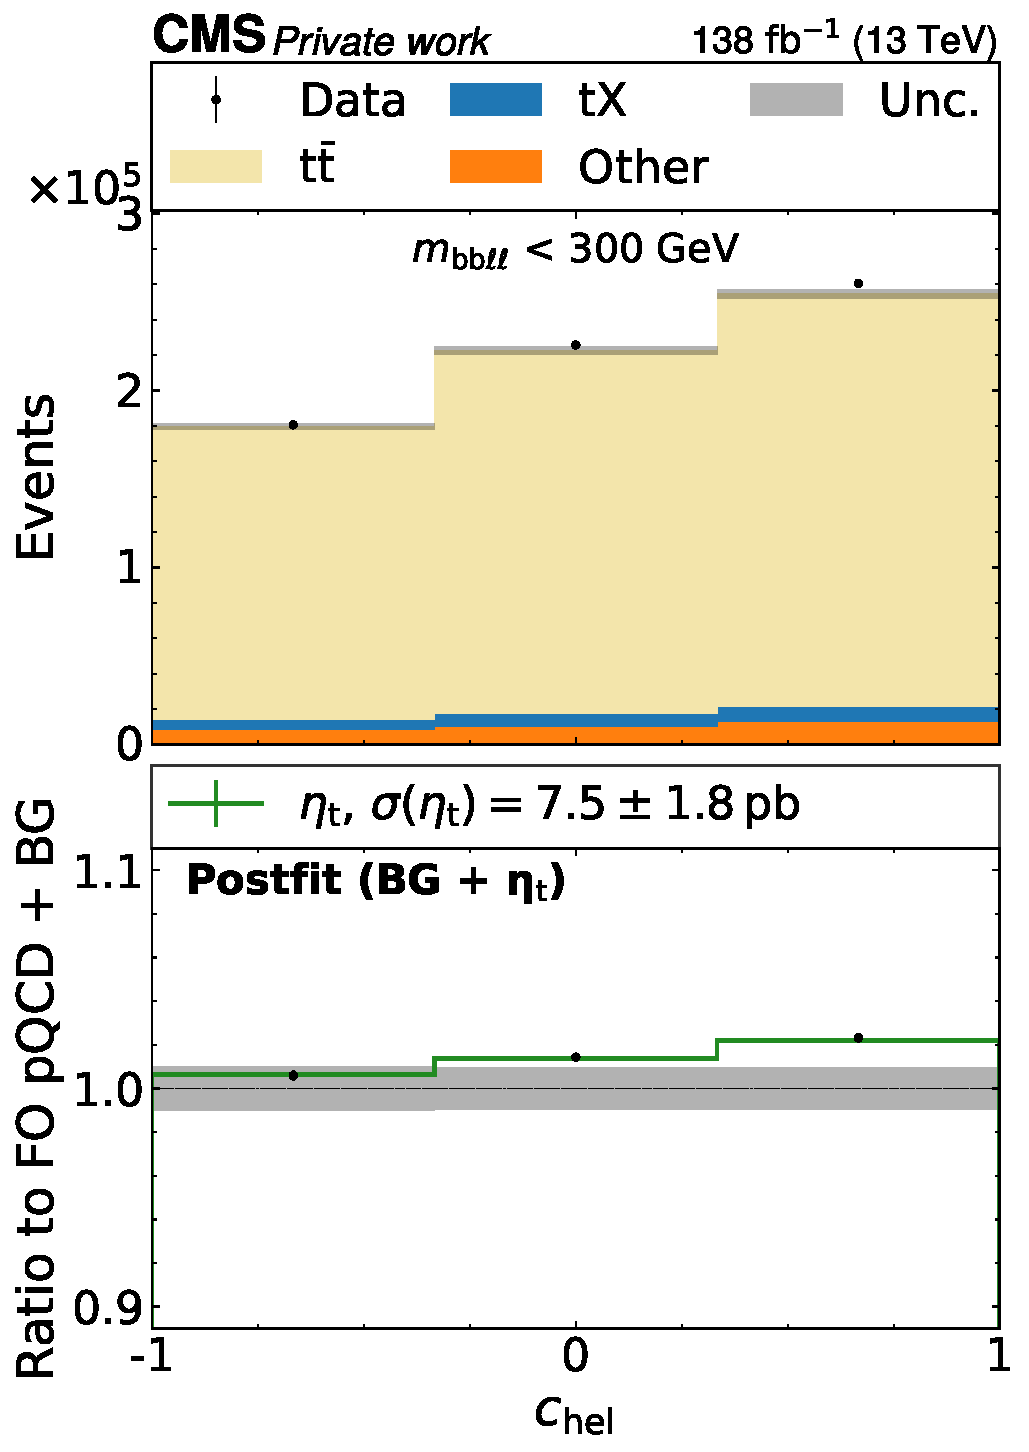
\includegraphics[width=0.32\textwidth]{figures/ah/prepost/EtaT_mbbllspin_fit_s_ll_run2_both_chel_mbblllt300.pdf}
    \hfill
    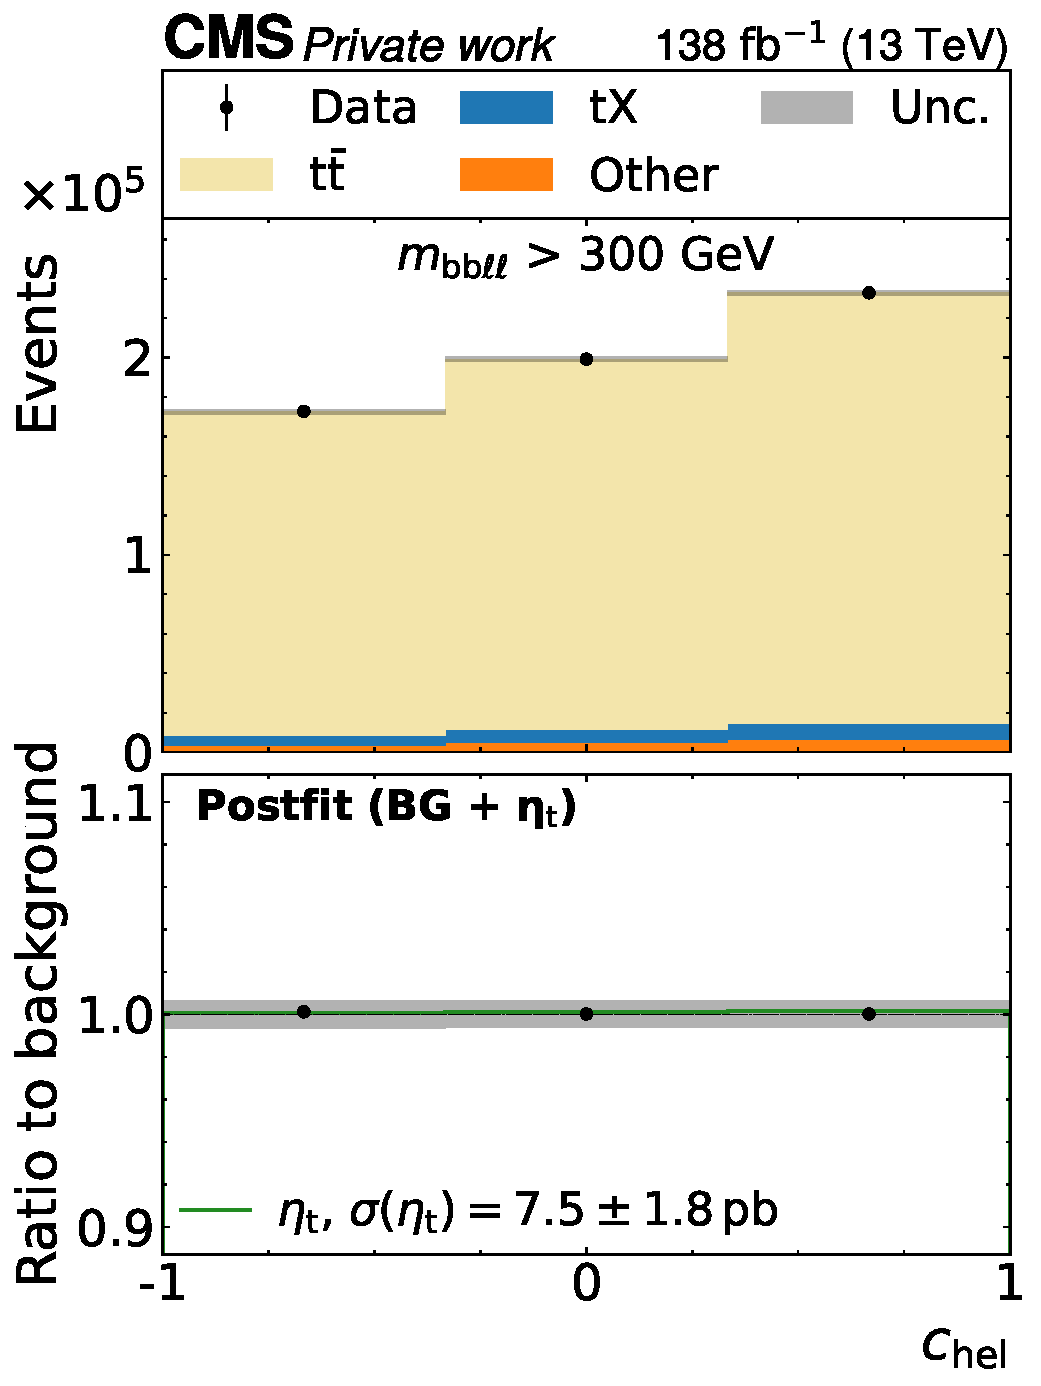
\includegraphics[width=0.32\textwidth]{figures/ah/prepost/EtaT_mbbllspin_fit_s_ll_run2_both_chel_mbbllgt300.pdf}
    \caption{
        \label{fig:ah:postfit_mbbll}
        \textbf{Postfit distributions of \mbbll and \chel for the \etat fit.} One-dimensional distributions of inclusive \mbbll (left), \chel for $\mbbll < \SI{300}{\GeV}$ (center), and \chel for $\mbbll > \SI{300}{\GeV}$ (right), projected from a 3D template of $\mbbll \times \chel \times \chan$. The first \mbbll bin in the left figure is an underflow bin containing events with $\mbbll < \SI{180}{\GeV}$. Otherwise, notations are as in \cref{fig:ah:postfit_etat_ll}. \textit{Figure adapted from \citere{CMS:TOP-24-007}}.
    }  
\end{figure}

%\begin{figure}[p]
%    \centering
%    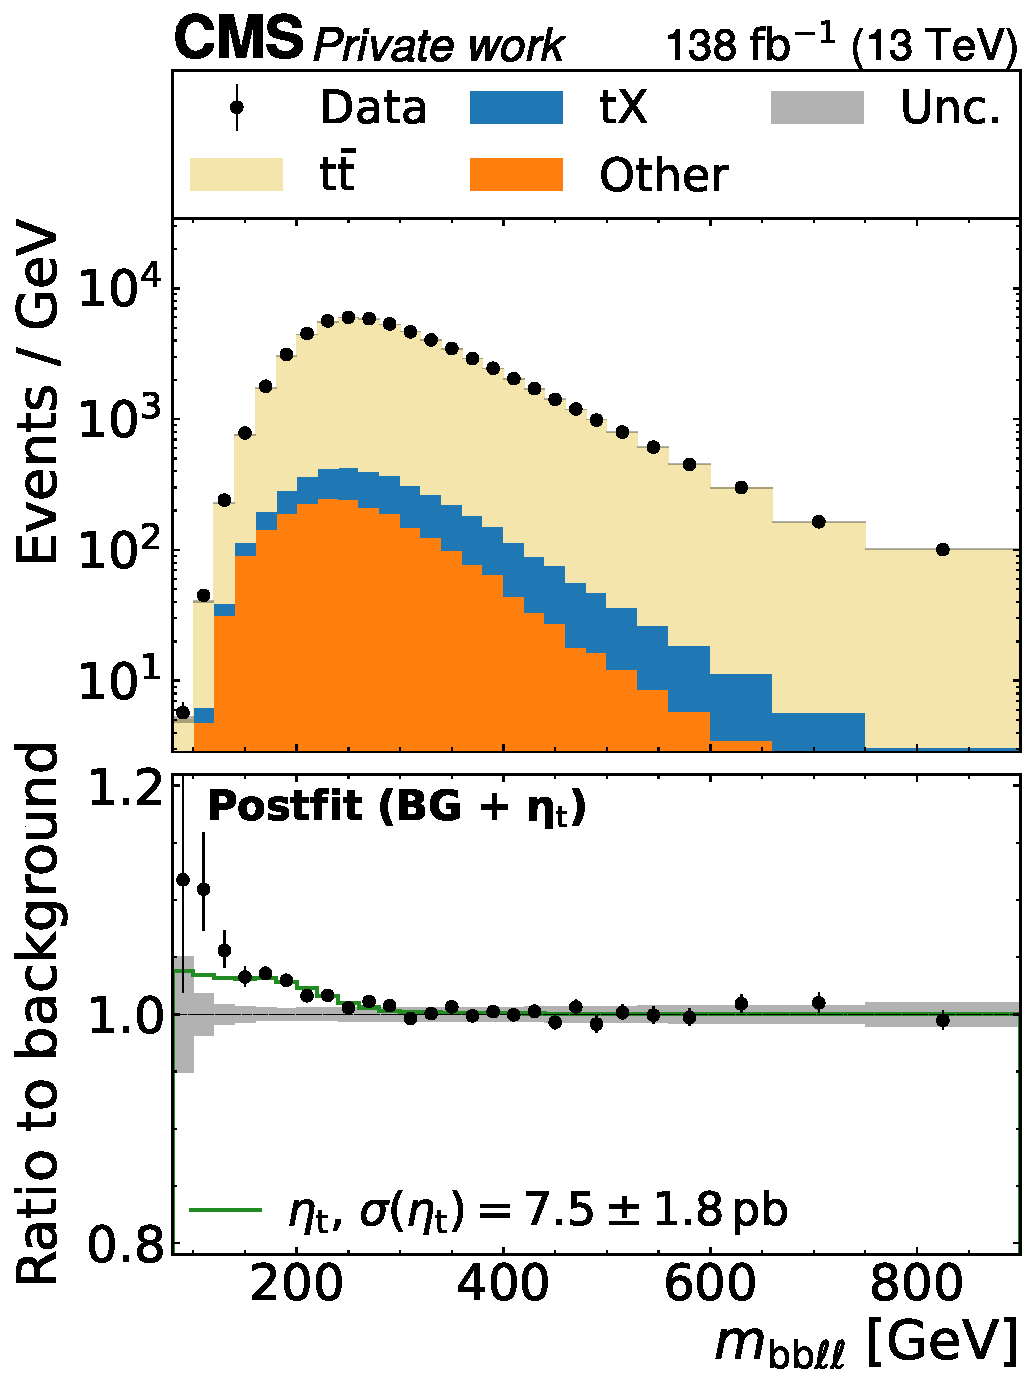
\includegraphics[width=0.32\textwidth]{figures/ah/prepost/EtaT_mbbllspin_fit_s_ll_run2_both_mbbll.pdf}
%    \hfill
%    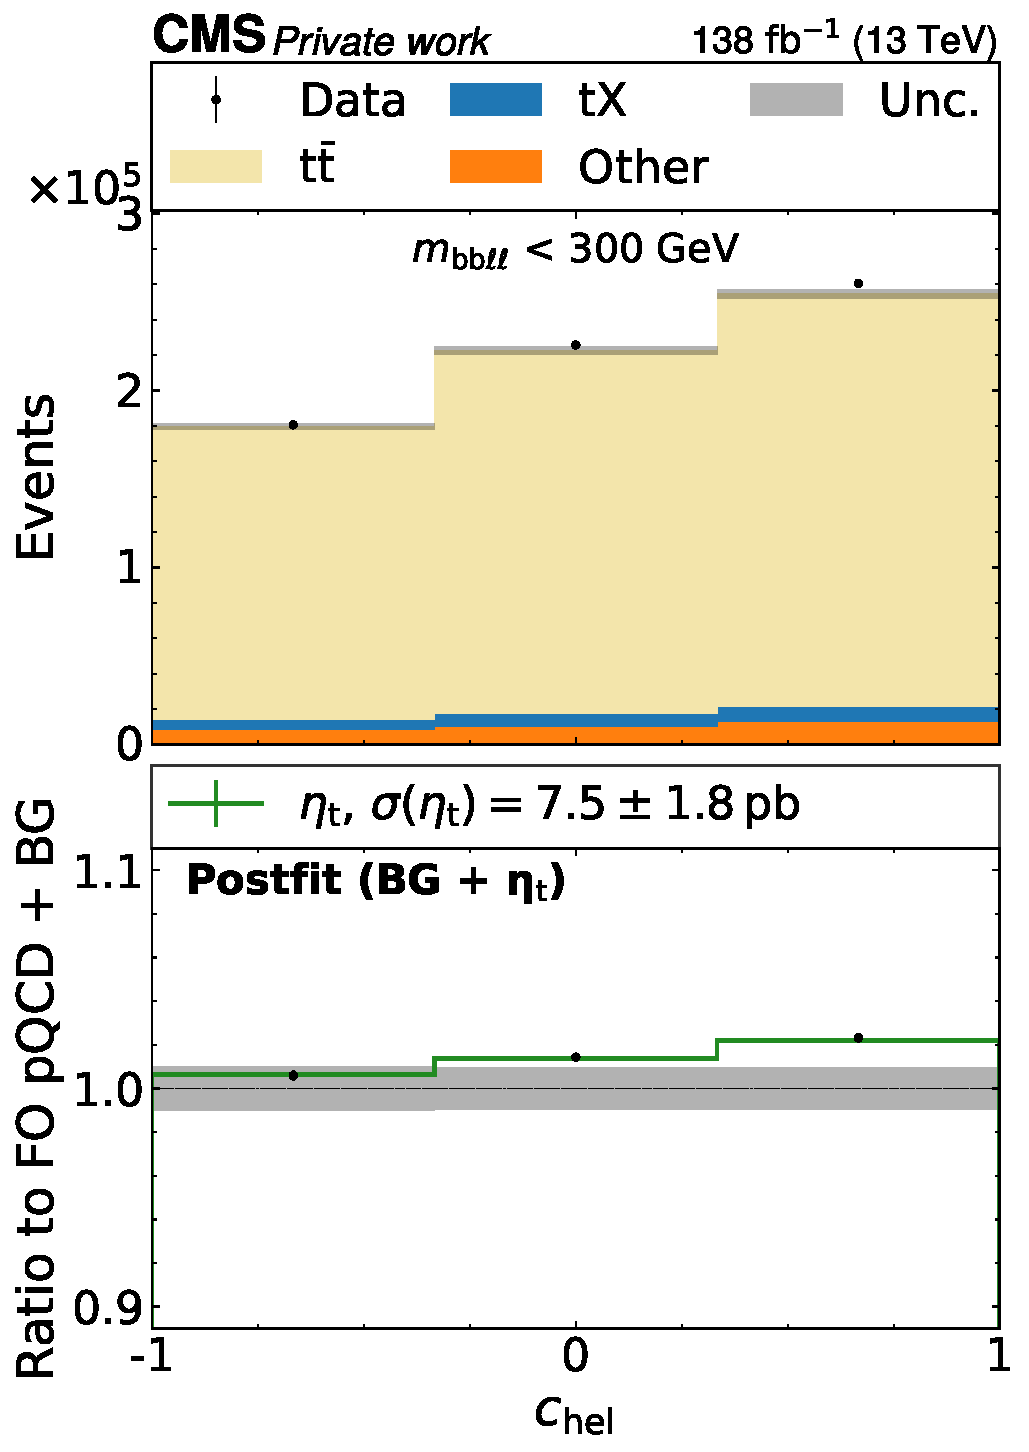
\includegraphics[width=0.32\textwidth]{figures/ah/prepost/EtaT_mbbllspin_fit_s_ll_run2_both_chel_mbblllt300.pdf}
%    \hfill
%    \includegraphics[width=0.32\textwidth]{figures/ah/prepost/EtaT_mbbllspin_fit_s_ll_run2_both_chel_mbbllgt300.pdf}
%    \caption{
%        \textbf{Postfit distributions of \mbbll and \chel for the \etat fit.} One-dimensional distributions of inclusive \mbbll (left), \chel for $\mbbll < \SI{300}{\GeV}$ (center), and \chel for $\mbbll > \SI{300}{\GeV}$ (right), projected from a 3D template of $\mbbll \times \chel \times \chan$. The first \mbbll bin in the left figure is an underflow bin containing events with $\mbbll < \SI{180}{\GeV}$. Otherwise, notations are as in \cref{fig:ah:postfit_etat_ll}.
%    }
%    \label{fig:ah:postfit_mbbll_1d}
%\end{figure}

This is done by repeating the fit with the observable \mtt replaced by \mbbll (as shown also in \cref{fig:ah:control3}), thus removing kinematic information obtained via the reconstruction from the fit. The kinematic reconstruction is still performed, however, to obtain \chel and \chan\footnote{It has separately been checked that the requirement for events to pass the kinematic reconstruction does not bias the result, either.}. %For this check, the nuisance parameters encoding the differences between generator setups (cf. \cref{sec:ah:gennps}) are not applied. 

The resulting $\mbbll \times \chel \times \chan$ postfit distribution can be found in \cref{fig:ah:postfit_mbbll_3D,fig:ah:postfit_mbbll}. It can be seen that the excess is still clearly present, though with a wider spread due to the coarser resolution of \mbbll compared to \mtt. An \etat cross section of $\sigetat = 7.5 \pm 1.8 \, \si{\pb}$ is extracted, which is in agreement with the nominal result within one standard deviation.

\paragraph{Alternate generator setups}

The influence of the choice of generator setup for the \ttbar prediction is further quantified by repeating the \etat extraction fit with alternate setups. Besides the nominal setup from \powheg \hvq matched to \pythia, the three setups introduced in \cref{sec:ah:gennps} are considered: \powheg \hvq matched to \herwig, \amcatnlo matched to \pythia with the FxFx scheme, and \bbfourl matched to \pythia. 
%The nuisance parameters encoding the non-closure with respect to these predictions are consequently not considered for this check. 
%Furthermore, a fourth alternative \ttbar prediction is considered, generated with \amcatnlo at NLO in QCD with up to one additional jet in the matrix element, and matched to \pythia using the FxFx merging scheme~\cite{Frederix:2012ps}

\begin{table}[th]
    \centering\renewcommand\arraystretch{1.1}
    \begin{tabular}{c|c}
    Generator setup & \sigetat [pb] \\
    \hline
    \hline
    \powheg \hvq + \pythia (nominal) & $8.7 \pm 1.1$ \\
    \powheg \hvq + \herwig & $8.6 \pm 1.1$ \\
    \amcatnlo FxFx + \pythia & $9.8 \pm 1.3$ \\
    \powheg \bbfourl + \pythia & $6.6 \pm 1.4$
\end{tabular}
\caption{%
    \textbf{Results for alternate generators.} Results for \sigetat obtained with different simulated event samples for the FO pQCD {\ttbar}+tW prediction.
    %Nuisance parameters encoding the difference between the generators were not included in these results.
}
\label{tab:ah:altbgs}
\end{table}

The results can be found in \cref{tab:ah:altbgs}. The results from \pythia and \herwig are fully in agreement with each other, while \amcatnlo results in a higher \etat cross section by about one standard deviation, and \bbfourl results in a lower \etat cross section by about $\sim 1.5$ standard deviations. 

As an additional check, the differences between the predictions from \powheg \hvq + \herwig and \powheg \hvq + \pythia as well as between \bbfourl and \tttWsum are included in the fit as additional nuisance parameters. In both cases, the \powheg \hvq + \pythia prediction is considered the nominal, and the alternate prediction is considered the $+1\sigma$ template. The $-1\sigma$ template is constructed by symmetrizing the relative difference around the nominal, and intermediate values are obtained by interpolation as usual.

\begin{figure}[!th]
    \centering
    \includegraphics[width=0.9\textwidth]{figures/ah/etatfit/impacts_gennps.pdf}
    \caption{
        \textbf{Nuisance parameter pulls and impacts including alternate generators.} Expected and observed pulls, constraints, and impacts on the \etat cross section for the most impactful nuisance parameters in the \etat-only fit where the differences between the predictions from \powheg \hvq + \herwig and \bbfourl + \pythia compared to \powheg \hvq + \pythia are included as additional nuisance parameters. \textit{Figure adapted from \citere{CMS:TOP-24-007}}.
    }
    \label{fig:ah:impacts_etat_gennps}
\end{figure}

The resulting \etat cross section with these nuisance parameters included is $\sigetat = 8.8^{+1.2}_{-1.4} \, \si{\pb}$\footnote{This figure is considered the nominal result in \citere{CMS:TOP-24-007}}. This figure is fully compatible with the nominal result with an asymmetrically increased uncertainty. The reason for the increase can be seen in \cref{fig:ah:impacts_etat_gennps}, showing the nuisance parameter pulls and impacts: The nuisance parameter encoding the difference between \bbfourl and \tttWsum represents the leading impact on the \etat cross section and is asymmetric. This is understandable from the steeper slope in \chel for \bbfourl as seen in \cref{fig:ah:herwigbb4l}, which is similar to the \etat signal, and is also in agreement with the reduced \etat cross section for a \bbfourl background prediction shown in \cref{tab:ah:altbgs}. It is furthermore significantly constrained towards zero, i.e. towards the default \tttWsum prediction, implying that the data prefers the NWA approach over the \textit{a priori} superior \bbfourl prediction. The reason for this is not readily apparent. One possible cause could be the fact that the NLO EW and NNLO QCD corrections are applied to \bbfourl in a necessarily ad-hoc manner, and might thus spoil the agreement with the data (cf. \cref{sec:ah:gennps}). However, in the scope of this work, this remains speculation.

On the other hand, the nuisance parameter encoding the difference of \pythia and \herwig is less impactful, consistent with the results for \herwig in \cref{tab:ah:altbgs}, and similarly strongly constrained. This is likely because the difference between \pythia and \herwig can be distinguished from \etat based on the combination of \mtt and \chel information, as expanded upon in \cref{sec:ah:gennps}.

\subsection{Interpretation in terms of A and H}
\label{sec:ah:bestfitah}

While a \ttbar bound state is the conceptually simplest explanation of the enhancement at the \ttbar threshold in the sense that it is predicted in the SM and does not invoke any further (BSM) degrees of freedom, it is also possible to perform an interpretation in terms of the generic spin-0 bosons A and H as introduced in \cref{sec:theory:ah}. 
For this purpose, fits allowing the presence of both A and H at the same time are performed. The two independent POIs are the A/H-top coupling modifiers \gAtt and \gHtt, and the interference with the SM is fully taken into account through a parameterization in terms of $\gAHtt^2$ and $\gAHtt^4$ (cf. \cref{eq:theory:ahxs}), thus allowing negative A/H contributions with respect to the SM.

A scan is performed over all pairs of considered A/H masses and widths (see \cref{sec:ah:datasets}), and the pair with the largest difference in logarithmic likelihood $\Delta \ln L$ is identified as the best-fit point. This results in $\mA = \SI{365}{\GeV}$, $\wA/\mA = 2\%$ for A and $\mH = \SI{925}{\GeV}$, $\wH/\mH = 3\%$ for H. It should be noted here that \SI{365}{\GeV} is the lowest mass point considered in the available signals for A and H, while \etat and \chit are located at a lower value of \SI{343}{\GeV}. It is possible that considering a lower value of \mA would lead to an even better fit; however, close to the \ttbar threshold, modeling the interference with the SM might be difficult due to large corrections at higher orders in QCD~\cite{Djouadi:2019,Djouadi:2024lyv}.

\begin{figure}[!th]
    \centering
    \includegraphics[width=0.99\textwidth]{figures/ah/prepost/A_m365_w2p0__H_m925_w3p0_fit_s_ll_run2_both.pdf}
    \caption{
        \textbf{Postfit distributions of \mttchelchan for the A+H fit.} The unrolled three-dimensional distribution in \mtt, \chel and \chan as after the fit to data with A and H as signals, summed over all years and lepton flavors. The A/H signals correspond to the best-fit masses and widths of $\mA = \SI{365}{\GeV}$, $\wA/\mA = 2\%$ for A and $\mH = \SI{925}{\GeV}$, $\wH/\mH = 3\%$ for H. The upper panel shows the sum of the background simulation (colored bars) and the observed data (black dots), while the lower panel shows the ratio of the data to the prediction with the postfit A and H signals, as well as their sum, overlaid.
    }
    \label{fig:ah:postfit_ah_ll}
\end{figure}

\begin{figure}[!th]
    \centering
    \includegraphics[width=0.6\textwidth]{figures/ah/contour/A_m365_w2p0__H_m925_w3p0_nll_g1__g2_ll_noetat.pdf}
    \caption{
        \textbf{Allowed coupling region in the A+H fit}. The two-dimensional allowed region for the coupling modifiers \gAtt and \gHtt in the A+H fit, for the best-fit A/H masses and widths of $\mA = \SI{365}{\GeV}$, $\wA/\mA = 2\%$ for A and $\mH = \SI{925}{\GeV}$, $\wH/\mH = 3\%$ for H, obtained through a scan of the profiled likelihood. The observed region is shown in black, while the SM expectation is shown in pink.
    }
    \label{fig:ah:contour_ah_ll}
\end{figure}

\Cref{fig:ah:postfit_ah_ll} shows the postfit \mttchelchan distribution, and \cref{fig:ah:contour_ah_ll} shows the allowed region for the two couplings \gAtt and \gHtt as obtained from a likelihood scan. From the latter, the best-fit values and total ranges for the coupling modifiers are found to be

\begin{equation}
\label{eq:ah:ahbestfit}
    \gAtt = 0.79^{+0.04}_{-0.05} \quad\quad \text{and} \quad\quad \gHtt = 1.47^{+0.17}_{-0.30}.
\end{equation}

The same excess close to the \ttbar threshold already seen in \cref{sec:ah:etat} manifests as of a non-zero value of \gAtt, which \cref{fig:ah:contour_ah_ll} shows is preferred by more than five standard deviations, similar as for the interpretation in terms of \etat. In addition, there is also a preference for a non-zero value of \gHtt, though this is significant only at about 2 standard deviations and could thus be a simple statistical fluctuation. It should be noted that both of these values are local significances, i.e. they do not account for the look-elsewhere effect. The source of this preference is again evident from \cref{fig:ah:postfit_ah_ll}: it is due to a mild, broad excess in events compared to the prediction around $\mtt \approx \SI{900}{\GeV}$, which is more pronounced in the low \chan bins compared to the others as would be expected for a scalar particle H.

It is important to stress that these results do not constitute any observation of a new BSM particle. Given the experimental resolution in \mtt, as well as the signal mass points available, the \ttbar bound state \etat and a BSM pseudoscalar A cannot be conclusively distinguished. 

% what to do with the GEN NPs

% plan:
% do best fits for A, H, EtaT. show in table: best fit POI + unc, p value
% for A,H this means scan over masses/ widths. hopefully it comes out to be small
% postfit plots for both
% then: stat checks. impacts, GOF (for etat only probably)
% possibly table with tests. bb4l, herwig, mbbllspin. TBD, see what ends up in the paper
% discussion. problems with the model. experimentally sound. modeling uncertain.
% 

%The prefit excess visible in \cref{fig:ah:prefit_ll} is interpreted by performing signal+background fits for three different signals: A, H, and the parametrized \ttbar bound state model \etat. For A and H, the coupling strength modifiers \gAtt and \gHtt are used as parameters of interest (POI), and both resonance and interference are considered, scaling with the fourth and second power of the POI, respectively. For \etat, where there is no such scaling, the cross section of the \etat signal is considered as the measured quantity, and a linear signal strength $\muetat = \sigetat / \sigetatpred$ is defined as the POI. A value of $\sigetatpred = \SI{6.43}{\pb}$~\cite{Fuks:2021xje} is used for the normalization; this value is used only for display purposes and does not influence the fit results in any way.

\section{Limits on A/H bosons}
\label{sec:ah:limits}

Having discussed the excess seen at the \ttbar threshold and its possible interpretations, in this section exclusion limits on \AH bosons in the full considered mass range are presented. This is done for two different scenarios: In the first scenario, denoted ``A/H only'', the SM \ttbar background is described by the FO pQCD prediction from \powheg + \pythia reweighted to NLO EW and NNLO QCD, same as for the \etat extraction in \cref{sec:ah:etat} and for the A+H fit in \cref{sec:ah:bestfitah}. The observed excess is thus expected to manifest in the limits in the form of a weaker observed than expected limit for low A/H masses.

In the second scenario, denoted ``A/H + \etat'', the observed excess is assumed to originate solely from a \ttbar bound state, which is further assumed to be well described by the \etat model. Under this assumption, the \etat contribution is added to the \ttbar background prediction, with a free-floating normalization as an additional nuisance parameter. A and/or H contributions are then considered as signals on top of this background. It should be stressed that, while \cref{fig:ah:postfit_etat_ll} shows good agreement of the \etat description with the data, the true cause of the excess cannot be fully determined with the available \mtt resolution. Thus, all limits shown here should be treated with caution for low values of the \AH mass.

In both scenarios, the limits are calculated with the \CLs prescription as introduced in \cref{sec:methods:stat}. However, a complication is presented by the non-linearity of the A/H signal as a function of \gAHtt, due to which the distribution of the test statistic is not necessarily $\chi^2$-distributed, and thus the $p$-values $p_{\mathrm{s+b}}$ and $p_{\mathrm{b}}$ cannot be easily computed. To avoid having to perform computationally expensive toy experiments, a \textit{raster scan} method is used in the same way as in \citere{CMS:HIG-17-027}. For a given \AH mass and width point, the coupling modifier \gAHtt is scanned in the range 0--5. For each value of \gAHtt, the total signal contribution is computed as the sum of the resonant signal, scaling with $\gAHtt^4$, and the SM-signal interference, scaling with $\gAHtt^2$. An auxiliary linear signal strength $\mu$ is then introduced, so that the total signal contribution becomes

\begin{equation}
    s (\mu) = \mu \left( \gAHtt^4 \, s_{\mathrm{res}} + \gAHtt^2 \, s_{\mathrm{int}} \right)
\end{equation}

\noindent where $s_{\mathrm{res}}$ and $s_{\mathrm{int}}$ are the resonance and interference contributions, respectively, and \gAHtt is held fixed. $\mu = 1$ corresponds to the probed A/H signal, while $\mu = 0$ corresponds to the SM. Intermediate values of $\mu$ are in principle unphysical since they do not correspond to any value of \gAHtt.

Since the A/H signal now scales linearly with $\mu$, the usual asymptotic approximation can be used to obtain the \CLs value for $\mu = 1$. It has been shown as a part of \citere{CMS:HIG-17-027} that the distribution of the test statistic obtained in this way approximates well the true test statistic for \gAHtt as evaluated using toy experiments. This procedure is repeated for all values of \gAHtt, and a value of \gAHtt is, as usual, excluded at 95\% confidence level when the \CLs value drops below 0.05. 

The resulting observed and expected limits for all considered A and H masses and six representative width choices are shown in \cref{fig:ah:limit_1D_a_smtt,fig:ah:limit_1D_h_smtt} for the ``A/H only'' scenario and in \cref{fig:ah:limit_1D_a_etat,fig:ah:limit_1D_h_etat} for the ``A/H + \etat'' scenario. In the ``A/H only'' scenario, the excess at the \ttbar threshold is visible at low A/H masses as expected. It is stronger for the pseudoscalar A than for the scalar H, consistent with the results in \cref{sec:ah:parityscan}. In the ``A/H + \etat'' scenario, the excess is fully absorbed by the \etat contribution, and the observed and expected limits at low A/H masses agree. It is notable here that the expected limits change only little between the scenarios even though, in the ``A/H + \etat'' scenario, the cross section of the \etat contribution is freely floating in the fit. \todo{decide on whether I want to elaborate on this, would need a plot of the signal templates}

Furthermore, the mild excess for H at high masses as seen in \cref{fig:ah:contour_ah_ll} is reproduced in the limits on \gHtt in both scenarios in the approximate range of $900 < \mH < \SI{1000}{\GeV}$.

\begin{figure}[!ph]
    \centering
    \includegraphics[width=0.42\textwidth]{figures/ah/lim1D/smtt/ll/A_limit_w1p0_g-scan.pdf}%
    \hspace*{0.05\textwidth}%
    \includegraphics[width=0.42\textwidth]{figures/ah/lim1D/smtt/ll/A_limit_w2p0_g-scan.pdf} \\
    \includegraphics[width=0.42\textwidth]{figures/ah/lim1D/smtt/ll/A_limit_w5p0_g-scan.pdf}%
    \hspace*{0.05\textwidth}%
    \includegraphics[width=0.42\textwidth]{figures/ah/lim1D/smtt/ll/A_limit_w10p0_g-scan.pdf}
    \\
    \includegraphics[width=0.42\textwidth]{figures/ah/lim1D/smtt/ll/A_limit_w18p0_g-scan.pdf}%
    \hspace*{0.05\textwidth}%
    \includegraphics[width=0.42\textwidth]{figures/ah/lim1D/smtt/ll/A_limit_w25p0_g-scan.pdf}
    \caption{%
        \textbf{Exclusion limits on \gAtt in the ``A only'' scenario} in the dilepton channels as a function of the mass of the A boson  for relative widths of 1, 2, 5, 10, 18, and 25\% (from upper left to lower right).
        The observed limits are indicated by the blue shaded area, and the inner green band and the outer yellow band indicate the regions containing 68 and 95\%, respectively, of the distribution of limits expected under the background-only hypothesis.
        The unphysical region of phase space in which the partial width $\Gamma_{\mathrm{A \rightarrow \ttbar}}$ becomes larger than the total width of A is indicated by the hatched line.
    }
    \label{fig:ah:limit_1D_a_smtt}
\end{figure}
    
\begin{figure}[!ph]
    \centering
    \includegraphics[width=0.42\textwidth]{figures/ah/lim1D/smtt/ll/H_limit_w1p0_g-scan.pdf}%
    \hspace*{0.05\textwidth}%
    \includegraphics[width=0.42\textwidth]{figures/ah/lim1D/smtt/ll/H_limit_w2p0_g-scan.pdf} \\
    \includegraphics[width=0.42\textwidth]{figures/ah/lim1D/smtt/ll/H_limit_w5p0_g-scan.pdf}%
    \hspace*{0.05\textwidth}%
    \includegraphics[width=0.42\textwidth]{figures/ah/lim1D/smtt/ll/H_limit_w10p0_g-scan.pdf}
    \\
    \includegraphics[width=0.42\textwidth]{figures/ah/lim1D/smtt/ll/H_limit_w18p0_g-scan.pdf}%
    \hspace*{0.05\textwidth}%
    \includegraphics[width=0.42\textwidth]{figures/ah/lim1D/smtt/ll/H_limit_w25p0_g-scan.pdf}
    \caption{%
        \textbf{Exclusion limits on \gHtt in the ``H only'' scenario} in the dilepton channels as a function of the mass of the H boson. Notations are equivalent to \cref{fig:ah:limit_1D_a_smtt}.
    }
    \label{fig:ah:limit_1D_h_smtt}
\end{figure}

\begin{figure}[!ph]
    \centering
    \includegraphics[width=0.42\textwidth]{figures/ah/limits_etat_w2p8/A_limit_w1p0_g-scan.pdf}%
    \hspace*{0.05\textwidth}%
    \includegraphics[width=0.42\textwidth]{figures/ah/limits_etat_w2p8/A_limit_w2p0_g-scan.pdf} \\
    \includegraphics[width=0.42\textwidth]{figures/ah/limits_etat_w2p8/A_limit_w5p0_g-scan.pdf}%
    \hspace*{0.05\textwidth}%
    \includegraphics[width=0.42\textwidth]{figures/ah/limits_etat_w2p8/A_limit_w10p0_g-scan.pdf}
    \\
    \includegraphics[width=0.42\textwidth]{figures/ah/limits_etat_w2p8/A_limit_w18p0_g-scan.pdf}%
    \hspace*{0.05\textwidth}%
    \includegraphics[width=0.42\textwidth]{figures/ah/limits_etat_w2p8/A_limit_w25p0_g-scan.pdf}
    \caption{%
        \textbf{Exclusion limits on \gAtt in the ``A + \etat'' scenario} in the dilepton channels as a function of the mass of the A boson. Notations are equivalent to \cref{fig:ah:limit_1D_a_smtt}.
    }
    \label{fig:ah:limit_1D_a_etat}
\end{figure}
    
\begin{figure}[!ph]
    \centering
    \includegraphics[width=0.42\textwidth]{figures/ah/limits_etat_w2p8/H_limit_w1p0_g-scan.pdf}%
    \hspace*{0.05\textwidth}%
    \includegraphics[width=0.42\textwidth]{figures/ah/limits_etat_w2p8/H_limit_w2p0_g-scan.pdf} \\
    \includegraphics[width=0.42\textwidth]{figures/ah/limits_etat_w2p8/H_limit_w5p0_g-scan.pdf}%
    \hspace*{0.05\textwidth}%
    \includegraphics[width=0.42\textwidth]{figures/ah/limits_etat_w2p8/H_limit_w10p0_g-scan.pdf}
    \\
    \includegraphics[width=0.42\textwidth]{figures/ah/limits_etat_w2p8/H_limit_w18p0_g-scan.pdf}%
    \hspace*{0.05\textwidth}%
    \includegraphics[width=0.42\textwidth]{figures/ah/limits_etat_w2p8/H_limit_w25p0_g-scan.pdf}
    \caption{%
        \textbf{Exclusion limits on \gHtt in the ``H + \etat'' scenario} in the dilepton channels as a function of the mass of the H boson. Notations are equivalent to \cref{fig:ah:limit_1D_a_smtt}.
    }
    \label{fig:ah:limit_1D_h_etat}
\end{figure}

\section{Combination with the \texorpdfstring{\ljets}{l+jets} channels}
\label{sec:ah:combination}

So far, all results in this section have covered only the dilepton decay channel of \ttbar, which was analyzed as part of this thesis. In \citere{CMS:HIG-22-013-PAS}, the results on A/H bosons are combined with a separate analysis of the \ljets decay channel. The combination (but not the \ljets analysis) was also performed as part of this thesis, and is presented in this chapter. The \ljets analysis strategy is roughly outlined in the following, for a more complete description, see \citere{CMS:HIG-22-013-PAS}.

\subsection{Analysis strategy in the \texorpdfstring{\ljets}{l+jets} channel}
\label{sec:ah:ljets}

In the \ljets channel, events with exactly one lepton and at least three jets are selected, of which at least two need to be b tagged. In addition to the criteria outlined in \cref{sec:ah:objects}, both the lepton and the jets are required to fulfill $\pt > \SI{30}{\GeV}$ to account for the higher single-lepton trigger thresholds. Furthermore, the cut-based identification criteria for electrons, as described in \citere{CMS:EGM-17-001}, are applied instead of MVA-based criteria. Similar as in the dilepton channel, the events are categorized by the flavor of the lepton into the \ejets and \mujets channels.

The algorithm described in \citere{Betchart:2013nba} is used to reconstruct the neutrino from the leptonic top decay. It enforces mass constraints on the W boson and leptonically decaying top quark and then minimizes the distance $D_\nu = |\pt^\nu - \ptmiss|$ between the neutrino \pt and the missing transverse momentum. In events with four or more jets, the same distance $D_\nu$ is then also used to assign the jets to the b and $\bar{\mathrm{b}}$ candidates as well as to the decay products of the hadronically decaying W boson. From this, the \ttbar system can then be reconstructed. In events with exactly three jets, where information has been lost due to either an out-of-acceptance jet or the merger of two jets into one, additional steps have to be taken. The procedure described in \citere{Demina:2013wda} is applied to these events, which involves applying an energy correction factor to the four-momentum of the hadronically decaying top quark, depending on its reconstructed mass. Since the resolution of this procedure is necessarily worse than for events where all jets are available, events with three jets and four or more jets are treated as separate categories in the fit.

A two-dimensional template is constructed from the reconstructed value of \mtt as well as \abscostl, where $\theta^*_\ell$ is the scattering angle of the leptonically decaying top quark with respect to the direction of flight of the \ttbar system in the laboratory frame. This variable is sensitive to the spin of a possible mediator in \ttbar production: For spin-0 mediators like \AH, the top quarks are emitted isotropically in the \ttbar rest frame, leading to a flat distribution of \abscostl, while in the SM \abscostl peaks at high values. However, it is not sensitive to the \CP structure of the mediator, in contrast to \chel and \chan. Furthermore, the SM prediction changes as a function of \mtt; close to the \ttbar threshold, the difference to a flat spectrum is rather small, while for high \mtt the difference is large due to the impact of the $q\bar{q}$ initial state. 

The \ttbar and tW background predictions as well as the A/H signals are estimated using the same MC simulation as in the dilepton channels. Additionally, there is a significant background contribution from QCD multijet production with a fake or non-prompt lepton as well as EW processes such as W+jets production. These are difficult to model using MC, and are instead estimated together by a data-driven approach (cf. \cref{sec:ttxs:datadriven}). A sideband in which the b tagging requirement on the jets is inverted is used for this purpose; details can be found in \citere{CMS:HIG-22-013-PAS}.

The dilepton and \ljets channels are directly combined by performing a simultaneous likelihood fit to all categories. Systematic uncertainties related to modeling of the \ttbar and tW backgrounds are treated as fully correlated, while experimental uncertainties as well as uncertainties of the other minor backgrounds can be correlated or uncorrelated as appropriate. Again, both the ``A/H only'' and ``A/H + \etat'' scenarios are considered. For the latter, the \ljets analysis uses a slightly different \etat model, in which the width of the bound state is set to $\Gammaetat = \SI{7}{\GeV}$ and a cut on the invariant mass \mWWbb is applied, as described in \cref{sec:theory:etat}. For the sake of consistency, the same model is also used in the dilepton channels when performing the combination only. The resulting impact on the limits from the choice of \etat model is expected to be small. 

\subsection{A/H limits}
\label{sec:ah:combinedlimits}

The resulting observed and expected limits for the combination of both channels are found in \cref{fig:ah:limit_1D_a_smtt_lx,fig:ah:limit_1D_h_smtt_lx,fig:ah:limit_1D_a_etat_lx,fig:ah:limit_1D_h_etat_lx} for both scenarios. It can be seen that the large excess for low A/H masses is still present in the channel combination in the ``A/H only'' scenario, and is again stronger for the pseudoscalar A. The mild excess for the scalar H at $\mH \approx \SI{925}{\GeV}$, on the other hand, is not confirmed in the channel combination.

To assess the impact of the different channels, the expected limits for the dilepton and \ljets channels alone are also shown in red and orange, respectively. For most of the phase space, the \ljets channel leads to stronger limits than the dilepton channel, which is likely mostly due to the higher branching ratio and thus higher available statistics as well as the better \mtt resolution in the \ljets channel especially at high \mtt. The difference is large at high A and H masses, where the contribution from the dilepton channels is rather small, while the dilepton channel becomes much more important for low masses, i.e. close to the \ttbar threshold. This could be because of the lack of sensitivity of \abscostl close to the \ttbar threshold, while \chel and \chan do not suffer from such a problem. For H at low masses in particular, the dilepton channel in fact gives stronger limits than \ljets due to the sensitivity of \chan to scalar mediators.

\begin{figure}[!ph]
    \centering
    \includegraphics[width=0.42\textwidth]{figures/ah/limits_combined/smtt/A_limit_w1p0_g-scan.pdf}%
    \hspace*{0.05\textwidth}%
    \includegraphics[width=0.42\textwidth]{figures/ah/limits_combined/smtt/A_limit_w2p0_g-scan.pdf} \\
    \includegraphics[width=0.42\textwidth]{figures/ah/limits_combined/smtt/A_limit_w5p0_g-scan.pdf}%
    \hspace*{0.05\textwidth}%
    \includegraphics[width=0.42\textwidth]{figures/ah/limits_combined/smtt/A_limit_w10p0_g-scan.pdf}
    \\
    \includegraphics[width=0.42\textwidth]{figures/ah/limits_combined/smtt/A_limit_w18p0_g-scan.pdf}%
    \hspace*{0.05\textwidth}%
    \includegraphics[width=0.42\textwidth]{figures/ah/limits_combined/smtt/A_limit_w25p0_g-scan.pdf}
    \caption{%
        \textbf{Combined exclusion limits on \gAtt in the ``A only'' scenario} in the dilepton and \ljets channels as a function of the mass of the A boson. The expected limits in the dilepton and \ljets channels alone are shown as the red and purple lines for comparison. Otherwise, notations are equivalent to \cref{fig:ah:limit_1D_a_smtt}. \textit{Figure adapted from \citere{CMS:HIG-22-013-PAS}}.
    }
    \label{fig:ah:limit_1D_a_smtt_lx}
\end{figure}
    
\begin{figure}[!ph]
    \centering
    \includegraphics[width=0.42\textwidth]{figures/ah/limits_combined/smtt/H_limit_w1p0_g-scan.pdf}%
    \hspace*{0.05\textwidth}%
    \includegraphics[width=0.42\textwidth]{figures/ah/limits_combined/smtt/H_limit_w2p0_g-scan.pdf} \\
    \includegraphics[width=0.42\textwidth]{figures/ah/limits_combined/smtt/H_limit_w5p0_g-scan.pdf}%
    \hspace*{0.05\textwidth}%
    \includegraphics[width=0.42\textwidth]{figures/ah/limits_combined/smtt/H_limit_w10p0_g-scan.pdf}
    \\
    \includegraphics[width=0.42\textwidth]{figures/ah/limits_combined/smtt/H_limit_w18p0_g-scan.pdf}%
    \hspace*{0.05\textwidth}%
    \includegraphics[width=0.42\textwidth]{figures/ah/limits_combined/smtt/H_limit_w25p0_g-scan.pdf}
    \caption{%
    \textbf{Combined exclusion limits on \gHtt in the ``H only'' scenario} in the dilepton and \ljets channels as a function of the mass of the H boson. Notations are equivalent to \cref{fig:ah:limit_1D_a_smtt_lx}. \textit{Figure adapted from \citere{CMS:HIG-22-013-PAS}}.
    }
    \label{fig:ah:limit_1D_h_smtt_lx}
\end{figure}

\begin{figure}[!ph]
    \centering
    \includegraphics[width=0.42\textwidth]{figures/ah/limits_combined/etat/A_limit_w1p0_g-scan.pdf}%
    \hspace*{0.05\textwidth}%
    \includegraphics[width=0.42\textwidth]{figures/ah/limits_combined/etat/A_limit_w2p0_g-scan.pdf} \\
    \includegraphics[width=0.42\textwidth]{figures/ah/limits_combined/etat/A_limit_w5p0_g-scan.pdf}%
    \hspace*{0.05\textwidth}%
    \includegraphics[width=0.42\textwidth]{figures/ah/limits_combined/etat/A_limit_w10p0_g-scan.pdf}
    \\
    \includegraphics[width=0.42\textwidth]{figures/ah/limits_combined/etat/A_limit_w18p0_g-scan.pdf}%
    \hspace*{0.05\textwidth}%
    \includegraphics[width=0.42\textwidth]{figures/ah/limits_combined/etat/A_limit_w25p0_g-scan.pdf}
    \caption{%
    \textbf{Combined exclusion limits on \gAtt in the ``A + \etat'' scenario} in the dilepton and \ljets channels as a function of the mass of the A boson. Notations are equivalent to \cref{fig:ah:limit_1D_a_smtt_lx}. \textit{Figure adapted from \citere{CMS:HIG-22-013-PAS}}.
    }
    \label{fig:ah:limit_1D_a_etat_lx}
\end{figure}
    
\begin{figure}[!ph]
    \centering
    \includegraphics[width=0.42\textwidth]{figures/ah/limits_combined/etat/H_limit_w1p0_g-scan.pdf}%
    \hspace*{0.05\textwidth}%
    \includegraphics[width=0.42\textwidth]{figures/ah/limits_combined/etat/H_limit_w2p0_g-scan.pdf} \\
    \includegraphics[width=0.42\textwidth]{figures/ah/limits_combined/etat/H_limit_w5p0_g-scan.pdf}%
    \hspace*{0.05\textwidth}%
    \includegraphics[width=0.42\textwidth]{figures/ah/limits_combined/etat/H_limit_w10p0_g-scan.pdf}
    \\
    \includegraphics[width=0.42\textwidth]{figures/ah/limits_combined/etat/H_limit_w18p0_g-scan.pdf}%
    \hspace*{0.05\textwidth}%
    \includegraphics[width=0.42\textwidth]{figures/ah/limits_combined/etat/H_limit_w25p0_g-scan.pdf}
    \caption{%
    \textbf{Combined exclusion limits on \gHtt in the ``H + \etat'' scenario} in the dilepton and \ljets channels as a function of the mass of the H boson. Notations are equivalent to \cref{fig:ah:limit_1D_a_smtt_lx}. \textit{Figure adapted from \citere{CMS:HIG-22-013-PAS}}.
    }
    \label{fig:ah:limit_1D_h_etat_lx}
\end{figure}

\subsection{Simultaneous A+H exclusion contours}

In many possible BSM scenarios, multiple additional spin-0 states are expected at the same time, such as A and H in e.g. the 2HDM (cf. \cref{sec:theory:twohdm}). Often, the masses of these scalars are close together since they originate from new physics at the same energy scale, in which case their signatures would not easily factorize. It is thus useful for future interpretations of the results to show exclusion contours not only for either A or H, but for the simultaneous presence of both at the same time.

To do so, simultaneous fits are performed with both A and H as freely floating signals as in \cref{sec:ah:bestfitah}. Frequentist exclusion contours are set with the Feldman--Cousins prescription~\cite{Feldman:1997qc,Cousins:1991qz}, in which the test statistic is numerically evaluated using toy experiments at each point in the \gAtt-\gHtt plane. This procedure is fully correct in the Frequentist sense and does not rely on approximations of the test statistic, which are not guaranteed to hold for two non-linear signals, but is computationally expensive.

Due to this, combined with the large four-dimensional phase space of possible signals, only a few example mass and width points are shown in this work, and only for the dilepton and \ljets combination in the ``A/H + \etat'' scenario. They can be found in \cref{fig:ah:limit_2D_ah_etat_0} for the case of identical A and H masses as well as in \cref{fig:ah:limit_2D_ah_etat_1} for differing A and H masses. Alternatively, a coarse scan of the negative log-likelihood of the full span is available online as part of the HepData record \todo{ref}.


\begin{figure}[!t]
    \centering
    \includegraphics[width=0.4\textwidth]{figures/ah/contour/A_m365_w2p0__H_m365_w2p0_fc-contour.pdf}%
    \hspace*{0.05\textwidth}%
    \includegraphics[width=0.4\textwidth]{figures/ah/contour/A_m500_w2p0__H_m500_w2p0_fc-contour.pdf} \\
    \includegraphics[width=0.4\textwidth]{figures/ah/contour/A_m750_w2p0__H_m750_w2p0_fc-contour.pdf}%
    \hspace*{0.05\textwidth}%
    \includegraphics[width=0.4\textwidth]{figures/ah/contour/A_m1000_w2p0__H_m1000_w2p0_fc-contour.pdf}
    \caption{%
        \textbf{Frequentist 2D exclusion contours for \gAtt and \gHtt} for four different signal hypotheses with identical A and H masses of \SI{365}{\GeV} (upper left), \SI{500}{\GeV} (upper right), \SI{750}{\GeV} (lower left) and \SI{1000}{\GeV} (lower right), all assuming a width of $2\%$. In all cases, \etat production is added to the background. \textit{Figure taken from \citere{CMS:HIG-22-013-PAS}}.
    }
    \label{fig:ah:limit_2D_ah_etat_0}
\end{figure}

\begin{figure}[!ph]
    \centering
    \includegraphics[width=0.4\textwidth]{figures/ah/contour/A_m365_w2p0__H_m500_w2p0_fc-contour.pdf}%
    \hspace*{0.05\textwidth}%
    \includegraphics[width=0.4\textwidth]{figures/ah/contour/A_m365_w2p0__H_m1000_w2p0_fc-contour.pdf} \\
    \includegraphics[width=0.4\textwidth]{figures/ah/contour/A_m500_w2p0__H_m365_w2p0_fc-contour.pdf}%
    \hspace*{0.05\textwidth}%
    \includegraphics[width=0.4\textwidth]{figures/ah/contour/A_m500_w2p0__H_m1000_w2p0_fc-contour.pdf} \\
    \includegraphics[width=0.4\textwidth]{figures/ah/contour/A_m1000_w2p0__H_m365_w2p0_fc-contour.pdf}%
    \hspace*{0.05\textwidth}%
    \includegraphics[width=0.4\textwidth]{figures/ah/contour/A_m1000_w2p0__H_m500_w2p0_fc-contour.pdf}
    \caption{%
        \textbf{Frequentist 2D exclusion contours for \gAtt and \gHtt} for six different signal hypotheses with differing A and H masses, corresponding to combinations of \SI{365}{\GeV}, \SI{500}{\GeV} and \SI{1000}{\GeV}, all assuming a width of $2\%$. In all cases, \etat production is added to the background. \textit{Figure taken from \citere{CMS:HIG-22-013-PAS}}.
    }
    \label{fig:ah:limit_2D_ah_etat_1}
\end{figure}

\newpage

\section{Comparison to other results}
\label{sec:ah:comparison}

% to ATLAS: no excess!
% point out differences: dominated by l+jets, dilepton subdominant
% l+jets: not so sensitive at the threshold. no spin information. no way to distinguish signal from uncs influencing mtt shape
% dilepton: mbbll x deltaphi. deltaphi is mix of spin and kin info, known to be hard to model
% signal modeling - only looks at A400 and above. not reason by its own, since resolution is larger, but shape will not fit
% studied: would not result in significant excess

\subsection{ATLAS \texorpdfstring{$A/H \rightarrow \ttbar$}{A/H -> tt} search}

In \citere{ATLAS:2024vxm}, the ATLAS collaboration presented a similar search for heavy pseudoscalar or scalar bosons in \ttbar events using the full LHC Run~2 data set, and observed no excess at the \ttbar threshold. To decide whether that result contradicts the one presented here, it is necessary to understand the differences between the two analyses.

The ATLAS analysis combines the dilepton and \ljets decay channels of \ttbar, similar to the combination presented in \cref{sec:ah:combination} for A and H, though the definitions of the channels are different: In the \ljets channel, ATLAS does not consider events with only three jets as described in \cref{sec:ah:ljets}, but instead includes events with only one b tag in addition to events with two or more b tags. Furthermore, ATLAS defines an additional category with \ljets events in which the decay products of the hadronically decaying top quark are merged, though this is expected to contribute mostly at high \mtt.

In the dilepton channels, ATLAS uses a fundamentally different strategy than the one presented in this work. Instead of performing an explicit \ttbar reconstruction, thus giving access to \mtt and the spin correlation observables \chel and \chan, ATLAS simply uses the invariant mass \mbbll of the visible decay products as well as \dphill, the azimuthal distance between the two leptons in the laboratory frame. The former can be considered a proxy for \mtt, though with significant smearing due to the loss of information from the two neutrinos, as also studied in \cref{sec:ah:checks}. The latter has indirect sensitivity to the \ttbar spin correlation, but this sensitivity is intermixed with kinematic information due to the boosts of the leptons from their top quark parents. As a result, it is known to be hard to model accurately and affected by theoretical uncertainties~\cite{CMS:TOP-18-006,ATLAS:2019hau}.

Combining these properties, it is expected that the dilepton channels in the ATLAS analysis give only subdominant sensitivity compared to the \ljets channels. In this work, while the situation is similar for high \mtt, the dilepton channels contribute significantly close to the \ttbar threshold. Furthermore, the direct use of spin correlation information means that the effect of many systematic uncertainties which only affect the kinematics is lessened greatly, as elaborated on in \cref{sec:ah:checks}. It has been checked internally that adopting the strategy employed by ATLAS for the dilepton channels in this work would lead to a greatly lessened sensitivity at the \ttbar threshold, and likely no claims of a significant excess.

A further cause of differences could be the different treatment of systematic uncertainties. ATLAS considers additional nuisance parameters for the modeling of the \ttbar continuum regarding the choice of parton shower (\pythia vs. \herwig), the choice of calculation for the top quark decay (\powheg vs. \textsc{MadSpin}), and the choice of PDF in the calculation of the NNLO QCD and NLO EW corrections. The first of these has been studied here in \cref{sec:ah:checks}, and found to not influence the results strongly in the dilepton channels due to the effect of \chel. However, the important uncertainties due to the top quark Yukawa coupling and the EW correction scheme are not included in the ATLAS result, since the EW corrections are calculated in a different manner. In an effort to be as conservative as possible, ATLAS moreover treats several significant uncertainties as decorrelated between different bins of the angular variables \cost and \dphill, which could reduce the sensitivity gained from these variables.

Since ATLAS does not consider an explicit signal model for a \ttbar bound state, the expected sensitivities to \etat cannot be directly compared. Instead, the closest considered signal is the generic pseudoscalar A at a mass of \SI{400}{\GeV}, higher than the minimum of \SI{365}{\GeV} considered here. Since a non-negligible excess is still present at that value in this work both in the dilepton channels alone (\cref{fig:ah:limit_1D_a_smtt}) and in the combination with \ljets (\cref{fig:ah:limit_1D_a_smtt_lx}), while no such excess is visible in Fig.~15 of \citere{ATLAS:2024vxm}, the choice of signals is not the cause of the differences on its own. However, the shape difference between A at \SI{400}{\GeV} including the SM interference and \etat is not negligible. It is thinkable that, if the excess truly originates from a \ttbar bound state manifesting as a narrow peak at the \ttbar threshold, fitting the non-matching A signal to the data will worsen the issues due to modeling and systematic uncertainties as described in the previous paragraphs, though this is partly speculation.

Even with all this information, it is not fully clear whether the result of this work and the ATLAS result in \citere{ATLAS:2024vxm} should be considered in conflict with each other or not. Together with the cross-checks performed in \cref{sec:ah:checks}, it seems likely that the \ttbar kinematic reconstruction in the dilepton channels, in particular the access to spin correlation, is the most important difference. To decisively answer the question of consistency, it would be desirable for ATLAS to repeat their analysis with a similar strategy in the dilepton channels, as well as with a dedicated signal model for a \ttbar bound state.

\subsection{Other \ttbartitle measurements}

While this work constitutes the first time that an excess consistent with a \ttbar bound state has been observed with a large significance, there have been hints for such an effect in other \ttbar measurements. First, several measurements of unfolded \ttbar differential cross sections have observed excesses in data compared to MC predictions of the \ttbar continuum at low invariant masses, such as \mtt in dilepton events~\cite{CMS:TOP-20-006}, \mll in \emu events~\cite{ATLAS:2023gsl}, and \mtt in \ljets events~\cite{CMS:TOP-17-002}. The significances of these excesses vary depending on the MC generator the data is compared to, and are also strongly influenced by systematic uncertainties for the two \mtt measurements.

Secondly, the measurements of quantum entanglement in \ttbar pairs in the dilepton channel presented in \citeres{ATLAS:2023fsd,CMS:TOP-23-001} measure as a sensitive observable the value of $D$, i.e. the slope of \chel (cf. \cref{sec:theory:ttbarspin}), for low \mtt events. This is very similar in spirit to the observables \mtt and \chel used in the dilepton channel of this work, though the measurement is only performed one-dimensionally in \chel instead of the 3D \mttchelchan template used here. In both \citeres{ATLAS:2023fsd,CMS:TOP-23-001}, a smaller (i.e. more negative) value of $D$ is observed in data compared to MC \ttbar continuum predictions, though the significance is only at the level of one SD. This can be interpreted as a hint for the presence of an additional pseudoscalar contribution from a \ttbar bound state, consistent with the results of this work.

%does not consider an explicit signal model for a \ttbar bound state, and instead focuses solely 

% to entanglement, diff ttbar: consistent

\section{Summary and Outlook}
\label{sec:ah:summary}

In this chapter, a generic search for spin-0 states in \ttbar events with the full data of LHC Run~2 was presented, targeting the dilepton decay channel of \ttbar. In addition to the invariant mass \mtt, it uses the spin correlation variables \chel and \chan to probe the spin and \CP structure of \ttbar and possible new particles.

A statistically significant excess was observed in data for low \mtt events, close to the \ttbar production threshold, showing spin correlations consistent with a pseudoscalar state. This excess is interpreted as a pseudoscalar \ttbar quasi-bound state \etat, which is expected to be present in the SM according to NRQCD calculations. A simplified model for the production of \etat is used to measure its cross section, yielding $\sigetat = 8.7 \pm 1.1\,\si{\pb}$. Several cross-checks of this result, relaxing assumptions on the \ttbar kinematic reconstruction as well as considering alternate MC generator setups, validate the observed excess. This result represents the first observation of \etat.

Alternatively, the excess could be interpreted as an additional pseudoscalar boson A, with mass close to the \ttbar threshold. While the explanation as a \ttbar bound state might be favored \textit{a priori} as it is part of the SM and does not invoke any new physics, experimentally the two interpretations cannot be distinguished with the current resolution.
In addition to the interpretation of the excess, exclusion limits are set on new pseudoscalar or scalar bosons \AH through their coupling strengths to the top quark, allowing for either one or both of these bosons simultaneously. They are presented for two scenarios, where the observed excess is either assumed to be fully described by the bound state \etat or fully by the new boson A. These limits are further combined with a separate analysis targeting the \ljets decay channel of \ttbar.

% search for generic spin-0 states in ttbar events
% mtt as well as spin correlation, sensitive to \CP structure

% excess observed at low mtt, pseudoscalar: interpreted as ttbar bound state, or as additional pseudoscalar boson A
% include SM interference for latter
% cannot experimentally distinguish, though SM a priori favored over BSM
% difficult to model, use toy model for bound state

% further limits on A or H or A+H, assuming existence of ttbar bound state or not
% also combination with l+jets

It is clear that much remains to be studied about the excess observed in this work. Firstly, the interpretation in terms of \etat presented here is performed only in the dilepton channels. In the preliminary results of \citere{CMS:HIG-22-013-PAS}, the combination with the \ljets channels was also performed for the measurement of the \etat cross section; however, since the \ljets analysis used was not optimized for signals at the \ttbar threshold, little sensitivity could be gained compared to the dilepton channels alone. Instead, a separate \ljets analysis optimized for a \ttbar bound state should be performed in the future. In particular, spin correlation variables analogous to \chel and \chan could be defined also in the \ljets channel, as has already been done in \citere{CMS:TOP-23-007} through ML-based identification of the decay products of the hadronically decaying top quark.

By contrast, in the dilepton channel, the most pressing targets of improvement are the kinematic reconstruction and the \ttbar modeling uncertainties. For the former, it would again be useful to investigate ML-based reconstruction techniques, for which several proof-of-concept studies have already been performed~\cite{Rubenach:PhD,Raine:2023fko}, in a realistic setup. For the latter, the differences between different generator setups, as briefly studied in \cref{sec:ah:gennps}, needs to be understood more deeply. It would be ideal to cover the difference between predictions by a set of well-motivated nuisance parameters with clear physical meaning, as has been recently used by CMS in the measurement of the W boson mass~\cite{CMS:SMP-23-002,Tackmann:2024kci}. Extending this approach to the \ttbar process however requires many theoretical advancements, and is likely to lie far in the future for now. In a similar fashion, it will be required to obtain a more precise prediction for the \ttbar bound state itself. A possible approach here, involving the reweighting of \ttbar events by the ratio of Green's functions, is presented in \citere{Fuks:2024yjj}, though this remains to be validated.

To sidestep the issue of imperfect modeling of both \etat and the \ttbar continuum, one could attempt to observe the \ttbar bound state in other decay channels, the most promising being the decay $\etat \rightarrow \gamma\gamma$ to two photons. This final state is experimentally extremely clean and does not require MC modeling of the $\gamma\gamma$ background. Instead, a possible signal could be extracted using a parametric fit of a peak over a falling background, similar to the measurement of the SM Higgs boson in the $h \rightarrow \gamma\gamma$ channel. The most important obstacle in such a project would be the small branching ratio of \etat to $\gamma\gamma$. Extrapolations of the partial width to $\gamma\gamma$ from $b\bar{b}$ and $c\bar{c}$ bound states~\cite{Jiang:2024fyw}, combined with an expected total width of $\Gammaetat \approx 2 \mt$, predict a branching ratio of $\approx 2 \times 10^{-5}$, though this is a rough estimate that could be wrong by as much as an order of magnitude. If this prediction holds, it might be possible to observe this decay channel with the full statistics collected in Runs 2 and 3 of the LHC. Moreover, a measurement of the ratio of branching fractions to $\gamma\gamma$ and \ttbar could help distinguish a bound state from possible BSM scenarios.

% outlook: 
% excess needs further studies
% confirmation in l+jets: in [PAS], was combined, but l+jets was not optimized for threshold
% separate threshold analysis in l+jets 
% unlikely: direct measurement of lineshape - resolution out of reach at pp machine
% but could be done at ee machine
% still important to increase mtt resolution from kinreco
% significant uncertainties from ttbar modeling: study further, also important for other top precision, e.g. mtop
% in particular: understand parton shower uncs, better understand bb4l
% independent confirmation: etat -> yy - limited by unknown but low BR [cite]
% could perhaps be done with full Run 2+3
% if possible: ratio of BRs to ttbar and yy could distinguish etat and BSM

It is further necessary, of course, to repeat the analysis presented here with the data of LHC Run~3, ideally combining the results. While the \etat cross section, and similarly A/H limits at low masses, are dominated by systematic effects, especially the sensitivity at high A and H masses is limited by the statistics of the data. The increase in center-of-mass energy from 13 to \SI{13.6}{\TeV} will also help increase the cross section of high-mass signals, together making it possible to extend the probed A/H mass range to higher values.

Furthermore, concerning the limits on A and H derived here, the next step is to include these generic exclusion limits into concrete bounds on BSM models of interest. A particular such model, the production of heavy Axion-Like Particles coupling to top quarks, is studied on a phenomenological basis in the following chapter.

% for A/H: reinterpret in not yet excluded BSM models
% repeat in Run 3 + combine with Run 2: extend reach at high masses (13.6, stats)
% next chapter: ALP interpretation
